\paragraph{CSE572 Project 2 - Model Training}

Mark Khusid

\begin{verbatim}
import pandas as pd
import numpy as np

from mpl_toolkits.mplot3d import Axes3D
import matplotlib.pyplot as plt
import seaborn as sns

import pickle

from scipy.integrate import simpson
from scipy.ndimage import uniform_filter1d
from scipy.signal import find_peaks

from sklearn.impute import KNNImputer

from sklearn.svm import SVC

from sklearn.decomposition import PCA

from sklearn.model_selection import train_test_split
from sklearn.model_selection import cross_val_score

from sklearn.preprocessing import StandardScaler

from sklearn.metrics import confusion_matrix
from sklearn.metrics import accuracy_score, recall_score, precision_score, f1_score
\end{verbatim}

\subparagraph{Load the datasets}

\begin{verbatim}
insulin_data_1 = pd.read_csv('InsulinData.csv', low_memory=False)
insulin_data_2 = pd.read_csv('Insulin_patient2.csv', low_memory=False)
cgm_data_1 = pd.read_csv('CGMData.csv', low_memory=False)
cgm_data_2 = pd.read_csv('CGM_patient2.csv', low_memory=False)
\end{verbatim}

\subparagraph{View Dataframes}

\begin{verbatim}
#insulin_data_1
\end{verbatim}

\begin{verbatim}
#cgm_data_1
\end{verbatim}

\begin{verbatim}
#insulin_data_2
\end{verbatim}

\begin{verbatim}
#cgm_data_2
\end{verbatim}

\subparagraph{EDA on dataframes}

\begin{verbatim}
#insulin_data_1.info()
\end{verbatim}

\begin{verbatim}
#cgm_data_1.info()
\end{verbatim}

\begin{verbatim}
#insulin_data_2.info()
\end{verbatim}

\begin{verbatim}
#cgm_data_2.info()
\end{verbatim}

\subparagraph{Convert `Date' and `Time' columns to datetime format in both datasets for easier manipulation}

\begin{verbatim}
def preprocess_date(date_string):
    date_string = date_string.strip()
    if len(date_string.split()) == 1:
        return date_string
    elif len(date_string.split()) == 2:
        return date_string.split()[0]
\end{verbatim}

\begin{verbatim}
insulin_data_1['Date'] = insulin_data_1['Date'].apply(preprocess_date)
insulin_data_2['Date'] = insulin_data_2['Date'].apply(preprocess_date)
\end{verbatim}

\begin{verbatim}
insulin_data_1['datetime'] = pd.to_datetime(insulin_data_1['Date'] + ' ' + insulin_data_1['Time'])
insulin_data_2['datetime'] = pd.to_datetime(insulin_data_2['Date'] + ' ' + insulin_data_2['Time'])

cgm_data_1['datetime'] = pd.to_datetime(cgm_data_1['Date'] + ' ' + cgm_data_1['Time'])
cgm_data_2['datetime'] = pd.to_datetime(cgm_data_2['Date'] + ' ' + cgm_data_2['Time'])
\end{verbatim}

\begin{verbatim}
#insulin_data_1[['Date', 'Time', 'datetime']]
\end{verbatim}

\begin{verbatim}
#insulin_data_2[['Date', 'Time', 'datetime']]
\end{verbatim}

\begin{verbatim}
#cgm_data_1[['Date', 'Time', 'datetime']]
\end{verbatim}

\begin{verbatim}
#cgm_data_2[['Date', 'Time', 'datetime']]
\end{verbatim}

\subparagraph{Search for non-zero BWZ Carb Input Data}

\begin{verbatim}
# This datetime series contains the start of all non NaN and  positive carb input
# data from the column BWZ Carb Input (grams)
meal_times_1 = \
    insulin_data_1[~insulin_data_1['BWZ Carb Input (grams)'].isna() & \
    (insulin_data_1['BWZ Carb Input (grams)'] > 0)]['datetime']
meal_times_1
\end{verbatim}

\begin{verbatim}
48      2018 -02 -12 09:15:45
129     2018 -02 -12 02:30:55
188     2018 -02 -11 20:33:18
207     2018 -02 -11 18:14:37
222     2018 -02 -11 16:27:04
                ...        
41265   2017 -07 -26 11:24:52
41274   2017 -07 -26 09:27:16
41347   2017 -07 -25 18:31:40
41393   2017 -07 -25 10:39:46
41401   2017 -07 -25 10:21:19
Name: datetime, Length: 747, dtype: datetime64[ns]
\end{verbatim}

\begin{verbatim}
# This datetime series contains the start of all non NaN and  positive carb input
# data from the column BWZ Carb Input (grams)
meal_times_2 = \
    insulin_data_2[~insulin_data_2['BWZ Carb Input (grams)'].isna() & \
    (insulin_data_2['BWZ Carb Input (grams)'] > 0)]['datetime']
#meal_times_2
\end{verbatim}

\subparagraph{Extract Meal Data}

\subparagraph{Obtain CGM Data based on Length of After-Meal Window}

\begin{verbatim}
# Initialize meal data list
meal_data_1 = []

# Loop through each meal start time
for meal_time in meal_times_1:
    # A meal windows is 2 hours long
    meal_window = insulin_data_1[(insulin_data_1['datetime'] > meal_time) & 
                               (insulin_data_1['datetime'] <= (meal_time + pd.Timedelta(hours=2)))]
    #print(meal_window)

    # If that meal window is empty, get corresponding CGM_
    # data that starts at tm -30 and ends at tm+2hrs
    if meal_window.empty:
        # Step 4 condition (a): No meal between tm and tm+2hrs, use this stretch as meal data
        meal_cgm_data_1 = cgm_data_1[(cgm_data_1['datetime'] >= (meal_time - pd.Timedelta(minutes=30))) & 
                                 (cgm_data_1['datetime'] <= (meal_time + pd.Timedelta(hours=2)))]
    else:
        # Step 4 check for condition (b) or (c)
        next_meal_time = meal_window.iloc[0]['datetime']
        if next_meal_time < (meal_time + pd.Timedelta(hours=2)):
            # condition (b): There is a meal at tp between tm and tm+2hrs, use tp data
            meal_time = next_meal_time
            meal_cgm_data_1 = cgm_data_1[(cgm_data_1['datetime'] >= (meal_time - pd.Timedelta(minutes=30))) & 
                                     (cgm_data_1['datetime'] <= (meal_time + pd.Timedelta(hours=2)))]
        # Condition (c): There is a meal exactly at tm+2hrs, use tm+1hr 30min to tm+4hrs
        elif next_meal_time == (meal_time + pd.Timedelta(hours=2)):
            meal_cgm_data_1 = cgm_data_1[(cgm_data_1['datetime'] >= (meal_time + pd.Timedelta(hours=1, minutes=30))) & 
                                     (cgm_data_1['datetime'] <= (meal_time + pd.Timedelta(hours=4)))]

    # Check if the extracted data has the correct number of points (30 for meal data)
    if len(meal_cgm_data_1) == 30:
        #print(f"Meal Time Data {meal_time} has {len(meal_cgm_data)} number of points.")
        meal_data_1.append(meal_cgm_data_1['Sensor Glucose (mg/dL)'].values)
\end{verbatim}

\begin{verbatim}
# Initialize meal data list
meal_data_2 = []

# Loop through each meal start time
for meal_time in meal_times_2:
    # A meal windows is 2 hours long
    meal_window = insulin_data_2[(insulin_data_2['datetime'] > meal_time) & 
                               (insulin_data_2['datetime'] <= (meal_time + pd.Timedelta(hours=2)))]
    #print(meal_window)

    # If that meal window is empty, get corresponding CGM_
    # data that starts at tm -30 and ends at tm+2hrs
    if meal_window.empty:
        # Step 4 condition (a): No meal between tm and tm+2hrs, use this stretch as meal data
        meal_cgm_data_2 = cgm_data_2[(cgm_data_2['datetime'] >= (meal_time - pd.Timedelta(minutes=30))) & 
                                 (cgm_data_2['datetime'] <= (meal_time + pd.Timedelta(hours=2)))]
    else:
        # Step 4 check for condition (b) or (c)
        next_meal_time = meal_window.iloc[0]['datetime']
        if next_meal_time < (meal_time + pd.Timedelta(hours=2)):
            # condition (b): There is a meal at tp between tm and tm+2hrs, use tp data
            meal_time = next_meal_time
            meal_cgm_data_2 = cgm_data_2[(cgm_data_2['datetime'] >= (meal_time - pd.Timedelta(minutes=30))) & 
                                     (cgm_data_2['datetime'] <= (meal_time + pd.Timedelta(hours=2)))]
        # Condition (c): There is a meal exactly at tm+2hrs, use tm+1hr 30min to tm+4hrs
        elif next_meal_time == (meal_time + pd.Timedelta(hours=2)):
            meal_cgm_data_2 = cgm_data_2[(cgm_data_2['datetime'] >= (meal_time + pd.Timedelta(hours=1, minutes=30))) & 
                                     (cgm_data_2['datetime'] <= (meal_time + pd.Timedelta(hours=4)))]

    # Check if the extracted data has the correct number of points (30 for meal data)
    if len(meal_cgm_data_2) == 30:
        #print(f"Meal Time Data {meal_time} has {len(meal_cgm_data)} number of points.")
        meal_data_2.append(meal_cgm_data_2['Sensor Glucose (mg/dL)'].values)
\end{verbatim}

\subparagraph{Get Length of Meal Data CGM Values}

\begin{verbatim}
len(meal_data_1)
\end{verbatim}

\begin{verbatim}
715
\end{verbatim}

\begin{verbatim}
len(meal_data_2)
\end{verbatim}

\begin{verbatim}
372
\end{verbatim}

\begin{verbatim}
meal_data_1[0:5]
\end{verbatim}

\begin{verbatim}
[array([ nan,  nan, 124., 126., 127., 128., 130., 137., 140.,  nan, 150.,
        140., 131., 130., 134., 148.,  nan, 159., 157., 140., 146., 148.,
        151., 150., 162., 174., 180., 178., 184., 185.]),
 array([121., 120., 115., 110., 106., 103., 103., 101.,  nan, 131., 109.,
         82.,  74.,  66.,  73.,  82.,  87.,  90.,  83.,  73.,  49.,  58.,
         69.,  79.,  nan,  93.,  92.,  86.,  84.,  80.]),
 array([287., 288., 289., 279., 260., 262., 259., 250., 245., 250., 247.,
        243., 227., 213., 205., 182., 175., 170., 166., 164., 165., 158.,
        153., 161., 177., 194., 200., 201., 189., 162.]),
 array([189., 162., 166., 173., 176., 169., 167., 166., 168., 180., 182.,
        178., 171., 160., 145., 138., 132., 120., 127., 129., 132., 123.,
        104., 100., 107., 106., 123., 128., 137., 147.]),
 array([107., 106., 123., 128., 137., 147., 145., 142.,  nan,  nan,  nan,
         nan,  nan,  nan,  nan,  nan,  nan,  nan,  nan,  nan,  nan,  nan,
         nan,  nan,  nan,  nan,  nan,  nan,  nan,  nan])]
\end{verbatim}

\begin{verbatim}
#meal_data_2[0:5]
\end{verbatim}

\subparagraph{Create Meal Data Matrix}

\begin{verbatim}
meal_data_matrix_1 = np.array(meal_data_1)
meal_data_matrix_1
\end{verbatim}

\begin{verbatim}
array([[ nan,  nan, 124., ..., 178., 184., 185.],
       [121., 120., 115., ...,  86.,  84.,  80.],
       [287., 288., 289., ..., 201., 189., 162.],
       ...,
       [274., 278., 283., ..., 268., 281., 292.],
       [223., 222., 222., ..., 324., 326., 328.],
       [ 82.,  85.,  92., ..., 164., 163., 155.]])
\end{verbatim}

\begin{verbatim}
meal_data_matrix_1.shape
\end{verbatim}

\begin{verbatim}
(715, 30)
\end{verbatim}

\begin{verbatim}
meal_data_matrix_2 = np.array(meal_data_2)
meal_data_matrix_2
\end{verbatim}

\begin{verbatim}
array([[390., 391., 389., ..., 165., 139., 133.],
       [116., 113., 110., ..., 248., 233., 222.],
       [130., 129., 126., ..., 153., 147., 147.],
       ...,
       [174., 181., 191., ..., 126., 129., 128.],
       [174., 181., 191., ..., 126., 129., 128.],
       [102.,  94.,  92., ..., 169., 180., 186.]])
\end{verbatim}

\begin{verbatim}
meal_data_matrix_2.shape
\end{verbatim}

\begin{verbatim}
(372, 30)
\end{verbatim}

\subparagraph{Visualize Meal Data Matrix 1}

\subparagraph{Heatmap of Meal Data Matrix 1}

\begin{verbatim}
# Create the heatmap
sampled_meal_data_matrix_1 = meal_data_matrix_1[np.random.choice(meal_data_matrix_1.shape[0], 200, replace=False)]
plt.figure(figsize=(30, 30))
sns.heatmap(sampled_meal_data_matrix_1, cmap='YlGnBu', linewidths=0.5, annot=False, vmin=None, vmax=None)
plt.title('Heatmap of Meal Data Matrix 1')
plt.xlabel('Time Points')
plt.ylabel('Meals (Samples)')
plt.show()
\end{verbatim}

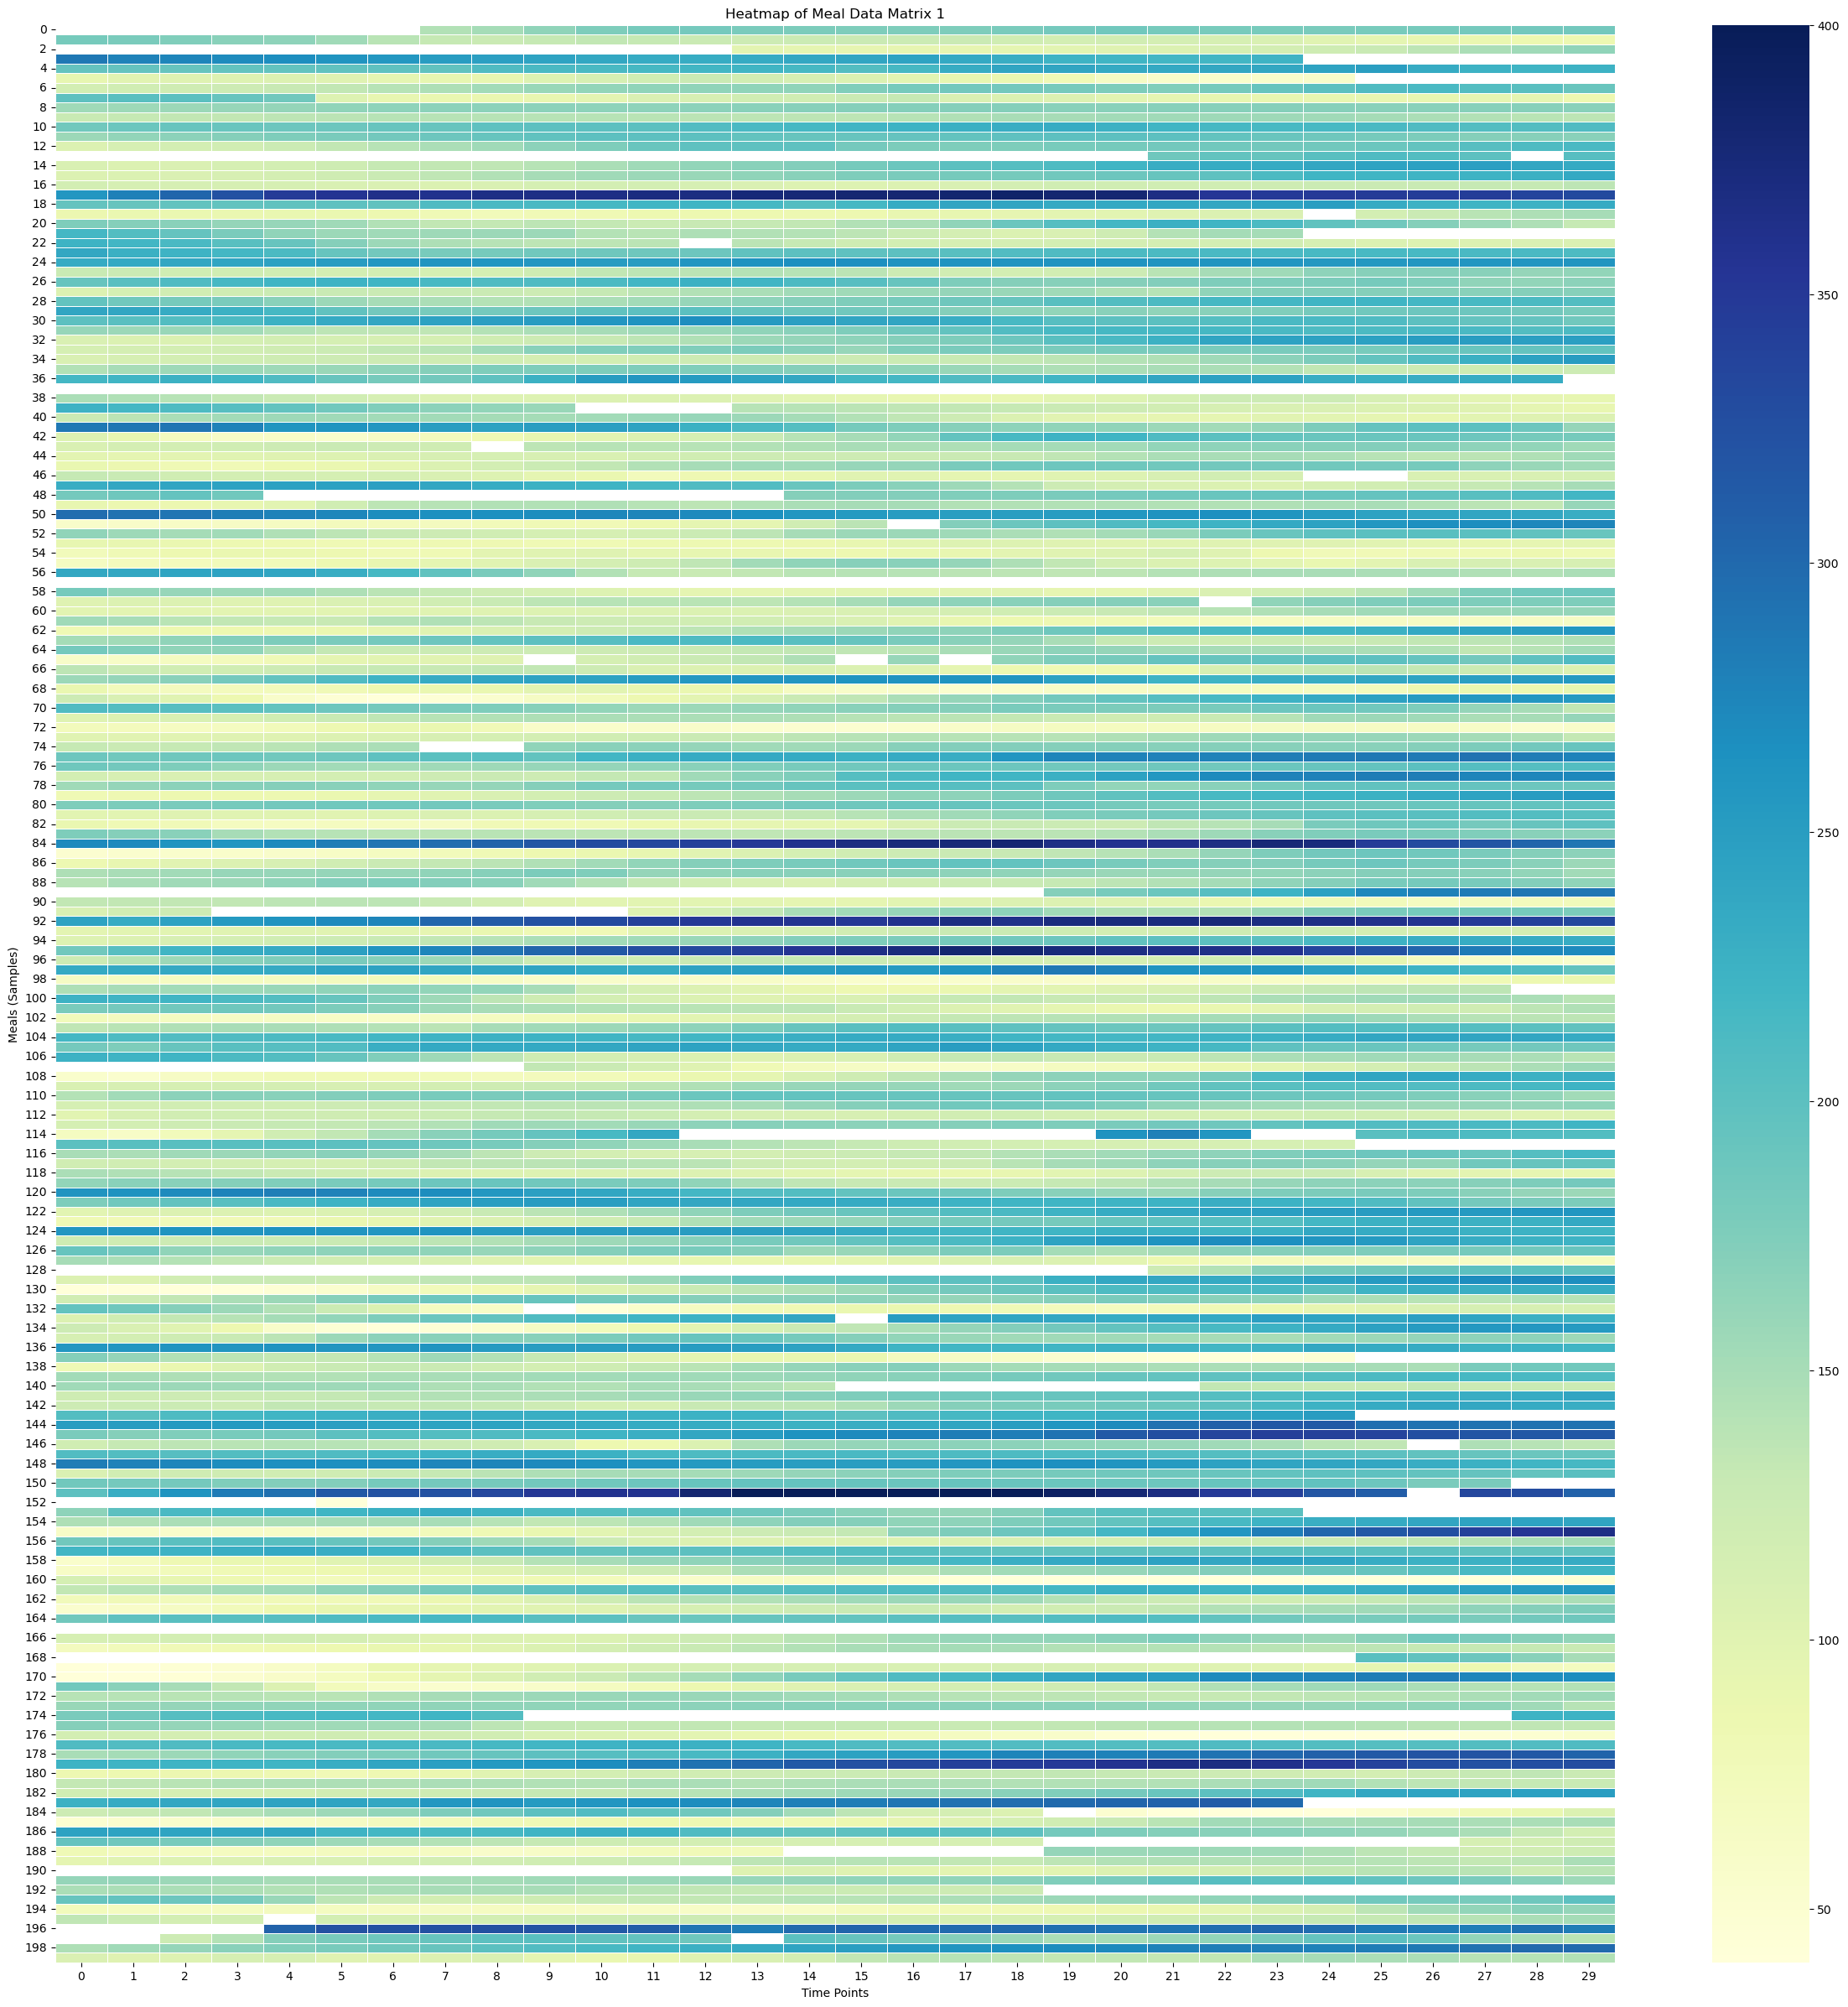
\includegraphics[width=0.7\linewidth]{files/a1f685b6fd0b25da1985e1bc18c26ec1.png}

\subparagraph{Surface Plot of Meal Data Matrix 1}

\begin{verbatim}
# Create X, Y meshgrid
X = np.arange(meal_data_matrix_1.shape[1])
Y = np.arange(meal_data_matrix_1.shape[0])
time_points = np.linspace( -30, 120, 30)  # X -axis: from -30 minutes to +120 minutes (30 time points)
meal_numbers = np.arange(1, len(meal_data_1) + 1)
X, Y = np.meshgrid(time_points, Y)
#X, Y = np.meshgrid(time_points, meal_numbers)
\end{verbatim}

\begin{verbatim}
X
\end{verbatim}

\begin{verbatim}
array([[ -30.        , -24.82758621, -19.65517241, ..., 109.65517241,
        114.82758621, 120.        ],
       [ -30.        , -24.82758621, -19.65517241, ..., 109.65517241,
        114.82758621, 120.        ],
       [ -30.        , -24.82758621, -19.65517241, ..., 109.65517241,
        114.82758621, 120.        ],
       ...,
       [ -30.        , -24.82758621, -19.65517241, ..., 109.65517241,
        114.82758621, 120.        ],
       [ -30.        , -24.82758621, -19.65517241, ..., 109.65517241,
        114.82758621, 120.        ],
       [ -30.        , -24.82758621, -19.65517241, ..., 109.65517241,
        114.82758621, 120.        ]])
\end{verbatim}

\begin{verbatim}
X.shape
\end{verbatim}

\begin{verbatim}
(715, 30)
\end{verbatim}

\begin{verbatim}
Y
\end{verbatim}

\begin{verbatim}
array([[  0,   0,   0, ...,   0,   0,   0],
       [  1,   1,   1, ...,   1,   1,   1],
       [  2,   2,   2, ...,   2,   2,   2],
       ...,
       [712, 712, 712, ..., 712, 712, 712],
       [713, 713, 713, ..., 713, 713, 713],
       [714, 714, 714, ..., 714, 714, 714]])
\end{verbatim}

\begin{verbatim}
# Fill NaNs using forward fill, then backward fill
meal_data_matrix_1_df = pd.DataFrame(meal_data_matrix_1)
meal_data_matrix_1_filled = meal_data_matrix_1_df.ffill().bfill().values
\end{verbatim}

\begin{verbatim}
# Apply a moving average smoothing to each row
window_size = 5  # Choose a window size for smoothing
smoothed_meal_data_matrix_1 = np.array([uniform_filter1d(row, size=window_size) for row in meal_data_matrix_1_filled])
\end{verbatim}

\begin{verbatim}
# Create the plot
fig = plt.figure(figsize=(10, 8))
ax = fig.add_subplot(111, projection='3d')
stride = 100

# Plot the surface
surface_plot = ax.plot_surface(X[::stride], Y[::stride], smoothed_meal_data_matrix_1[::stride], cmap='viridis', edgecolor='none')
ax.set_title('3D Surface Plot of Smoothed Averaged Meal Glucose Levels', y=0.985)
ax.set_xlabel('Time Relative to Start of Meal [minutes]', labelpad=10)
ax.set_ylabel('Meal Samples', labelpad=10)
#ax.set_zlabel('Glucose Level (mg/dL)', labelpad=30)

#ax.set_xticks(np.linspace( -30, 120, 7))

# Adjust axis limits to create a zoom -out effect
#ax.set_xlim( -30, 120)
ax.set_ylim(0, 800)
ax.set_zlim(0, 300)

fig.colorbar(surface_plot, ax=ax, shrink=0.5, aspect=10, label='Glucose Level (mg/dL)')

#plt.tight_layout()
fig.subplots_adjust(left=0.01, right=1, top=0.9, bottom=0.1)

ax.view_init(elev=25, azim= -55)

plt.show()
\end{verbatim}

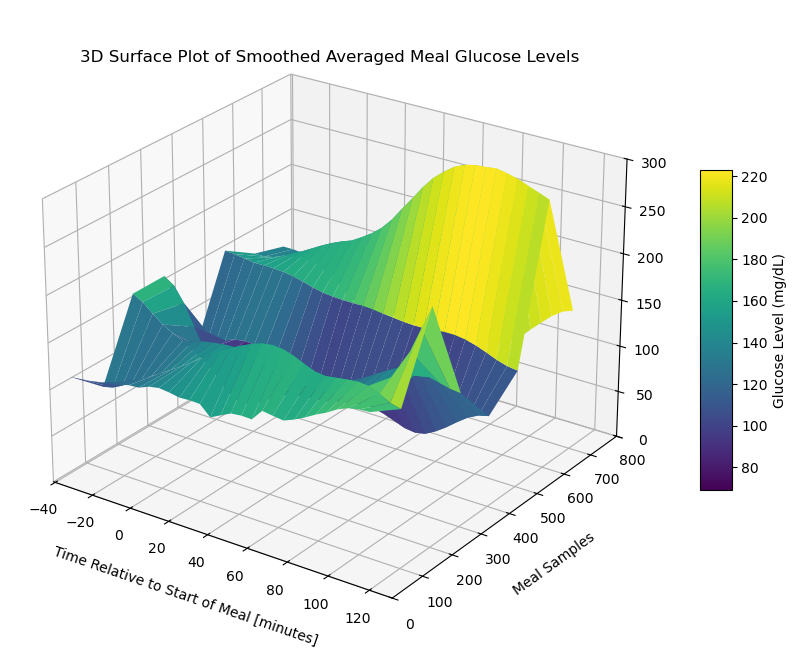
\includegraphics[width=0.7\linewidth]{files/a358ab8cc88548f7c8f091f310422644.png}

\subparagraph{Contour Plot of Meal Data Matrix 1}

\begin{verbatim}
# Create the contour plot
plt.figure(figsize=(15, 10))
plt.contourf(X, Y, meal_data_matrix_1_df, cmap='viridis', levels=30)
plt.colorbar(label='Glucose Level (mg/dL)')
plt.title('Contour Plot of Meal Glucose Levels')
plt.xlabel('Time Points')
plt.ylabel('Meal Samples')
plt.show()
\end{verbatim}

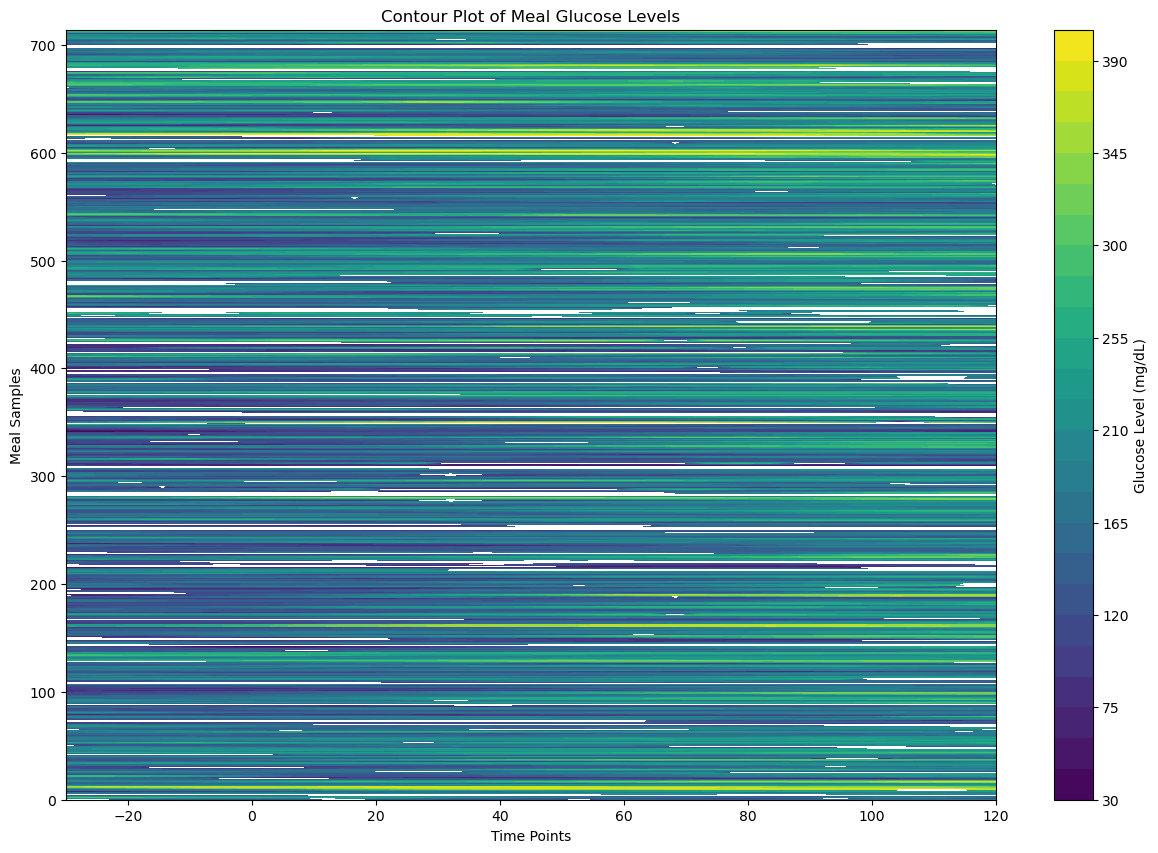
\includegraphics[width=0.7\linewidth]{files/126ddca12ae9dc0fcc519551eb88c0b8.png}

\subparagraph{Visualize Meal Data Matrix 2}

\subparagraph{Heatmap of Meal Data Matrix 2}

\begin{verbatim}
# Create the heatmap
sampled_meal_data_matrix_2 = meal_data_matrix_2[np.random.choice(meal_data_matrix_2.shape[0], 200, replace=False)]
plt.figure(figsize=(30, 30))
sns.heatmap(sampled_meal_data_matrix_2, cmap='YlGnBu', linewidths=0.5, annot=False, vmin=None, vmax=None)
plt.title('Heatmap of Meal Data Matrix 2')
plt.xlabel('Time Points')
plt.ylabel('Meals (Samples)')
plt.show()
\end{verbatim}

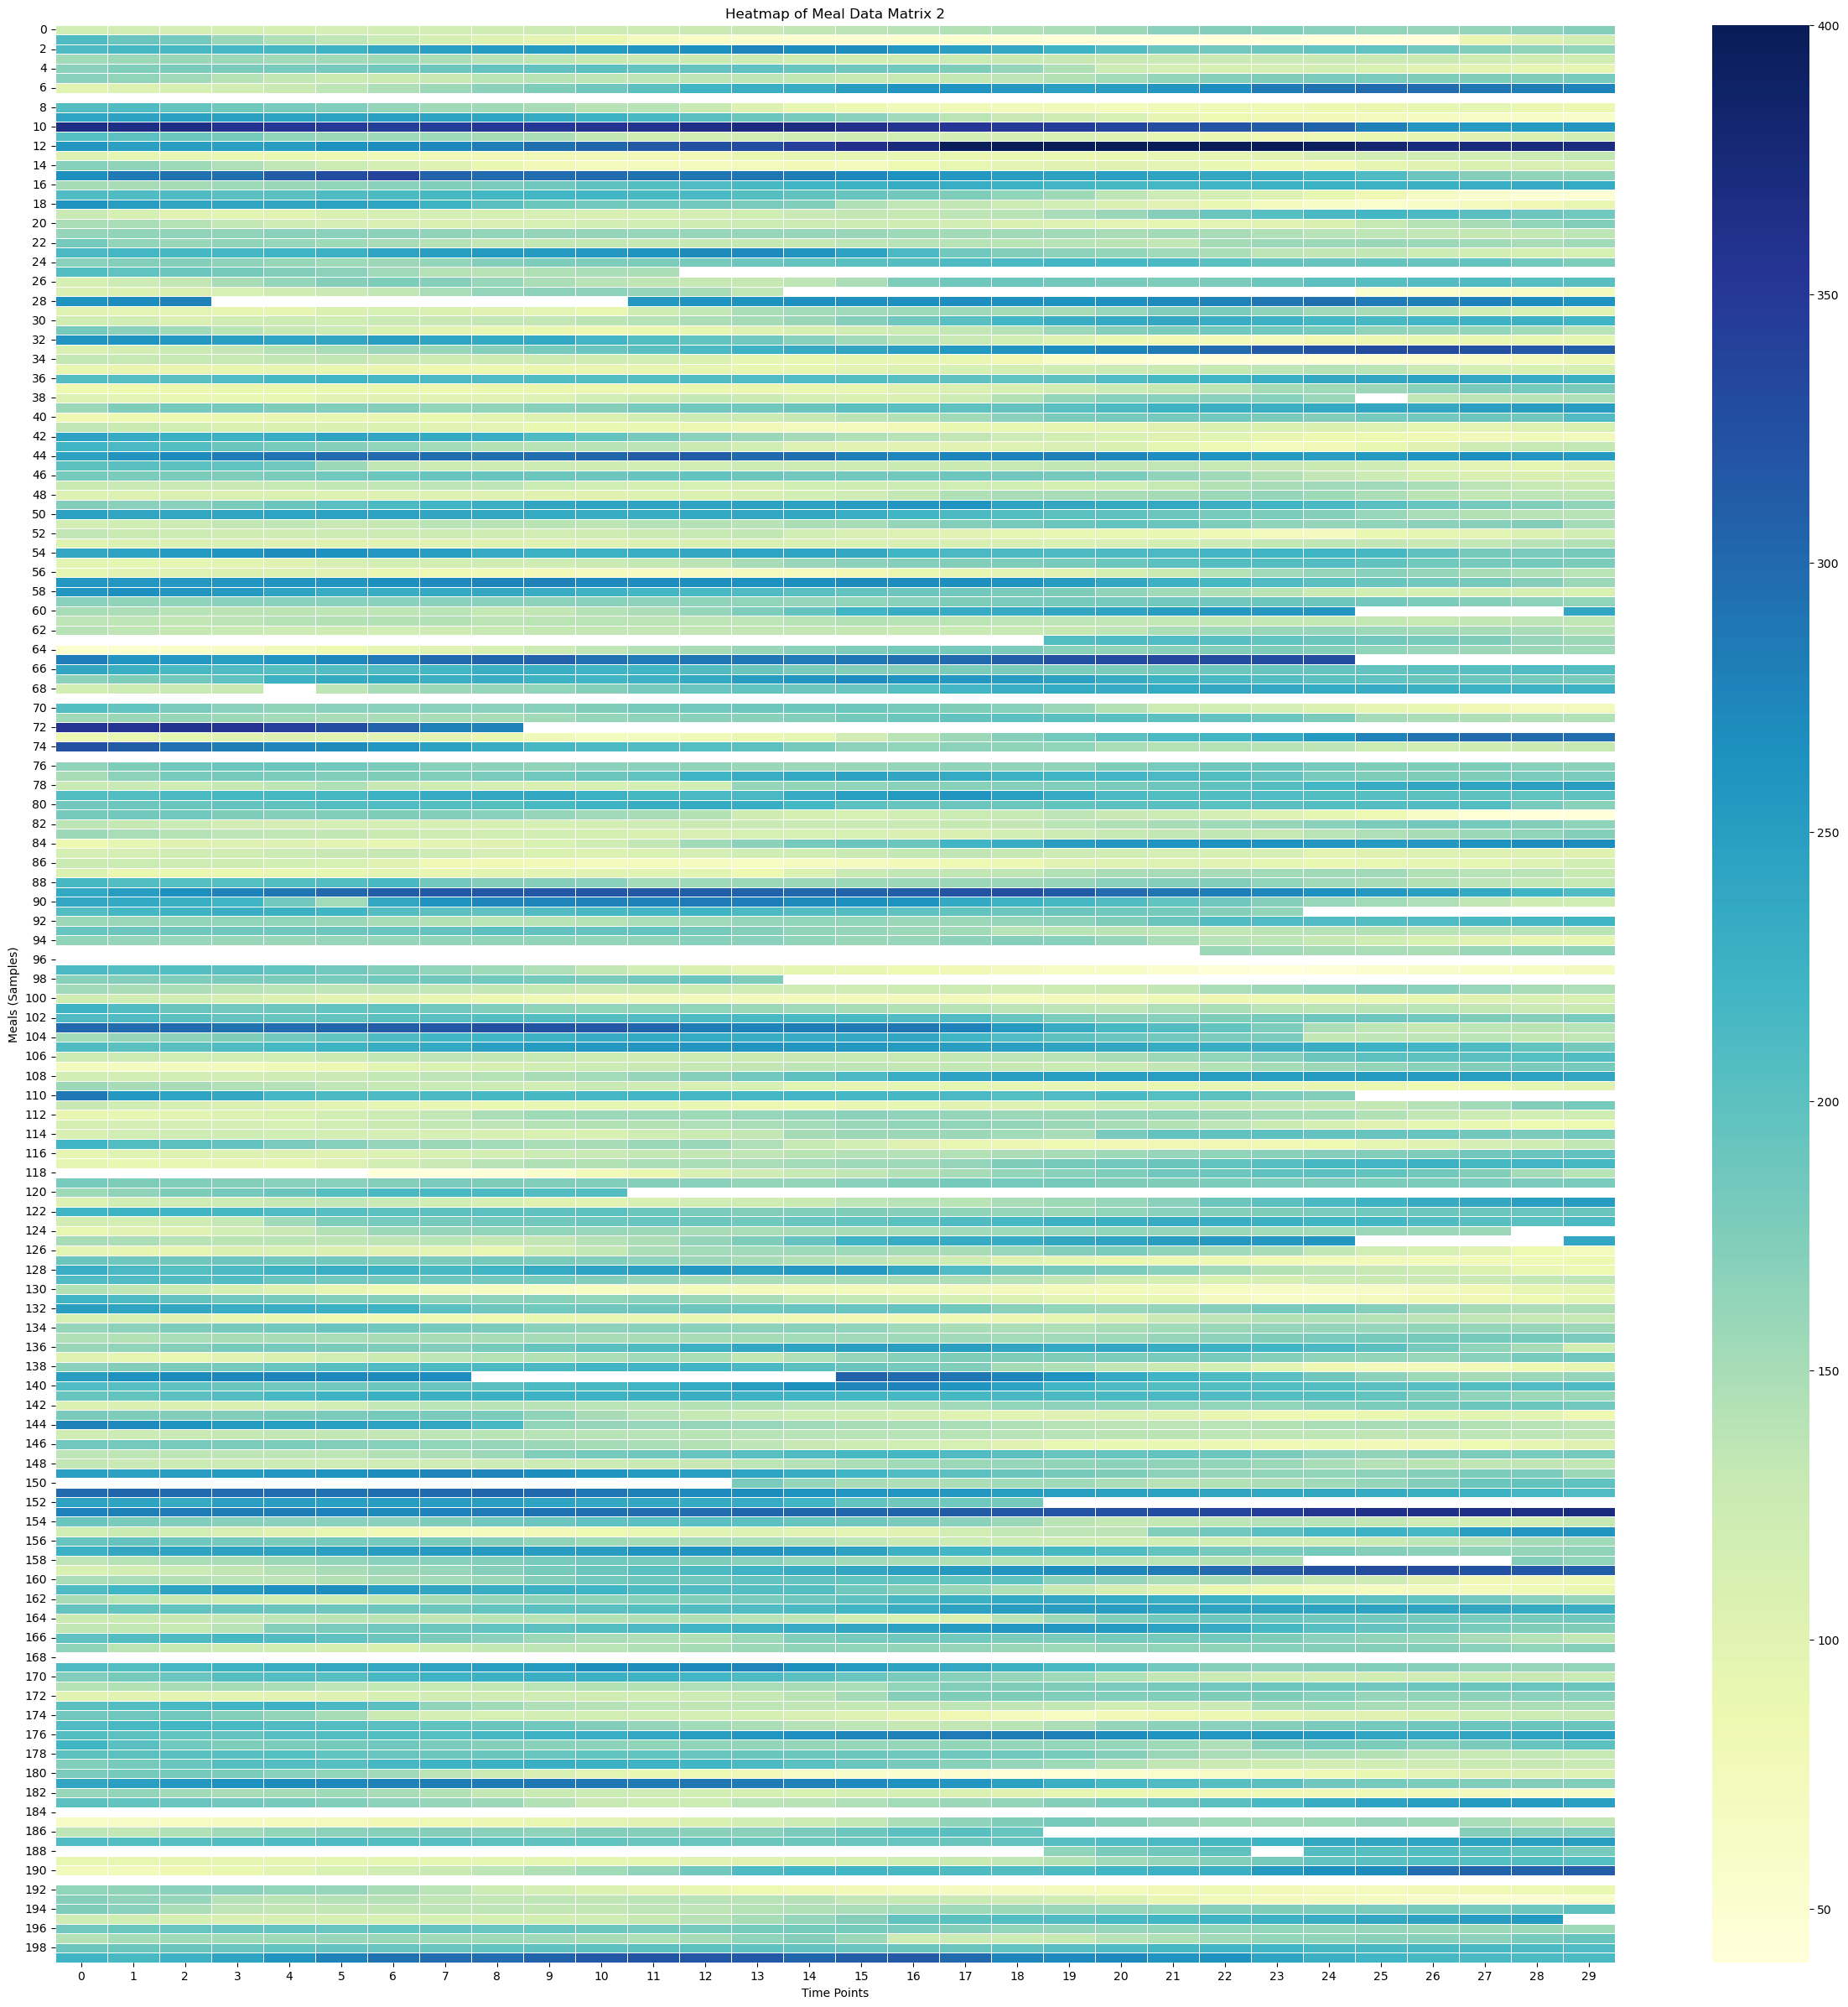
\includegraphics[width=0.7\linewidth]{files/82f82fc0c9bba17c87599c06cd8e4f27.png}

\subparagraph{Surface Plot of Meal Data Matrix 2}

\begin{verbatim}
# Create X, Y meshgrid
X = np.arange(meal_data_matrix_2.shape[1])
Y = np.arange(meal_data_matrix_2.shape[0])
time_points = np.linspace( -30, 120, 30)  # X -axis: from -30 minutes to +120 minutes (30 time points)
meal_numbers = np.arange(1, len(meal_data_2) + 1)
X, Y = np.meshgrid(time_points, Y)
#X, Y = np.meshgrid(time_points, meal_numbers)
\end{verbatim}

\begin{verbatim}
X
\end{verbatim}

\begin{verbatim}
array([[ -30.        , -24.82758621, -19.65517241, ..., 109.65517241,
        114.82758621, 120.        ],
       [ -30.        , -24.82758621, -19.65517241, ..., 109.65517241,
        114.82758621, 120.        ],
       [ -30.        , -24.82758621, -19.65517241, ..., 109.65517241,
        114.82758621, 120.        ],
       ...,
       [ -30.        , -24.82758621, -19.65517241, ..., 109.65517241,
        114.82758621, 120.        ],
       [ -30.        , -24.82758621, -19.65517241, ..., 109.65517241,
        114.82758621, 120.        ],
       [ -30.        , -24.82758621, -19.65517241, ..., 109.65517241,
        114.82758621, 120.        ]])
\end{verbatim}

\begin{verbatim}
X.shape
\end{verbatim}

\begin{verbatim}
(372, 30)
\end{verbatim}

\begin{verbatim}
Y
\end{verbatim}

\begin{verbatim}
array([[  0,   0,   0, ...,   0,   0,   0],
       [  1,   1,   1, ...,   1,   1,   1],
       [  2,   2,   2, ...,   2,   2,   2],
       ...,
       [369, 369, 369, ..., 369, 369, 369],
       [370, 370, 370, ..., 370, 370, 370],
       [371, 371, 371, ..., 371, 371, 371]])
\end{verbatim}

\begin{verbatim}
# Fill NaNs using forward fill, then backward fill
meal_data_matrix_2_df = pd.DataFrame(meal_data_matrix_2)
meal_data_matrix_2_filled = meal_data_matrix_2_df.ffill().bfill().values
\end{verbatim}

\begin{verbatim}
# Apply a moving average smoothing to each row
window_size = 5  # Choose a window size for smoothing
smoothed_meal_data_matrix_2 = np.array([uniform_filter1d(row, size=window_size) for row in meal_data_matrix_2_filled])
\end{verbatim}

\begin{verbatim}
# Create the plot
fig = plt.figure(figsize=(10, 8))
ax = fig.add_subplot(111, projection='3d')
stride = 100

# Plot the surface
surface_plot = ax.plot_surface(X[::stride], Y[::stride], smoothed_meal_data_matrix_2[::stride], cmap='viridis', edgecolor='none')
ax.set_title('3D Surface Plot of Smoothed Averaged Meal Glucose Levels', y=0.985)
ax.set_xlabel('Time Relative to Start of Meal [minutes]', labelpad=10)
ax.set_ylabel('Meal Samples', labelpad=10)
#ax.set_zlabel('Glucose Level (mg/dL)', labelpad=30)

#ax.set_xticks(np.linspace( -30, 120, 7))

# Adjust axis limits to create a zoom -out effect
#ax.set_xlim( -30, 120)
#ax.set_ylim(0, 800)
ax.set_zlim(0, 400)

fig.colorbar(surface_plot, ax=ax, shrink=0.5, aspect=10, label='Glucose Level (mg/dL)')

#plt.tight_layout()
fig.subplots_adjust(left=0.01, right=1, top=0.9, bottom=0.1)

ax.view_init(elev=25, azim= -55)

plt.show()
\end{verbatim}

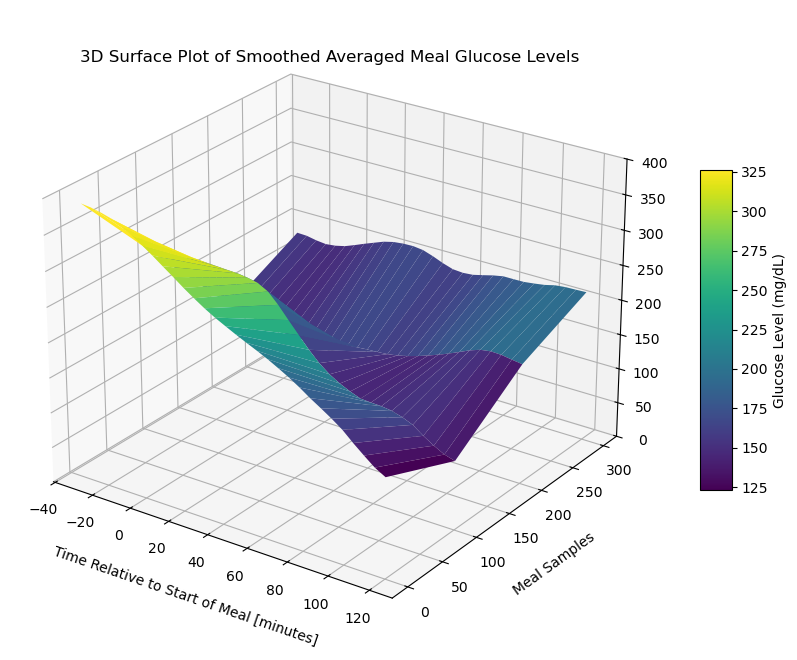
\includegraphics[width=0.7\linewidth]{files/70c826f5eb335eac4570cc114495306f.png}

\subparagraph{Contour Plot of Meal Data Matrix 2}

\begin{verbatim}
# Create the contour plot
plt.figure(figsize=(15, 10))
plt.contourf(X, Y, meal_data_matrix_2_df, cmap='viridis', levels=30)
plt.colorbar(label='Glucose Level (mg/dL)')
plt.title('Contour Plot of Meal Glucose Levels')
plt.xlabel('Time Points')
plt.ylabel('Meal Samples')
plt.show()
\end{verbatim}

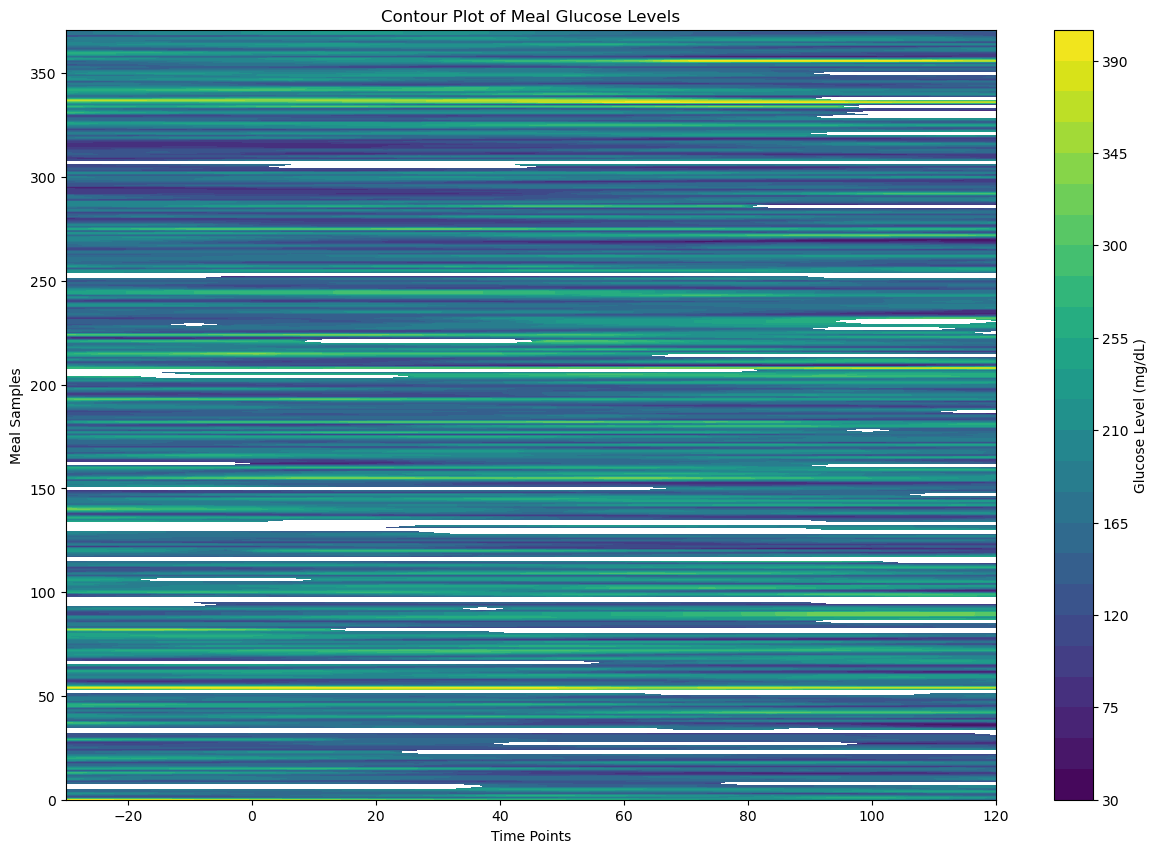
\includegraphics[width=0.7\linewidth]{files/23f4cbe824596a683b003752d28acd7d.png}

\subparagraph{Extract No - Meal Data}

\begin{verbatim}
# Initialize meal data list
no_meal_data_1 = []
    
# Loop through each meal start time to find valid post - absorbtive windows
for meal_time in meal_times_1:
    # Define the post -absorptive period: starts from tm+2 hours
    # and lasts 2 hours (i.e to four hours)
    post_absorptive_start = meal_time + pd.Timedelta(hours=2)
    post_absorptive_end = meal_time + pd.Timedelta(hours=4)
    
    # Check for meals in the post -absorptive period
    post_absorptive_meals = insulin_data_1[(insulin_data_1['datetime'] >= post_absorptive_start) &
                                         (insulin_data_1['datetime'] <= post_absorptive_end)]
    
    # Step 2 Condition (a): If any non -zero, non -NaN meal is found in the
    # post -absorptive period, skip this stretch
    if not post_absorptive_meals.empty:
        # Check if any of the meals have a non -zero carb input
        if (post_absorptive_meals['BWZ Carb Input (grams)'] > 0).any():
            # Skip this stretch, as there is a meal found in the post -absorptive period
            continue
    
    # Step 2 condition (b): If meal values are 0 or NaN, ignore and consider the stretch
    # Extract the corresponding 2 -hour CGM data
    no_meal_cgm_data_1 = cgm_data_1[(cgm_data_1['datetime'] >= post_absorptive_start) & 
                                (cgm_data_1['datetime'] <= post_absorptive_end)]
    
    # Check if the extracted data has the correct number of points (24 for no meal data)
    if len(no_meal_cgm_data_1) == 24:
        no_meal_data_1.append(no_meal_cgm_data_1['Sensor Glucose (mg/dL)'].values)
\end{verbatim}

\begin{verbatim}
# Initialize meal data list
no_meal_data_2 = []
    
# Loop through each meal start time to find valid post - absorbtive windows
for meal_time in meal_times_2:
    # Define the post -absorptive period: starts from tm+2 hours
    # and lasts 2 hours (i.e to four hours)
    post_absorptive_start = meal_time + pd.Timedelta(hours=2)
    post_absorptive_end = meal_time + pd.Timedelta(hours=4)
    
    # Check for meals in the post -absorptive period
    post_absorptive_meals = insulin_data_2[(insulin_data_2['datetime'] >= post_absorptive_start) &
                                         (insulin_data_2['datetime'] <= post_absorptive_end)]
    
    # Step 2 Condition (a): If any non -zero, non -NaN meal is found in the
    # post -absorptive period, skip this stretch
    if not post_absorptive_meals.empty:
        # Check if any of the meals have a non -zero carb input
        if (post_absorptive_meals['BWZ Carb Input (grams)'] > 0).any():
            # Skip this stretch, as there is a meal found in the post -absorptive period
            continue
    
    # Step 2 condition (b): If meal values are 0 or NaN, ignore and consider the stretch
    # Extract the corresponding 2 -hour CGM data
    no_meal_cgm_data_2 = cgm_data_2[(cgm_data_2['datetime'] >= post_absorptive_start) & 
                                (cgm_data_2['datetime'] <= post_absorptive_end)]
    
    # Check if the extracted data has the correct number of points (24 for no meal data)
    if len(no_meal_cgm_data_2) == 24:
        no_meal_data_2.append(no_meal_cgm_data_2['Sensor Glucose (mg/dL)'].values)
\end{verbatim}

\begin{verbatim}
len(no_meal_data_1)
\end{verbatim}

\begin{verbatim}
510
\end{verbatim}

\begin{verbatim}
len(no_meal_data_2)
\end{verbatim}

\begin{verbatim}
325
\end{verbatim}

\begin{verbatim}
#no_meal_data_1[0:5]
\end{verbatim}

\begin{verbatim}
#no_meal_data_2[0:5]
\end{verbatim}

\subparagraph{Create No Meal Data Matrix}

\begin{verbatim}
no_meal_data_matrix_1 = np.array(no_meal_data_1)
#no_meal_data_matrix_1
\end{verbatim}

\begin{verbatim}
no_meal_data_matrix_2 = np.array(no_meal_data_2)
#no_meal_data_matrix_2
\end{verbatim}

\begin{verbatim}
no_meal_data_matrix_1.shape
\end{verbatim}

\begin{verbatim}
(510, 24)
\end{verbatim}

\begin{verbatim}
no_meal_data_matrix_2.shape
\end{verbatim}

\begin{verbatim}
(325, 24)
\end{verbatim}

\subparagraph{Visualize No Meal Data Matrix 1}

\subparagraph{Heatmap of No Meal Data Matrix 1}

\begin{verbatim}
# Create the heatmap
sampled_no_meal_data_matrix_1 = no_meal_data_matrix_1[np.random.choice(no_meal_data_matrix_1.shape[0], 200, replace=False)]
plt.figure(figsize=(30, 30))
sns.heatmap(sampled_no_meal_data_matrix_1, cmap='YlGnBu', linewidths=0.5, annot=False, vmin=None, vmax=None)
plt.title('Heatmap of No Meal Data Matrix 1')
plt.xlabel('Time Points')
plt.ylabel('Meals (Samples)')
plt.show()
\end{verbatim}

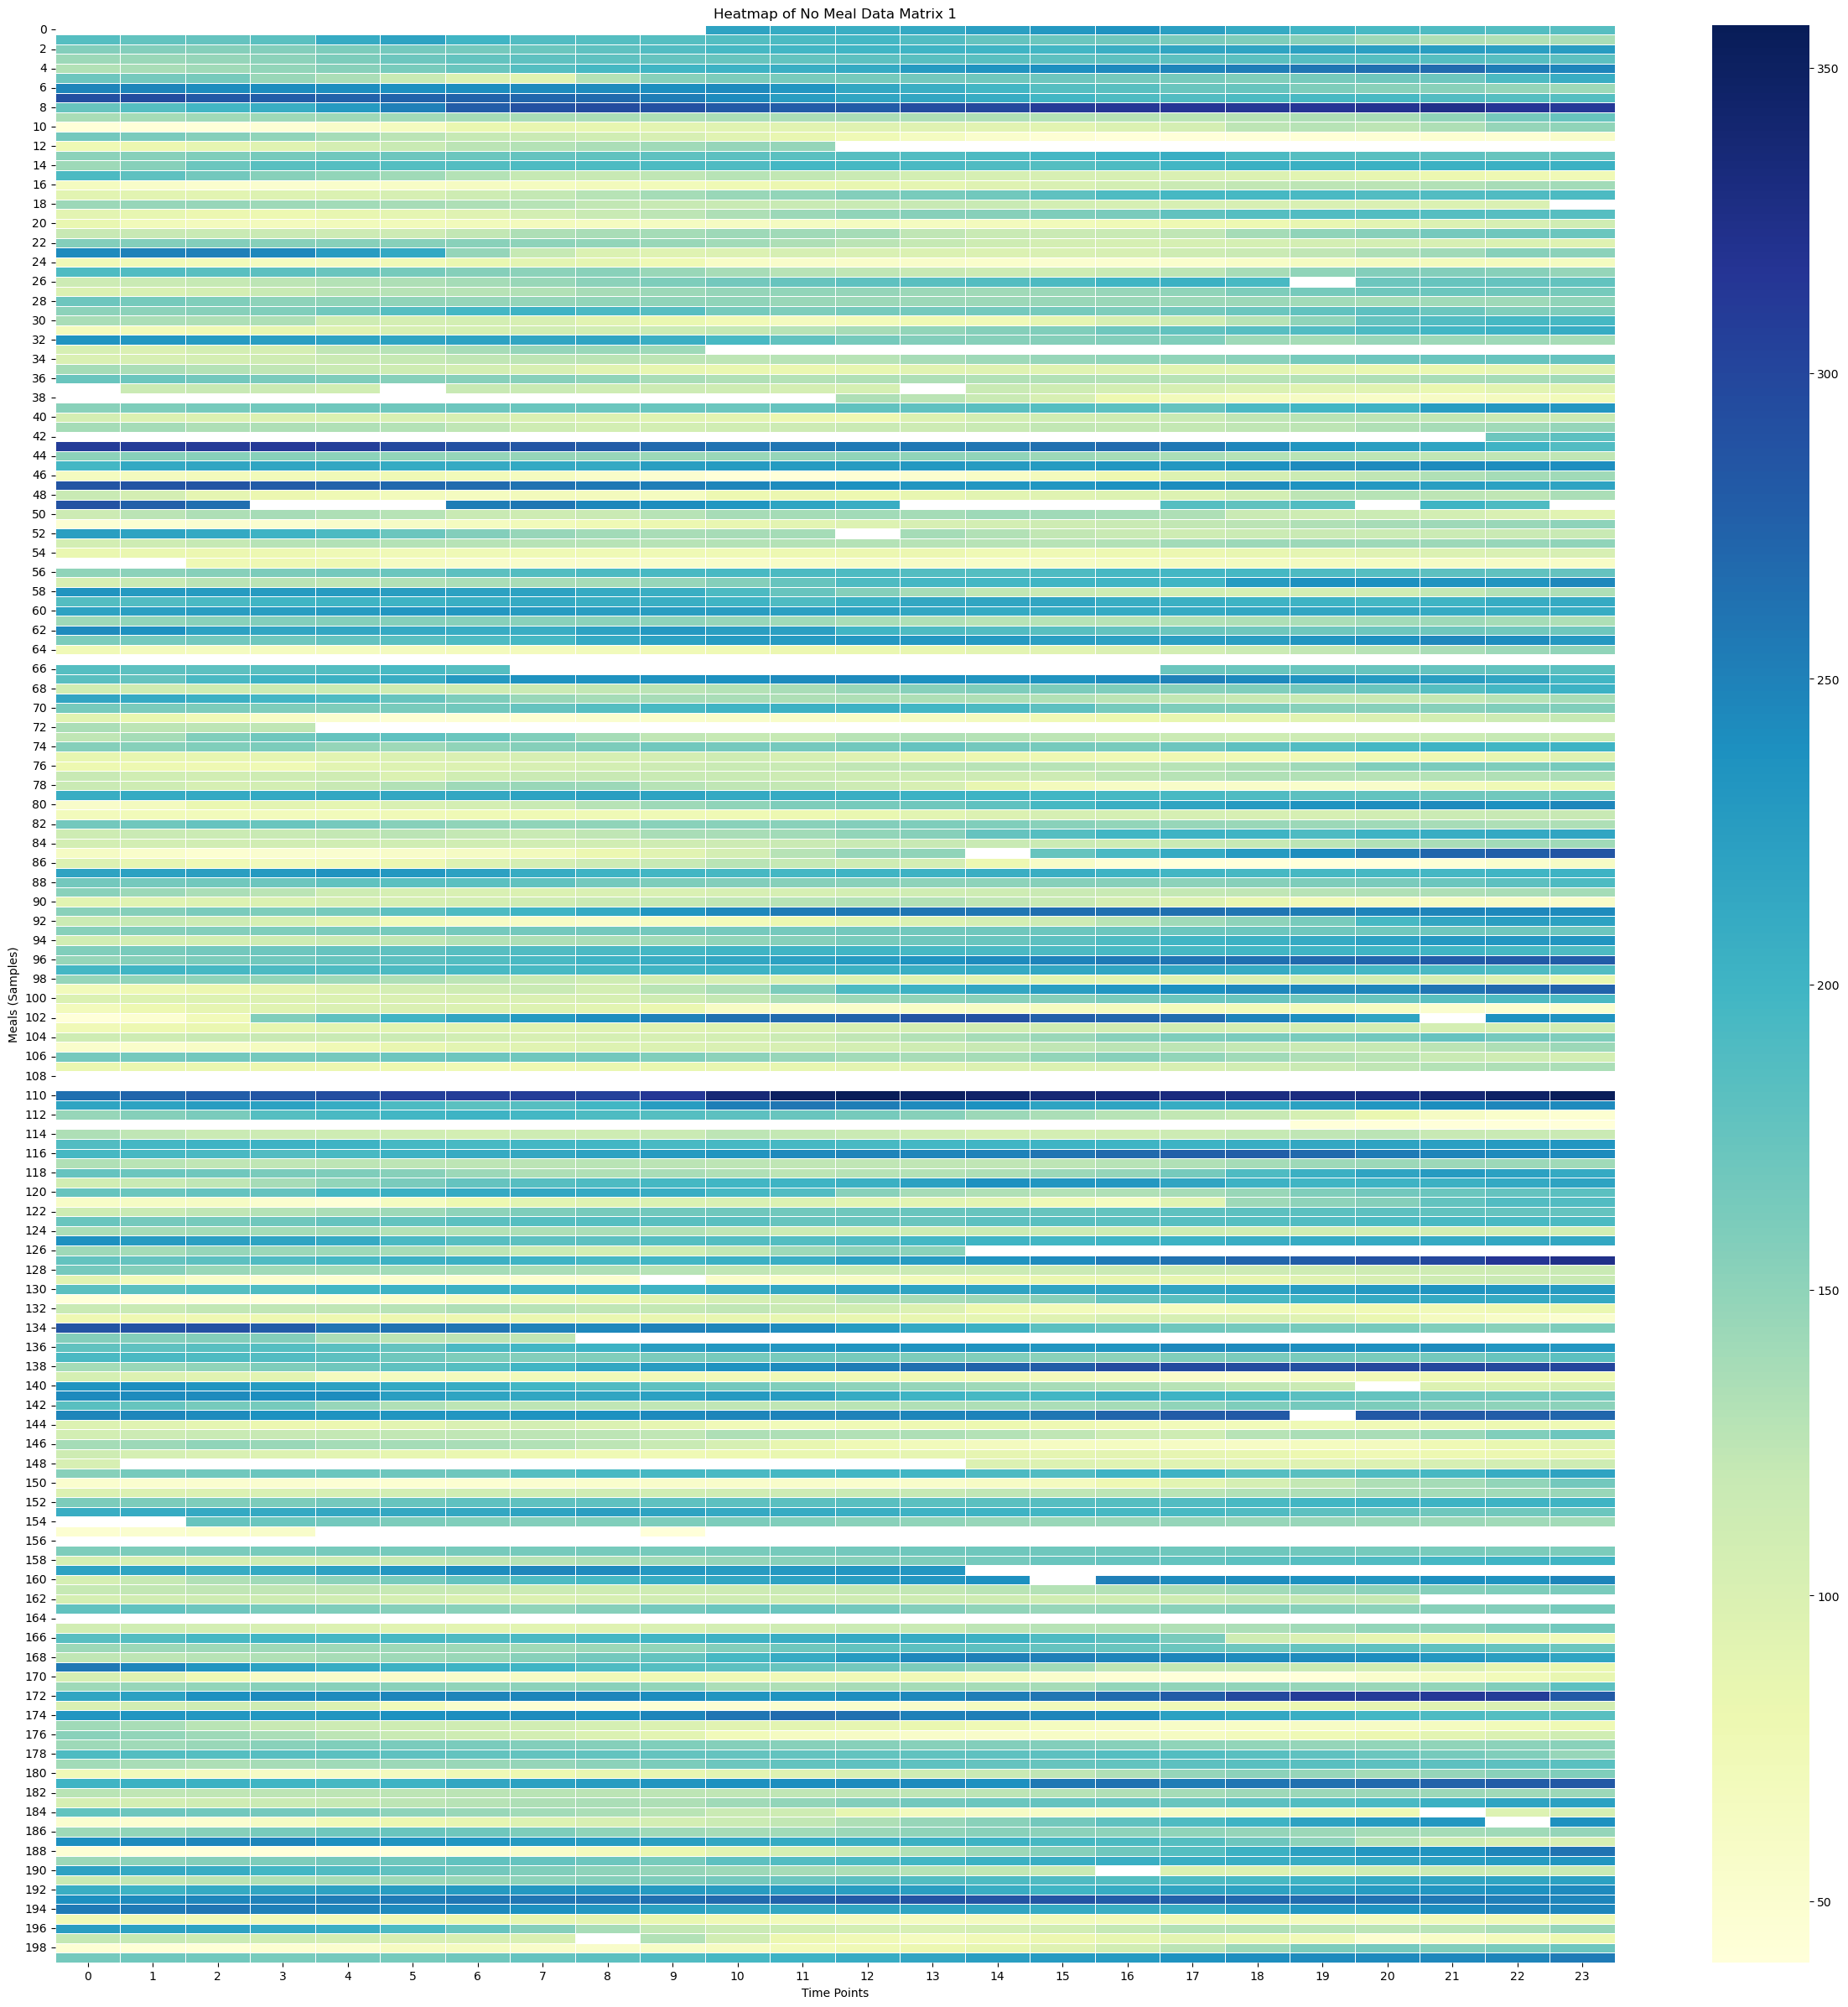
\includegraphics[width=0.7\linewidth]{files/b0cde087ebdd9a43dde2e268f39de683.png}

\subparagraph{Surface Plot of No Meal Data Matrix 1}

\begin{verbatim}
time_points = np.linspace( -30, 120, 24)
print(time_points)
print(time_points.shape)
\end{verbatim}

\begin{verbatim}
[ -30.         -23.47826087 -16.95652174 -10.43478261  -3.91304348
   2.60869565   9.13043478  15.65217391  22.17391304  28.69565217
  35.2173913   41.73913043  48.26086957  54.7826087   61.30434783
  67.82608696  74.34782609  80.86956522  87.39130435  93.91304348
 100.43478261 106.95652174 113.47826087 120.        ]
(24,)
\end{verbatim}

\begin{verbatim}
# Create X, Y meshgrid
X = np.arange(no_meal_data_matrix_1.shape[1])
Y = np.arange(no_meal_data_matrix_1.shape[0])
time_points = np.linspace( -30, 120, 24)  # X -axis: from -30 minutes to +120 minutes (24 time points)
meal_numbers = np.arange(1, len(no_meal_data_1) + 1)
X, Y = np.meshgrid(time_points, Y)
#X, Y = np.meshgrid(time_points, meal_numbers)
\end{verbatim}

\begin{verbatim}
X
\end{verbatim}

\begin{verbatim}
array([[ -30.        , -23.47826087, -16.95652174, ..., 106.95652174,
        113.47826087, 120.        ],
       [ -30.        , -23.47826087, -16.95652174, ..., 106.95652174,
        113.47826087, 120.        ],
       [ -30.        , -23.47826087, -16.95652174, ..., 106.95652174,
        113.47826087, 120.        ],
       ...,
       [ -30.        , -23.47826087, -16.95652174, ..., 106.95652174,
        113.47826087, 120.        ],
       [ -30.        , -23.47826087, -16.95652174, ..., 106.95652174,
        113.47826087, 120.        ],
       [ -30.        , -23.47826087, -16.95652174, ..., 106.95652174,
        113.47826087, 120.        ]])
\end{verbatim}

\begin{verbatim}
X.shape
\end{verbatim}

\begin{verbatim}
(510, 24)
\end{verbatim}

\begin{verbatim}
Y
\end{verbatim}

\begin{verbatim}
array([[  0,   0,   0, ...,   0,   0,   0],
       [  1,   1,   1, ...,   1,   1,   1],
       [  2,   2,   2, ...,   2,   2,   2],
       ...,
       [507, 507, 507, ..., 507, 507, 507],
       [508, 508, 508, ..., 508, 508, 508],
       [509, 509, 509, ..., 509, 509, 509]])
\end{verbatim}

\begin{verbatim}
Y.shape
\end{verbatim}

\begin{verbatim}
(510, 24)
\end{verbatim}

\begin{verbatim}
# Fill NaNs using forward fill, then backward fill
no_meal_data_matrix_1_df = pd.DataFrame(no_meal_data_matrix_1)
no_meal_data_matrix_1_filled = no_meal_data_matrix_1_df.ffill().bfill().values
\end{verbatim}

\begin{verbatim}
# Apply a moving average smoothing to each row
window_size = 5  # Choose a window size for smoothing
smoothed_no_meal_data_matrix_1 = np.array([uniform_filter1d(row, size=window_size) for row in no_meal_data_matrix_1_filled])
\end{verbatim}

\begin{verbatim}
# Create the plot
fig = plt.figure(figsize=(10, 8))
ax = fig.add_subplot(111, projection='3d')
stride = 100

# Plot the surface
surface_plot = ax.plot_surface(X[::stride], Y[::stride], smoothed_no_meal_data_matrix_1[::stride], cmap='viridis', edgecolor='none')
ax.set_title('3D Surface Plot of Smoothed Averaged No Meal Glucose Levels', y=0.985)
ax.set_xlabel('Time Relative to End of Meal [minutes]', labelpad=10)
ax.set_ylabel('Meal Samples', labelpad=10)
#ax.set_zlabel('Glucose Level (mg/dL)', labelpad=30)

#ax.set_xticks(np.linspace( -30, 120, 7))

# Adjust axis limits to create a zoom -out effect
#ax.set_xlim( -30, 120)
#ax.set_ylim(0, 800)
#ax.set_zlim(0, 300)

fig.colorbar(surface_plot, ax=ax, shrink=0.5, aspect=10, label='Glucose Level (mg/dL)')

#plt.tight_layout()
fig.subplots_adjust(left=0.01, right=1, top=0.9, bottom=0.1)

ax.view_init(elev=25, azim= -55)

plt.show()
\end{verbatim}

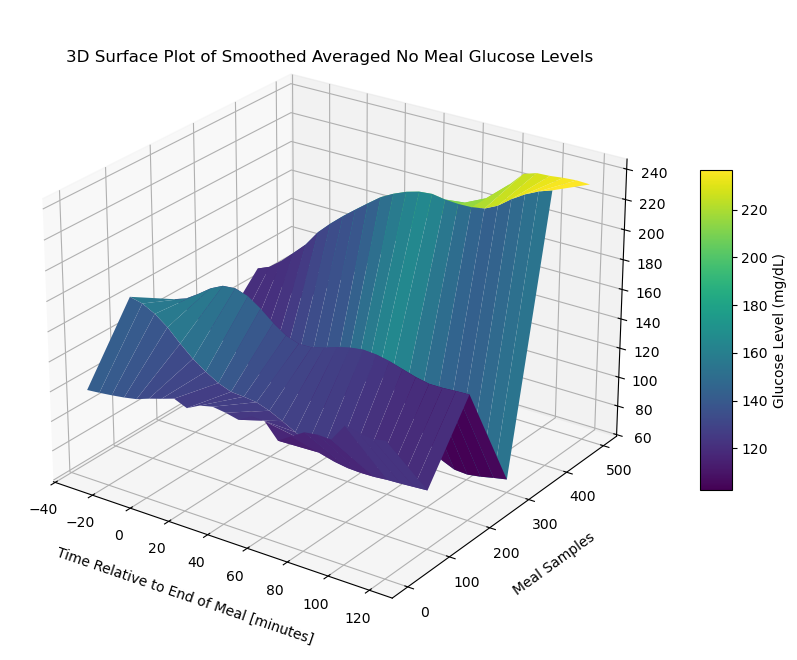
\includegraphics[width=0.7\linewidth]{files/852e2b3b38614cf71d1db9b868b4224f.png}

\subparagraph{Contour Plot of No Meal Data Matrix 1}

\begin{verbatim}
# Create the contour plot
plt.figure(figsize=(15, 10))
plt.contourf(X, Y, no_meal_data_matrix_1_df, cmap='viridis', levels=30)
plt.colorbar(label='Glucose Level (mg/dL)')
plt.title('Contour Plot of No Meal Glucose Levels')
plt.xlabel('Time Points')
plt.ylabel('Meal Samples')
plt.show()
\end{verbatim}

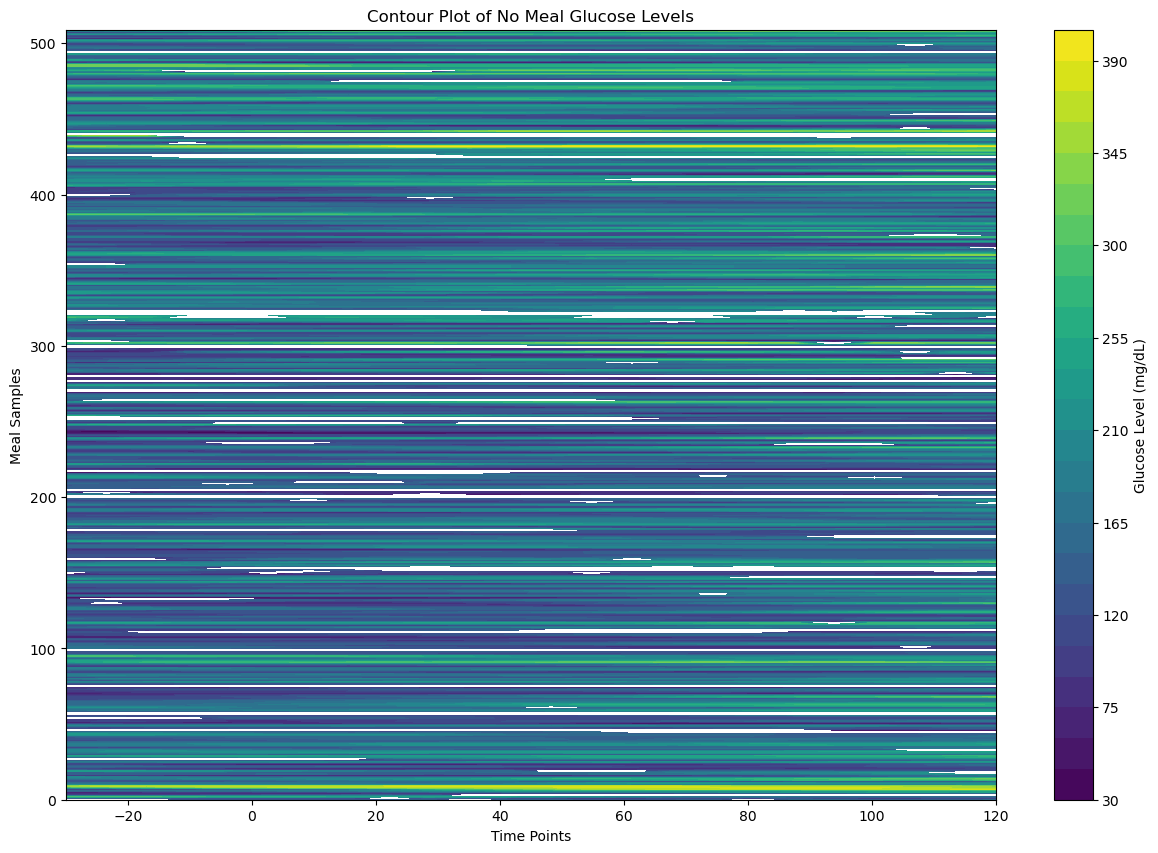
\includegraphics[width=0.7\linewidth]{files/fd34e6f01e7c7e3e118f37add522c9b2.png}

\subparagraph{Visualize No Meal Data Matrix 2}

\subparagraph{Heatmap of No Meal Data Matrix 2}

\begin{verbatim}
# Create the heatmap
sampled_no_meal_data_matrix_2 = no_meal_data_matrix_2[np.random.choice(no_meal_data_matrix_2.shape[0], 200, replace=False)]
plt.figure(figsize=(30, 30))
sns.heatmap(sampled_meal_data_matrix_2, cmap='YlGnBu', linewidths=0.5, annot=False, vmin=None, vmax=None)
plt.title('Heatmap of No Meal Data Matrix 1')
plt.xlabel('Time Points')
plt.ylabel('Meals (Samples)')
plt.show()
\end{verbatim}

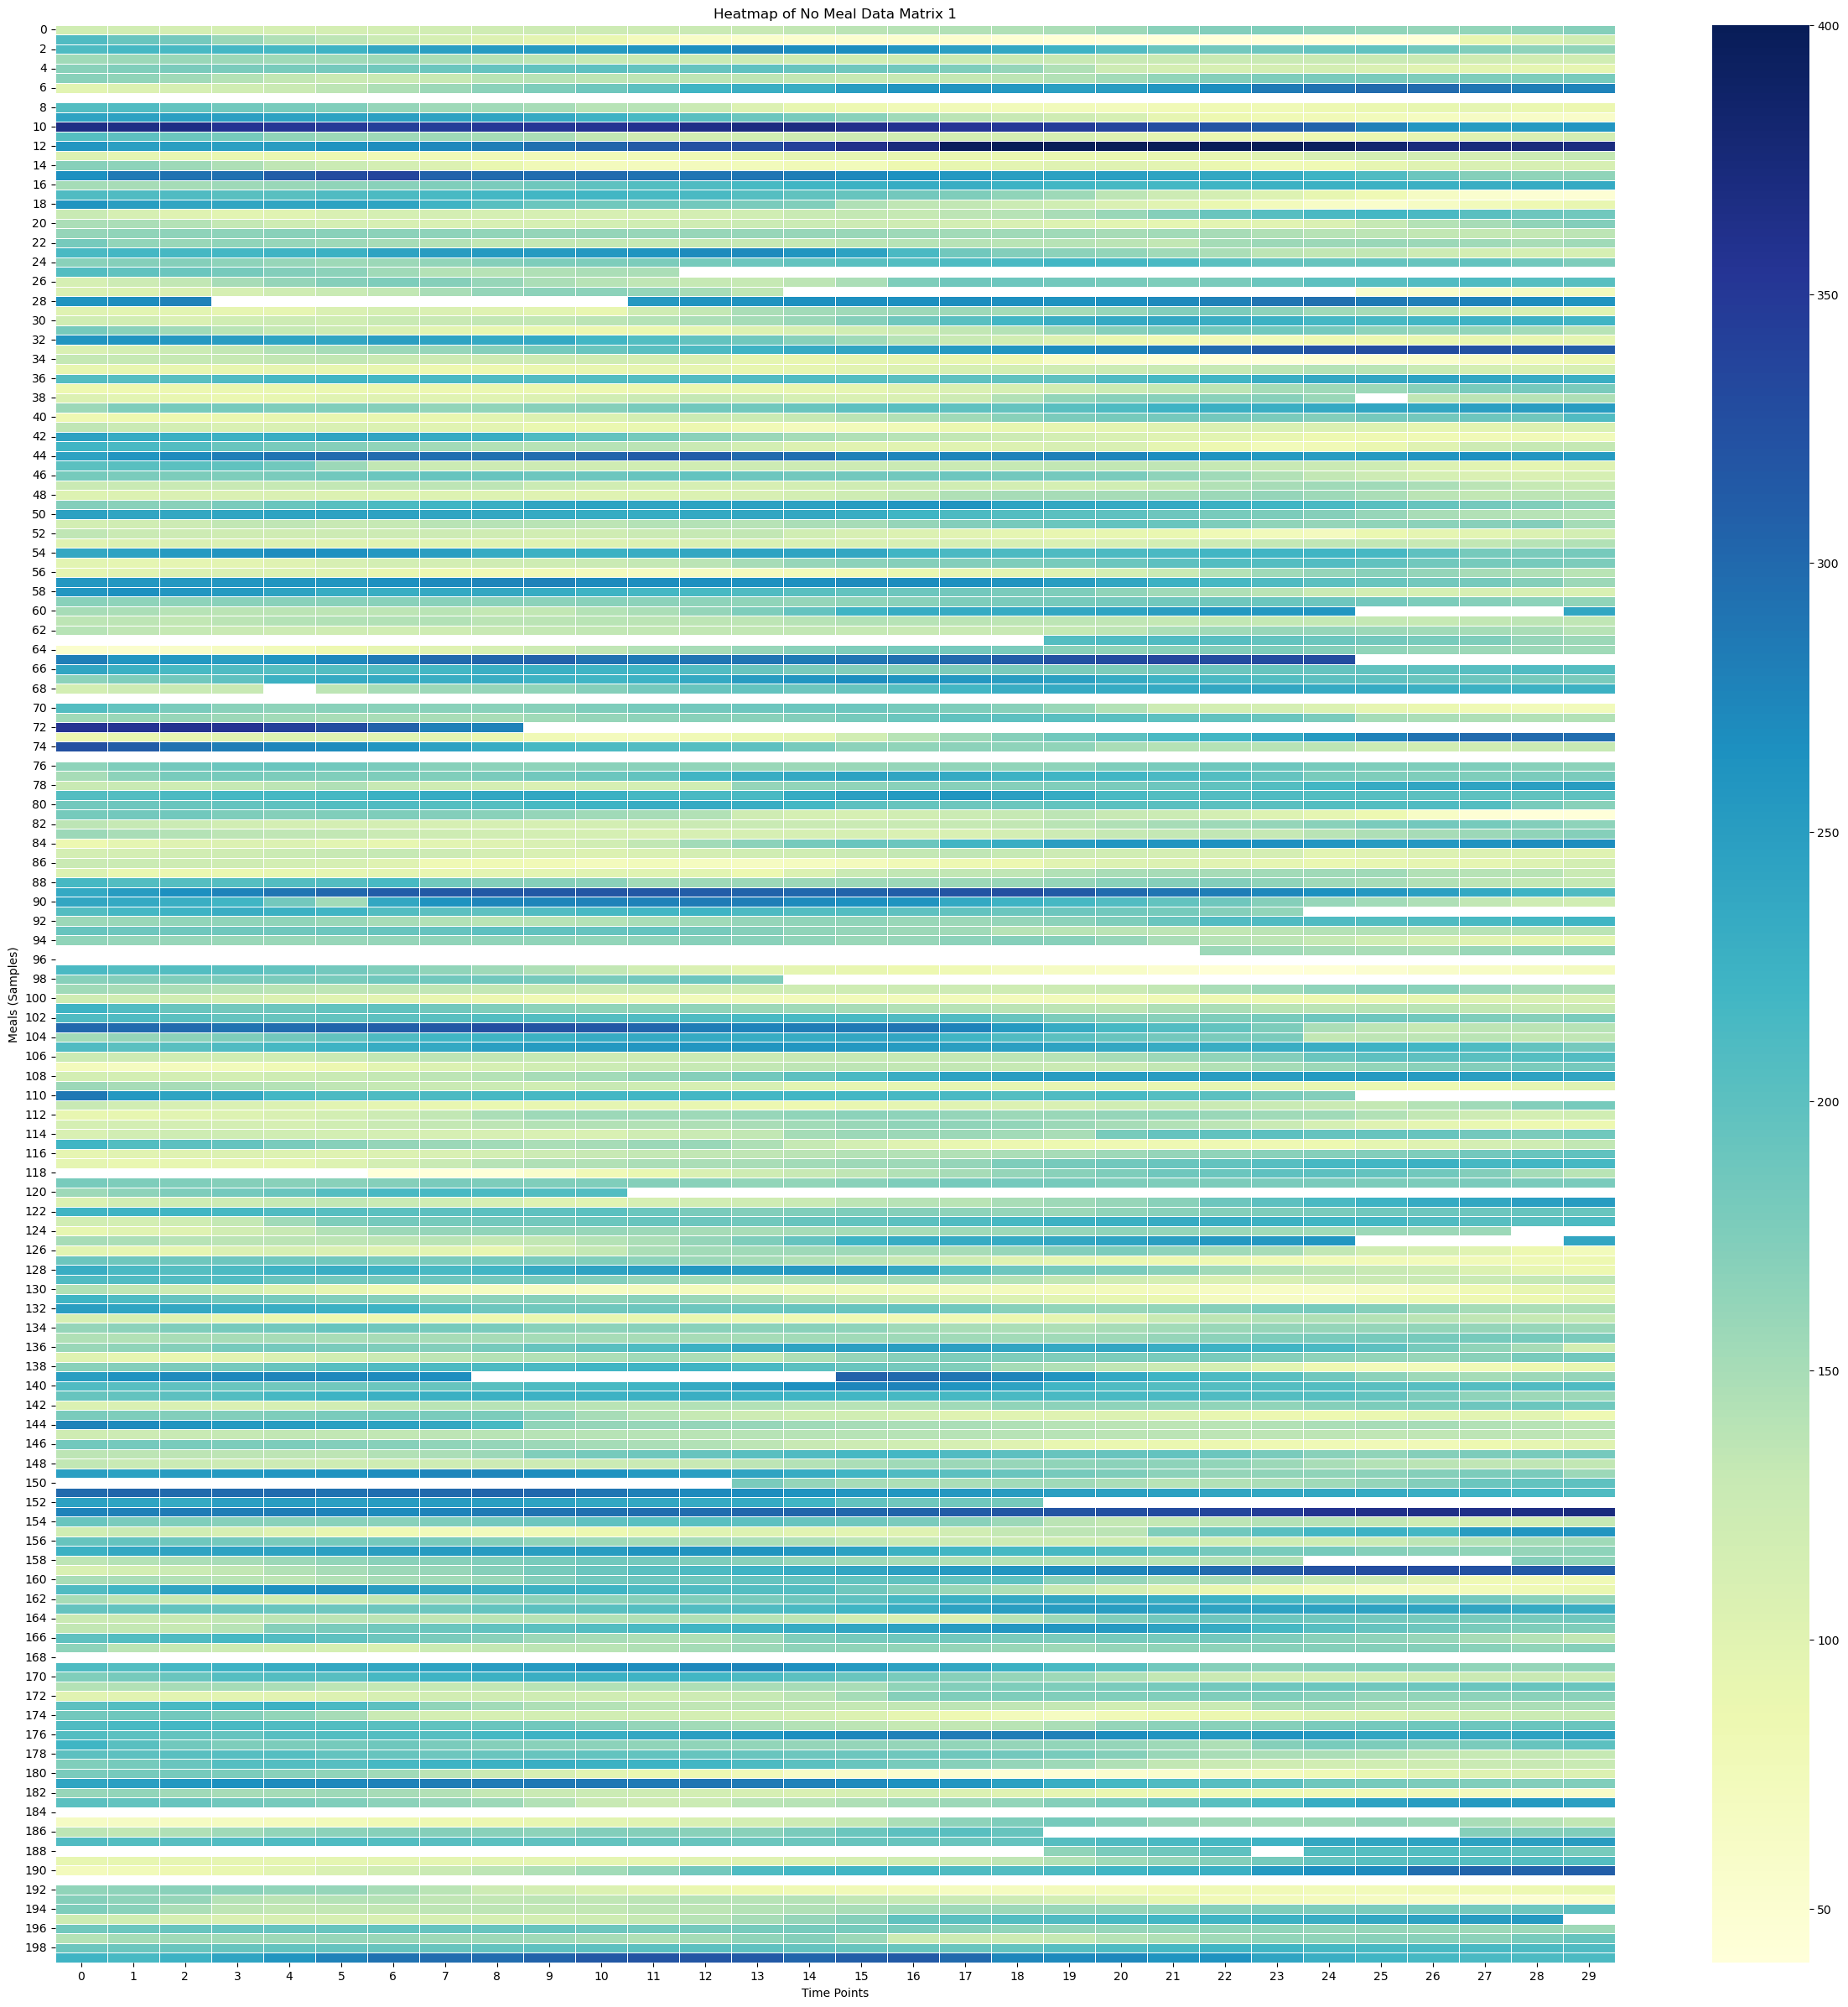
\includegraphics[width=0.7\linewidth]{files/38dbc59a10c3bb9ea4ce45782e7631d0.png}

\subparagraph{Surface Plot of No Meal Data Matrix 2}

\begin{verbatim}
time_points = np.linspace( -30, 120, 24)
print(time_points)
print(time_points.shape)
\end{verbatim}

\begin{verbatim}
[ -30.         -23.47826087 -16.95652174 -10.43478261  -3.91304348
   2.60869565   9.13043478  15.65217391  22.17391304  28.69565217
  35.2173913   41.73913043  48.26086957  54.7826087   61.30434783
  67.82608696  74.34782609  80.86956522  87.39130435  93.91304348
 100.43478261 106.95652174 113.47826087 120.        ]
(24,)
\end{verbatim}

\begin{verbatim}
# Create X, Y meshgrid
X = np.arange(no_meal_data_matrix_2.shape[1])
Y = np.arange(no_meal_data_matrix_2.shape[0])
time_points = np.linspace( -30, 120, 24)  # X -axis: from -30 minutes to +120 minutes (24 time points)
meal_numbers = np.arange(1, len(no_meal_data_2) + 1)
X, Y = np.meshgrid(time_points, Y)
#X, Y = np.meshgrid(time_points, meal_numbers)
\end{verbatim}

\begin{verbatim}
X
\end{verbatim}

\begin{verbatim}
array([[ -30.        , -23.47826087, -16.95652174, ..., 106.95652174,
        113.47826087, 120.        ],
       [ -30.        , -23.47826087, -16.95652174, ..., 106.95652174,
        113.47826087, 120.        ],
       [ -30.        , -23.47826087, -16.95652174, ..., 106.95652174,
        113.47826087, 120.        ],
       ...,
       [ -30.        , -23.47826087, -16.95652174, ..., 106.95652174,
        113.47826087, 120.        ],
       [ -30.        , -23.47826087, -16.95652174, ..., 106.95652174,
        113.47826087, 120.        ],
       [ -30.        , -23.47826087, -16.95652174, ..., 106.95652174,
        113.47826087, 120.        ]])
\end{verbatim}

\begin{verbatim}
X.shape
\end{verbatim}

\begin{verbatim}
(325, 24)
\end{verbatim}

\begin{verbatim}
Y
\end{verbatim}

\begin{verbatim}
array([[  0,   0,   0, ...,   0,   0,   0],
       [  1,   1,   1, ...,   1,   1,   1],
       [  2,   2,   2, ...,   2,   2,   2],
       ...,
       [322, 322, 322, ..., 322, 322, 322],
       [323, 323, 323, ..., 323, 323, 323],
       [324, 324, 324, ..., 324, 324, 324]])
\end{verbatim}

\begin{verbatim}
Y.shape
\end{verbatim}

\begin{verbatim}
(325, 24)
\end{verbatim}

\begin{verbatim}
# Fill NaNs using forward fill, then backward fill
no_meal_data_matrix_2_df = pd.DataFrame(no_meal_data_matrix_2)
no_meal_data_matrix_2_filled = no_meal_data_matrix_2_df.ffill().bfill().values
\end{verbatim}

\begin{verbatim}
# Apply a moving average smoothing to each row
window_size = 5  # Choose a window size for smoothing
smoothed_no_meal_data_matrix_2 = np.array([uniform_filter1d(row, size=window_size) for row in no_meal_data_matrix_2_filled])
\end{verbatim}

\begin{verbatim}
# Create the plot
fig = plt.figure(figsize=(10, 8))
ax = fig.add_subplot(111, projection='3d')
stride = 100

# Plot the surface
surface_plot = ax.plot_surface(X[::stride], Y[::stride], smoothed_no_meal_data_matrix_2[::stride], cmap='viridis', edgecolor='none')
ax.set_title('3D Surface Plot of Smoothed Averaged No Meal Glucose Levels', y=0.985)
ax.set_xlabel('Time Relative to End of Meal [minutes]', labelpad=10)
ax.set_ylabel('Meal Samples', labelpad=10)
#ax.set_zlabel('Glucose Level (mg/dL)', labelpad=30)

#ax.set_xticks(np.linspace( -30, 120, 7))

# Adjust axis limits to create a zoom -out effect
#ax.set_xlim( -30, 120)
#ax.set_ylim(0, 800)
#ax.set_zlim(0, 300)

fig.colorbar(surface_plot, ax=ax, shrink=0.5, aspect=10, label='Glucose Level (mg/dL)')

#plt.tight_layout()
fig.subplots_adjust(left=0.01, right=1, top=0.9, bottom=0.1)

ax.view_init(elev=25, azim= -55)

plt.show()
\end{verbatim}

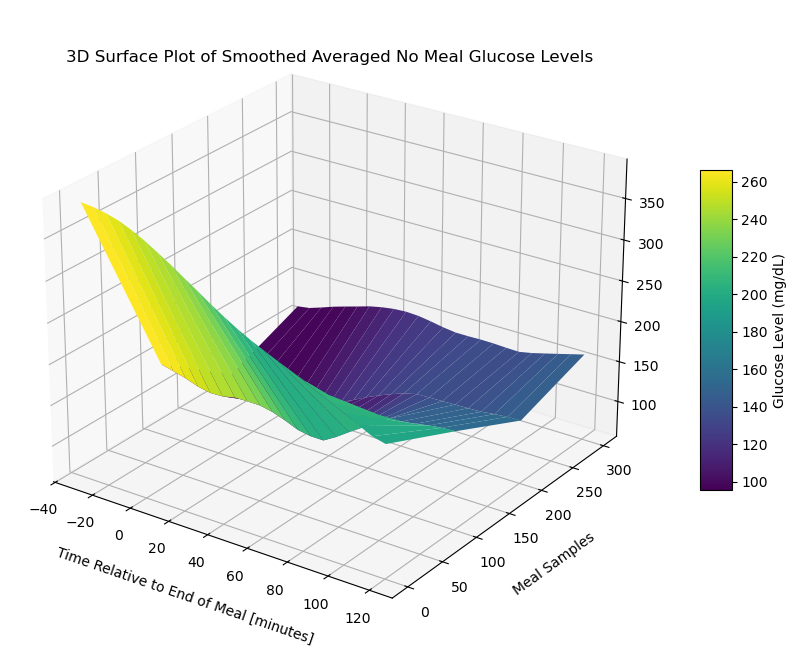
\includegraphics[width=0.7\linewidth]{files/53f8e67ddb84bce4df19d06f417ac1e8.png}

\subparagraph{Contour Plot of No Meal Data Matrix 2}

\begin{verbatim}
# Create the contour plot
plt.figure(figsize=(15, 10))
plt.contourf(X, Y, no_meal_data_matrix_2_df, cmap='viridis', levels=30)
plt.colorbar(label='Glucose Level (mg/dL)')
plt.title('Contour Plot of No Meal Glucose Levels')
plt.xlabel('Time Points')
plt.ylabel('Meal Samples')
plt.show()
\end{verbatim}

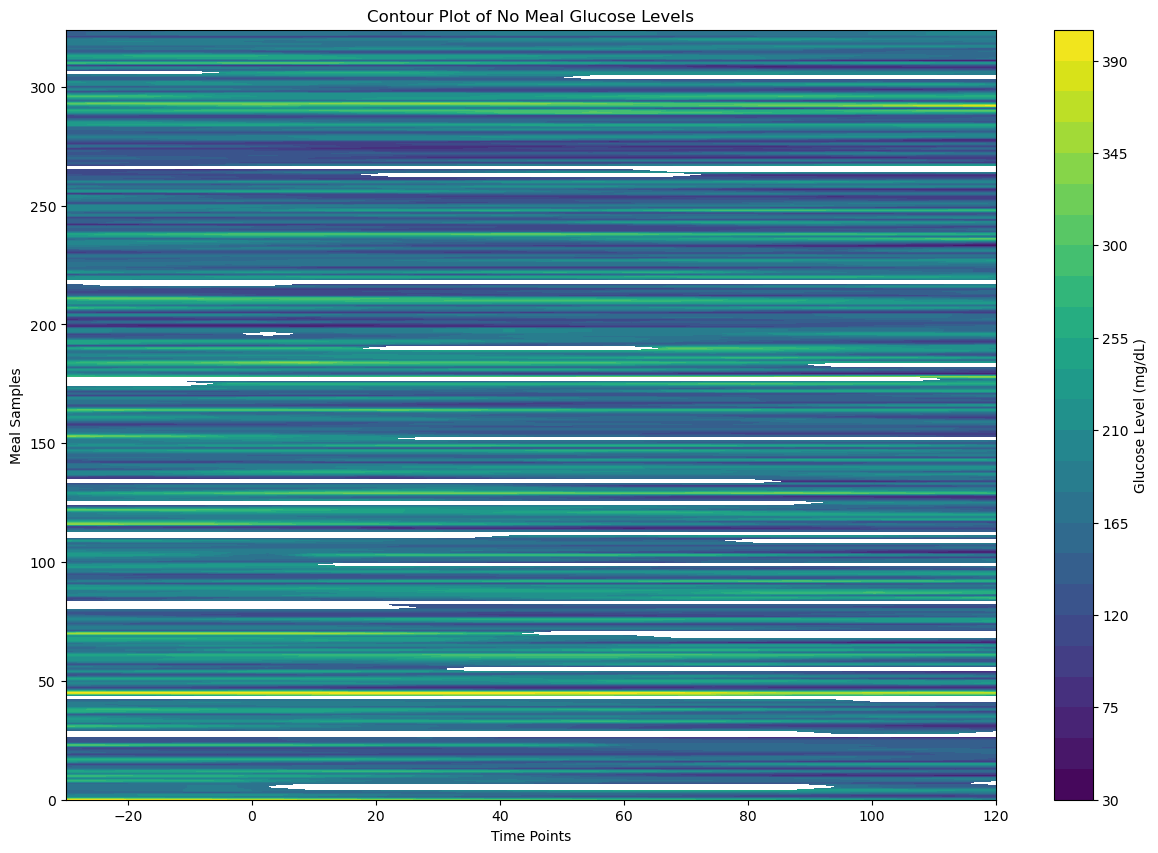
\includegraphics[width=0.7\linewidth]{files/51695a6d9698fcaf8b0a3f4f05b11c79.png}

\begin{verbatim}

\end{verbatim}

\subparagraph{Handle Missing Data}

We will use a strategy of deleting rows of data that have more than 10\% of bad data.  If less than 10\%, we will use KNN with a nearest neighbor hyperparameter (K=7).

\subparagraph{Define Threshold for Dumping Data}

\begin{verbatim}
# 10%
dump_thresold = 0.1
\end{verbatim}

\subparagraph{Create KNN Imputer}

\begin{verbatim}
knn_imputer = KNNImputer(n_neighbors=7)
\end{verbatim}

\subparagraph{Parse Meal Data and Handle Missing Values}

\begin{verbatim}
cleaned_meal_data_1 = []
for row in meal_data_matrix_1:

    proportion_missing_data = np.isnan(row).mean()

    if proportion_missing_data > dump_thresold:

        # Ignore this row
        print(f"Ignoring row with {proportion_missing_data*100:.2f}% missing data")
        continue

    else:
        # The data is good, use it
        cleaned_meal_data_1.append(row)
\end{verbatim}

\begin{verbatim}
Ignoring row with 13.33% missing data
Ignoring row with 73.33% missing data
Ignoring row with 66.67% missing data
Ignoring row with 13.33% missing data
Ignoring row with 30.00% missing data
Ignoring row with 16.67% missing data
Ignoring row with 23.33% missing data
Ignoring row with 16.67% missing data
Ignoring row with 26.67% missing data
Ignoring row with 30.00% missing data
Ignoring row with 20.00% missing data
Ignoring row with 73.33% missing data
Ignoring row with 63.33% missing data
Ignoring row with 100.00% missing data
Ignoring row with 100.00% missing data
Ignoring row with 33.33% missing data
Ignoring row with 16.67% missing data
Ignoring row with 16.67% missing data
Ignoring row with 100.00% missing data
Ignoring row with 60.00% missing data
Ignoring row with 16.67% missing data
Ignoring row with 36.67% missing data
Ignoring row with 43.33% missing data
Ignoring row with 13.33% missing data
Ignoring row with 13.33% missing data
Ignoring row with 60.00% missing data
Ignoring row with 16.67% missing data
Ignoring row with 53.33% missing data
Ignoring row with 33.33% missing data
Ignoring row with 13.33% missing data
Ignoring row with 20.00% missing data
Ignoring row with 83.33% missing data
Ignoring row with 86.67% missing data
Ignoring row with 70.00% missing data
Ignoring row with 16.67% missing data
Ignoring row with 100.00% missing data
Ignoring row with 100.00% missing data
Ignoring row with 16.67% missing data
Ignoring row with 43.33% missing data
Ignoring row with 100.00% missing data
Ignoring row with 100.00% missing data
Ignoring row with 63.33% missing data
Ignoring row with 63.33% missing data
Ignoring row with 26.67% missing data
Ignoring row with 60.00% missing data
Ignoring row with 100.00% missing data
Ignoring row with 100.00% missing data
Ignoring row with 33.33% missing data
Ignoring row with 96.67% missing data
Ignoring row with 100.00% missing data
Ignoring row with 100.00% missing data
Ignoring row with 100.00% missing data
Ignoring row with 20.00% missing data
Ignoring row with 80.00% missing data
Ignoring row with 43.33% missing data
Ignoring row with 100.00% missing data
Ignoring row with 16.67% missing data
Ignoring row with 100.00% missing data
Ignoring row with 70.00% missing data
Ignoring row with 16.67% missing data
Ignoring row with 83.33% missing data
Ignoring row with 83.33% missing data
Ignoring row with 30.00% missing data
Ignoring row with 16.67% missing data
Ignoring row with 100.00% missing data
Ignoring row with 20.00% missing data
Ignoring row with 30.00% missing data
Ignoring row with 20.00% missing data
Ignoring row with 76.67% missing data
Ignoring row with 73.33% missing data
Ignoring row with 70.00% missing data
Ignoring row with 36.67% missing data
Ignoring row with 20.00% missing data
Ignoring row with 16.67% missing data
Ignoring row with 36.67% missing data
Ignoring row with 16.67% missing data
Ignoring row with 63.33% missing data
Ignoring row with 13.33% missing data
Ignoring row with 20.00% missing data
Ignoring row with 26.67% missing data
Ignoring row with 90.00% missing data
Ignoring row with 23.33% missing data
Ignoring row with 33.33% missing data
Ignoring row with 100.00% missing data
Ignoring row with 80.00% missing data
Ignoring row with 33.33% missing data
Ignoring row with 30.00% missing data
Ignoring row with 20.00% missing data
Ignoring row with 33.33% missing data
Ignoring row with 100.00% missing data
Ignoring row with 100.00% missing data
Ignoring row with 13.33% missing data
Ignoring row with 20.00% missing data
Ignoring row with 100.00% missing data
Ignoring row with 100.00% missing data
Ignoring row with 16.67% missing data
\end{verbatim}

\begin{verbatim}
cleaned_meal_data_2 = []
for row in meal_data_matrix_2:

    proportion_missing_data = np.isnan(row).mean()

    if proportion_missing_data > dump_thresold:

        # Ignore this row
        print(f"Ignoring row with {proportion_missing_data*100:.2f}% missing data")
        continue

    else:
        # The data is good, use it
        cleaned_meal_data_2.append(row)
\end{verbatim}

\begin{verbatim}
Ignoring row with 43.33% missing data
Ignoring row with 43.33% missing data
Ignoring row with 30.00% missing data
Ignoring row with 63.33% missing data
Ignoring row with 36.67% missing data
Ignoring row with 100.00% missing data
Ignoring row with 66.67% missing data
Ignoring row with 26.67% missing data
Ignoring row with 100.00% missing data
Ignoring row with 56.67% missing data
Ignoring row with 53.33% missing data
Ignoring row with 70.00% missing data
Ignoring row with 20.00% missing data
Ignoring row with 16.67% missing data
Ignoring row with 20.00% missing data
Ignoring row with 100.00% missing data
Ignoring row with 100.00% missing data
Ignoring row with 16.67% missing data
Ignoring row with 13.33% missing data
Ignoring row with 100.00% missing data
Ignoring row with 60.00% missing data
Ignoring row with 80.00% missing data
Ignoring row with 36.67% missing data
Ignoring row with 100.00% missing data
Ignoring row with 56.67% missing data
Ignoring row with 63.33% missing data
Ignoring row with 20.00% missing data
Ignoring row with 20.00% missing data
Ignoring row with 26.67% missing data
Ignoring row with 13.33% missing data
Ignoring row with 73.33% missing data
Ignoring row with 36.67% missing data
Ignoring row with 23.33% missing data
Ignoring row with 13.33% missing data
Ignoring row with 13.33% missing data
Ignoring row with 13.33% missing data
Ignoring row with 36.67% missing data
Ignoring row with 100.00% missing data
Ignoring row with 26.67% missing data
Ignoring row with 26.67% missing data
Ignoring row with 100.00% missing data
Ignoring row with 20.00% missing data
Ignoring row with 20.00% missing data
Ignoring row with 16.67% missing data
Ignoring row with 16.67% missing data
Ignoring row with 20.00% missing data
Ignoring row with 20.00% missing data
\end{verbatim}

\begin{verbatim}
cleaned_meal_data_1[0]
\end{verbatim}

\begin{verbatim}
array([121., 120., 115., 110., 106., 103., 103., 101.,  nan, 131., 109.,
        82.,  74.,  66.,  73.,  82.,  87.,  90.,  83.,  73.,  49.,  58.,
        69.,  79.,  nan,  93.,  92.,  86.,  84.,  80.])
\end{verbatim}

\begin{verbatim}
cleaned_meal_data_2[0]
\end{verbatim}

\begin{verbatim}
array([390., 391., 389., 383., 375., 368., 357., 349., 336., 326., 315.,
       305., 295., 286., 279., 273., 268., 259., 252., 246., 238., 229.,
       218., 206., 195., 192., 181., 165., 139., 133.])
\end{verbatim}

\subparagraph{Convert Cleaned Meal Data List into a Matrix}

\begin{verbatim}
cleaned_meal_data_matrix_1 = \
    np.array(cleaned_meal_data_1)
\end{verbatim}

\begin{verbatim}
cleaned_meal_data_matrix_2 = \
    np.array(cleaned_meal_data_2)
\end{verbatim}

\subparagraph{Use KNN to Impute NaNs in Cleaned Meal Data}

\begin{verbatim}
cleaned_imputed_meal_matrix_1 = knn_imputer.fit_transform(cleaned_meal_data_matrix_1)
\end{verbatim}

\begin{verbatim}
cleaned_imputed_meal_matrix_2 = knn_imputer.fit_transform(cleaned_meal_data_matrix_2)
\end{verbatim}

\begin{verbatim}
cleaned_imputed_meal_matrix_1[0]
\end{verbatim}

\begin{verbatim}
array([121.        , 120.        , 115.        , 110.        ,
       106.        , 103.        , 103.        , 101.        ,
        99.71428571, 131.        , 109.        ,  82.        ,
        74.        ,  66.        ,  73.        ,  82.        ,
        87.        ,  90.        ,  83.        ,  73.        ,
        49.        ,  58.        ,  69.        ,  79.        ,
        75.85714286,  93.        ,  92.        ,  86.        ,
        84.        ,  80.        ])
\end{verbatim}

\begin{verbatim}
cleaned_imputed_meal_matrix_1.shape
\end{verbatim}

\begin{verbatim}
(619, 30)
\end{verbatim}

\begin{verbatim}
cleaned_imputed_meal_matrix_2[0]
\end{verbatim}

\begin{verbatim}
array([390., 391., 389., 383., 375., 368., 357., 349., 336., 326., 315.,
       305., 295., 286., 279., 273., 268., 259., 252., 246., 238., 229.,
       218., 206., 195., 192., 181., 165., 139., 133.])
\end{verbatim}

\begin{verbatim}
cleaned_imputed_meal_matrix_2.shape
\end{verbatim}

\begin{verbatim}
(325, 30)
\end{verbatim}

\subparagraph{Parse No Meal Data and Handle Missing Values}

\begin{verbatim}
cleaned_no_meal_data_1 = []
for row in no_meal_data_matrix_1:

    proportion_missing_data = np.isnan(row).mean()

    if proportion_missing_data > dump_thresold:

        # Ignore this row
        print(f"Ignoring row with {proportion_missing_data*100:.2f}% missing data")
        continue

    else:
        # The data is good, use it
        cleaned_no_meal_data_1.append(row)
\end{verbatim}

\begin{verbatim}
Ignoring row with 20.83% missing data
Ignoring row with 58.33% missing data
Ignoring row with 12.50% missing data
Ignoring row with 33.33% missing data
Ignoring row with 12.50% missing data
Ignoring row with 41.67% missing data
Ignoring row with 79.17% missing data
Ignoring row with 16.67% missing data
Ignoring row with 100.00% missing data
Ignoring row with 100.00% missing data
Ignoring row with 100.00% missing data
Ignoring row with 66.67% missing data
Ignoring row with 50.00% missing data
Ignoring row with 16.67% missing data
Ignoring row with 29.17% missing data
Ignoring row with 12.50% missing data
Ignoring row with 66.67% missing data
Ignoring row with 83.33% missing data
Ignoring row with 12.50% missing data
Ignoring row with 16.67% missing data
Ignoring row with 20.83% missing data
Ignoring row with 54.17% missing data
Ignoring row with 100.00% missing data
Ignoring row with 91.67% missing data
Ignoring row with 100.00% missing data
Ignoring row with 12.50% missing data
Ignoring row with 12.50% missing data
Ignoring row with 100.00% missing data
Ignoring row with 12.50% missing data
Ignoring row with 12.50% missing data
Ignoring row with 79.17% missing data
Ignoring row with 62.50% missing data
Ignoring row with 54.17% missing data
Ignoring row with 100.00% missing data
Ignoring row with 100.00% missing data
Ignoring row with 100.00% missing data
Ignoring row with 100.00% missing data
Ignoring row with 12.50% missing data
Ignoring row with 100.00% missing data
Ignoring row with 50.00% missing data
Ignoring row with 12.50% missing data
Ignoring row with 37.50% missing data
Ignoring row with 91.67% missing data
Ignoring row with 87.50% missing data
Ignoring row with 66.67% missing data
Ignoring row with 41.67% missing data
Ignoring row with 87.50% missing data
Ignoring row with 41.67% missing data
Ignoring row with 87.50% missing data
Ignoring row with 100.00% missing data
Ignoring row with 12.50% missing data
Ignoring row with 41.67% missing data
Ignoring row with 29.17% missing data
Ignoring row with 100.00% missing data
\end{verbatim}

\begin{verbatim}
cleaned_no_meal_data_2 = []
for row in no_meal_data_matrix_2:

    proportion_missing_data = np.isnan(row).mean()

    if proportion_missing_data > dump_thresold:

        # Ignore this row
        print(f"Ignoring row with {proportion_missing_data*100:.2f}% missing data")
        continue

    else:
        # The data is good, use it
        cleaned_no_meal_data_2.append(row)
\end{verbatim}

\begin{verbatim}
Ignoring row with 54.17% missing data
Ignoring row with 54.17% missing data
Ignoring row with 100.00% missing data
Ignoring row with 83.33% missing data
Ignoring row with 16.67% missing data
Ignoring row with 100.00% missing data
Ignoring row with 58.33% missing data
Ignoring row with 37.50% missing data
Ignoring row with 50.00% missing data
Ignoring row with 37.50% missing data
Ignoring row with 100.00% missing data
Ignoring row with 70.83% missing data
Ignoring row with 29.17% missing data
Ignoring row with 45.83% missing data
Ignoring row with 100.00% missing data
Ignoring row with 79.17% missing data
Ignoring row with 75.00% missing data
Ignoring row with 62.50% missing data
Ignoring row with 16.67% missing data
Ignoring row with 91.67% missing data
Ignoring row with 20.83% missing data
Ignoring row with 29.17% missing data
Ignoring row with 20.83% missing data
Ignoring row with 100.00% missing data
Ignoring row with 33.33% missing data
Ignoring row with 37.50% missing data
Ignoring row with 100.00% missing data
Ignoring row with 45.83% missing data
Ignoring row with 16.67% missing data
\end{verbatim}

\begin{verbatim}
cleaned_no_meal_data_1[0]
\end{verbatim}

\begin{verbatim}
array([121., 120., 115., 110., 106., 103., 103., 101.,  nan, 131., 109.,
        82.,  74.,  66.,  73.,  82.,  87.,  90.,  83.,  73.,  49.,  58.,
        69.,  79.])
\end{verbatim}

\begin{verbatim}
cleaned_no_meal_data_2[0]
\end{verbatim}

\begin{verbatim}
array([390., 391., 389., 383., 375., 368., 357., 349., 336., 326., 315.,
       305., 295., 286., 279., 273., 268., 259., 252., 246., 238., 229.,
       218., 206.])
\end{verbatim}

\begin{verbatim}
cleaned_no_meal_data_1[0].shape
\end{verbatim}

\begin{verbatim}
(24,)
\end{verbatim}

\begin{verbatim}
cleaned_no_meal_data_2[0].shape
\end{verbatim}

\begin{verbatim}
(24,)
\end{verbatim}

\subparagraph{Convert Cleaned No Meal Data List into a Matrix}

\begin{verbatim}
cleaned_no_meal_data_matrix_1 = \
    np.array(cleaned_no_meal_data_1)
\end{verbatim}

\begin{verbatim}
cleaned_no_meal_data_matrix_2 = \
    np.array(cleaned_no_meal_data_2)
\end{verbatim}

\subparagraph{Use KNN to Impute NaNs in Cleaned No Meal Data}

\begin{verbatim}
cleaned_imputed_no_meal_matrix_1 = knn_imputer.fit_transform(cleaned_no_meal_data_matrix_1)
\end{verbatim}

\begin{verbatim}
cleaned_imputed_no_meal_matrix_2 = knn_imputer.fit_transform(cleaned_no_meal_data_matrix_2)
\end{verbatim}

\begin{verbatim}
cleaned_imputed_no_meal_matrix_1[0]
\end{verbatim}

\begin{verbatim}
array([121.        , 120.        , 115.        , 110.        ,
       106.        , 103.        , 103.        , 101.        ,
       103.85714286, 131.        , 109.        ,  82.        ,
        74.        ,  66.        ,  73.        ,  82.        ,
        87.        ,  90.        ,  83.        ,  73.        ,
        49.        ,  58.        ,  69.        ,  79.        ])
\end{verbatim}

\begin{verbatim}
cleaned_imputed_no_meal_matrix_2[0]
\end{verbatim}

\begin{verbatim}
array([390., 391., 389., 383., 375., 368., 357., 349., 336., 326., 315.,
       305., 295., 286., 279., 273., 268., 259., 252., 246., 238., 229.,
       218., 206.])
\end{verbatim}

\subparagraph{Visualize Cleaned Imputed Data}

\subparagraph{Visualize Cleaned Imputed Meal Data Matrix 1}

\subparagraph{Heatmap of Cleaned Imputed Meal Data Matrix 1}

\begin{verbatim}
# Create the heatmap
sampled_meal_data_matrix_1 = cleaned_imputed_meal_matrix_1[np.random.choice(cleaned_imputed_meal_matrix_1.shape[0], 200, replace=False)]
plt.figure(figsize=(30, 30))
sns.heatmap(sampled_meal_data_matrix_1, cmap='YlGnBu', linewidths=0.5, annot=False, vmin=None, vmax=None)
plt.title('Heatmap of Meal Data Matrix 1', fontsize=30)
plt.xlabel('Time Points', fontsize=26)
plt.ylabel('Meals (Samples)', fontsize=26)

# Change font properties for the x and y tick labels
plt.xticks(fontsize=16)
plt.yticks(fontsize=16)

plt.show()
\end{verbatim}

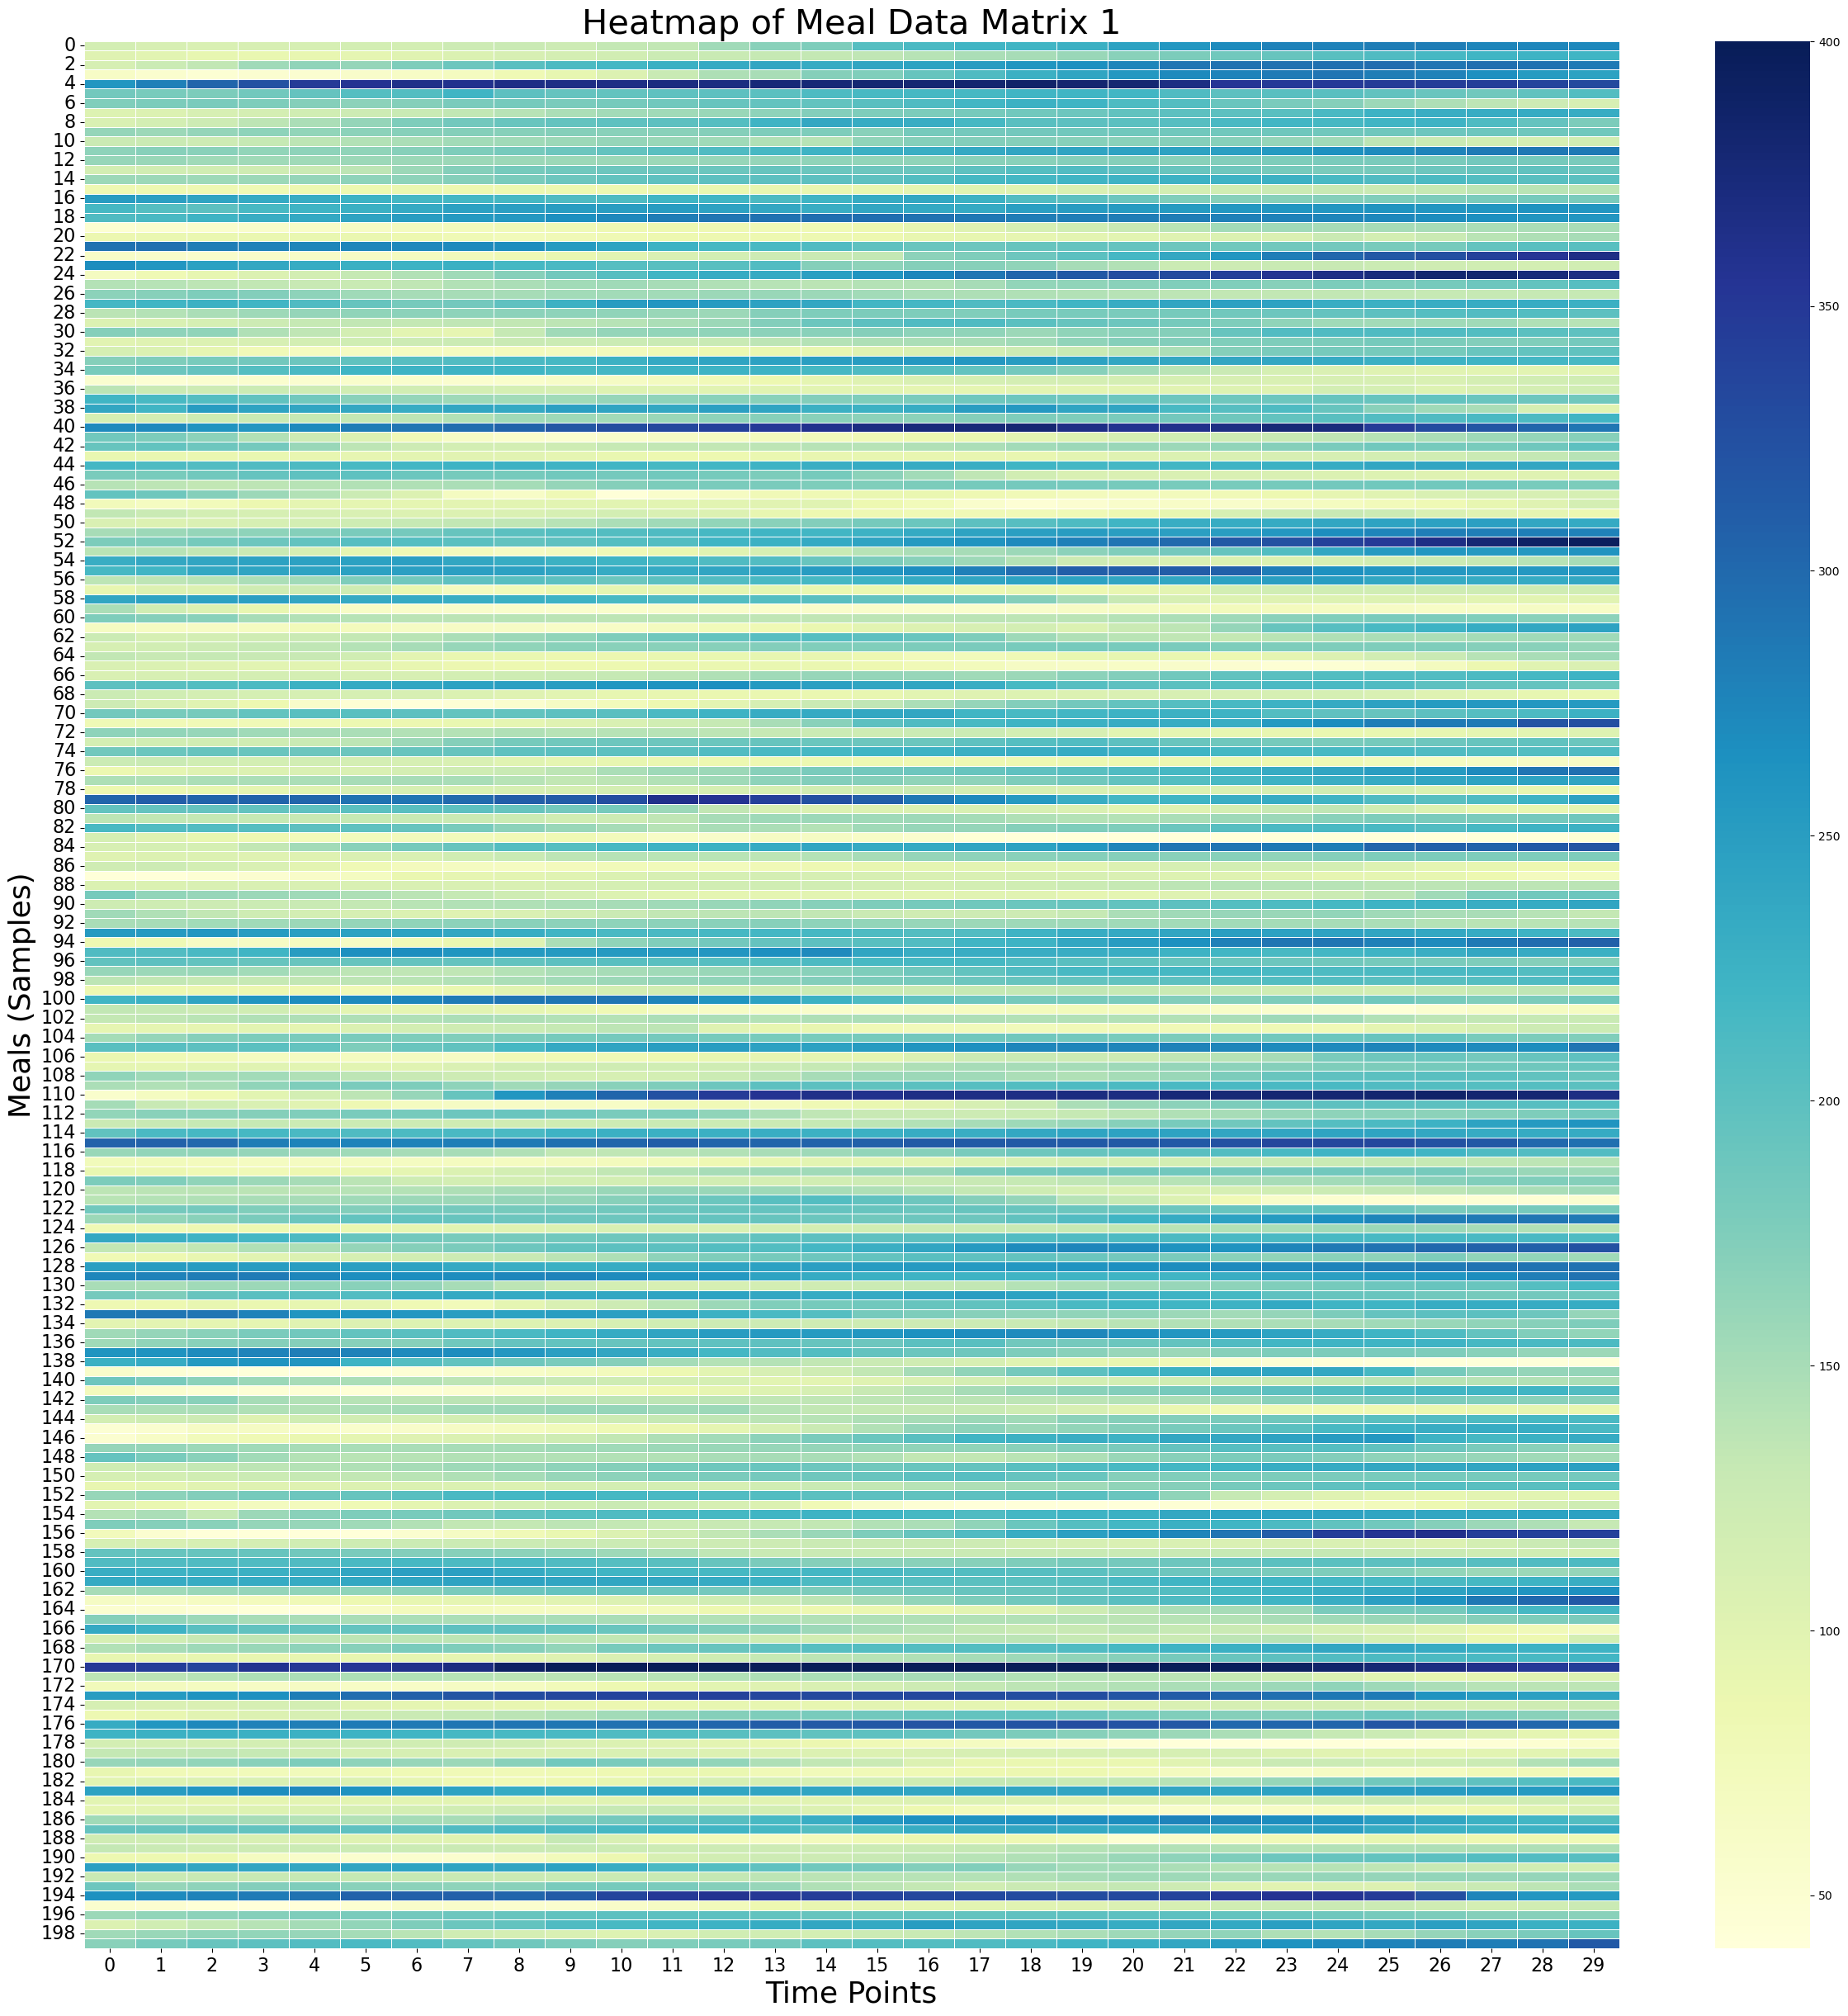
\includegraphics[width=0.7\linewidth]{files/afc0f68d7cc75c3160f17cbdfd91b534.png}

\subparagraph{Surface Plot of Cleaned Imputed Meal Data Matrix 1}

\begin{verbatim}
# Create X, Y meshgrid
X = np.arange(cleaned_imputed_meal_matrix_1.shape[1])
Y = np.arange(cleaned_imputed_meal_matrix_1.shape[0])
time_points = np.linspace( -30, 120, 30)  # X -axis: from -30 minutes to +120 minutes (30 time points)
meal_numbers = np.arange(1, len(meal_data_1) + 1)
X, Y = np.meshgrid(time_points, Y)
#X, Y = np.meshgrid(time_points, meal_numbers)
\end{verbatim}

\begin{verbatim}
X
\end{verbatim}

\begin{verbatim}
array([[ -30.        , -24.82758621, -19.65517241, ..., 109.65517241,
        114.82758621, 120.        ],
       [ -30.        , -24.82758621, -19.65517241, ..., 109.65517241,
        114.82758621, 120.        ],
       [ -30.        , -24.82758621, -19.65517241, ..., 109.65517241,
        114.82758621, 120.        ],
       ...,
       [ -30.        , -24.82758621, -19.65517241, ..., 109.65517241,
        114.82758621, 120.        ],
       [ -30.        , -24.82758621, -19.65517241, ..., 109.65517241,
        114.82758621, 120.        ],
       [ -30.        , -24.82758621, -19.65517241, ..., 109.65517241,
        114.82758621, 120.        ]])
\end{verbatim}

\begin{verbatim}
X.shape
\end{verbatim}

\begin{verbatim}
(619, 30)
\end{verbatim}

\begin{verbatim}
Y
\end{verbatim}

\begin{verbatim}
array([[  0,   0,   0, ...,   0,   0,   0],
       [  1,   1,   1, ...,   1,   1,   1],
       [  2,   2,   2, ...,   2,   2,   2],
       ...,
       [616, 616, 616, ..., 616, 616, 616],
       [617, 617, 617, ..., 617, 617, 617],
       [618, 618, 618, ..., 618, 618, 618]])
\end{verbatim}

\begin{verbatim}
# Fill NaNs using forward fill, then backward fill
meal_data_matrix_1_df = pd.DataFrame(cleaned_imputed_meal_matrix_1)
meal_data_matrix_1_filled = meal_data_matrix_1_df.ffill().bfill().values
\end{verbatim}

\begin{verbatim}
# Apply a moving average smoothing to each row
window_size = 3  # Choose a window size for smoothing
smoothed_meal_data_matrix_1 = np.array([uniform_filter1d(row, size=window_size) for row in meal_data_matrix_1_filled])
\end{verbatim}

\begin{verbatim}
# Create the plot
fig = plt.figure(figsize=(10, 8))
ax = fig.add_subplot(111, projection='3d')
stride = 100

# Plot the surface
surface_plot = ax.plot_surface(X[::stride], Y[::stride], smoothed_meal_data_matrix_1[::stride], cmap='viridis', edgecolor='none')
ax.set_title('3D Surface Plot of Smoothed Averaged Meal Glucose Levels', y=0.985)
ax.set_xlabel('Time Relative to Start of Meal [minutes]', labelpad=10)
ax.set_ylabel('Meal Samples', labelpad=10)
#ax.set_zlabel('Glucose Level (mg/dL)', labelpad=30)

#ax.set_xticks(np.linspace( -30, 120, 7))

# Adjust axis limits to create a zoom -out effect
#ax.set_xlim( -30, 120)
ax.set_ylim(0, 800)
ax.set_zlim(0, 300)

fig.colorbar(surface_plot, ax=ax, shrink=0.5, aspect=10, label='Glucose Level (mg/dL)')

#plt.tight_layout()
fig.subplots_adjust(left=0.01, right=1, top=0.9, bottom=0.1)

ax.view_init(elev=25, azim= -55)

plt.show()
\end{verbatim}

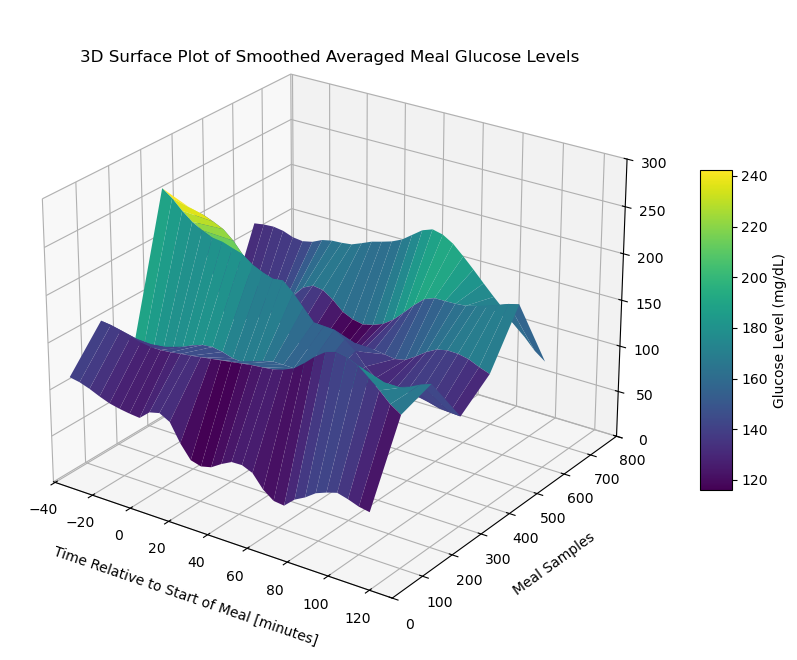
\includegraphics[width=0.7\linewidth]{files/8610e5d8597ff50c90111088edaf6301.png}

\subparagraph{Contour Plot of Cleaned Imputed Meal Data Matrix 1}

\begin{verbatim}
# Create the contour plot
plt.figure(figsize=(15, 10))
plt.contourf(X, Y, meal_data_matrix_1_df, cmap='viridis', levels=30)
plt.colorbar(label='Glucose Level (mg/dL)')
plt.title('Contour Plot of Meal Glucose Levels')
plt.xlabel('Time Points')
plt.ylabel('Meal Samples')
plt.show()
\end{verbatim}

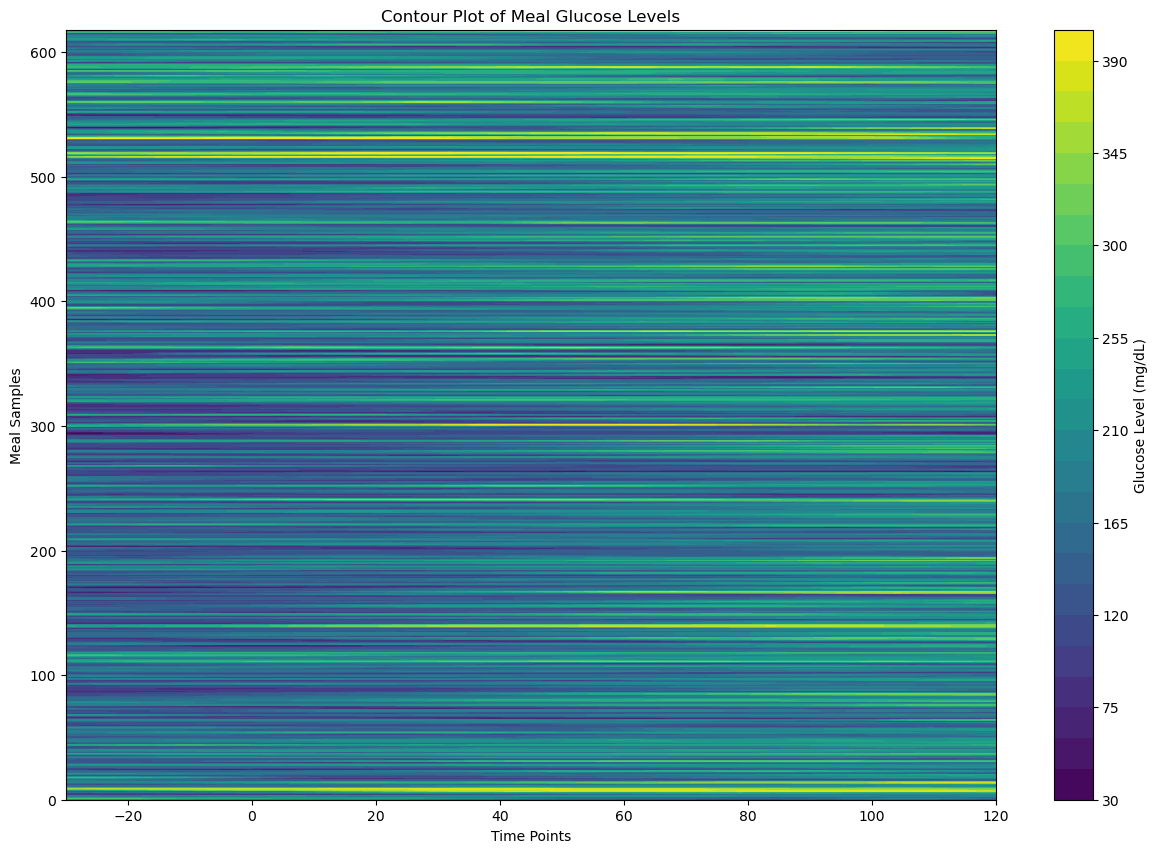
\includegraphics[width=0.7\linewidth]{files/8e605683861157585e3303ec82708e7f.png}

\subparagraph{Visualize Cleaned Imputed Meal Data Matrix 2}

\subparagraph{Heatmap of Cleaned Imputed Meal Data Matrix 2}

\begin{verbatim}
# Create the heatmap
sampled_meal_data_matrix_2 = cleaned_imputed_meal_matrix_1[np.random.choice(cleaned_imputed_meal_matrix_2.shape[0], 200, replace=False)]
plt.figure(figsize=(30, 30))
sns.heatmap(sampled_meal_data_matrix_2, cmap='YlGnBu', linewidths=0.5, annot=False, vmin=None, vmax=None)
plt.title('Heatmap of Meal Data Matrix 1')
plt.xlabel('Time Points')
plt.ylabel('Meals (Samples)')
plt.show()
\end{verbatim}

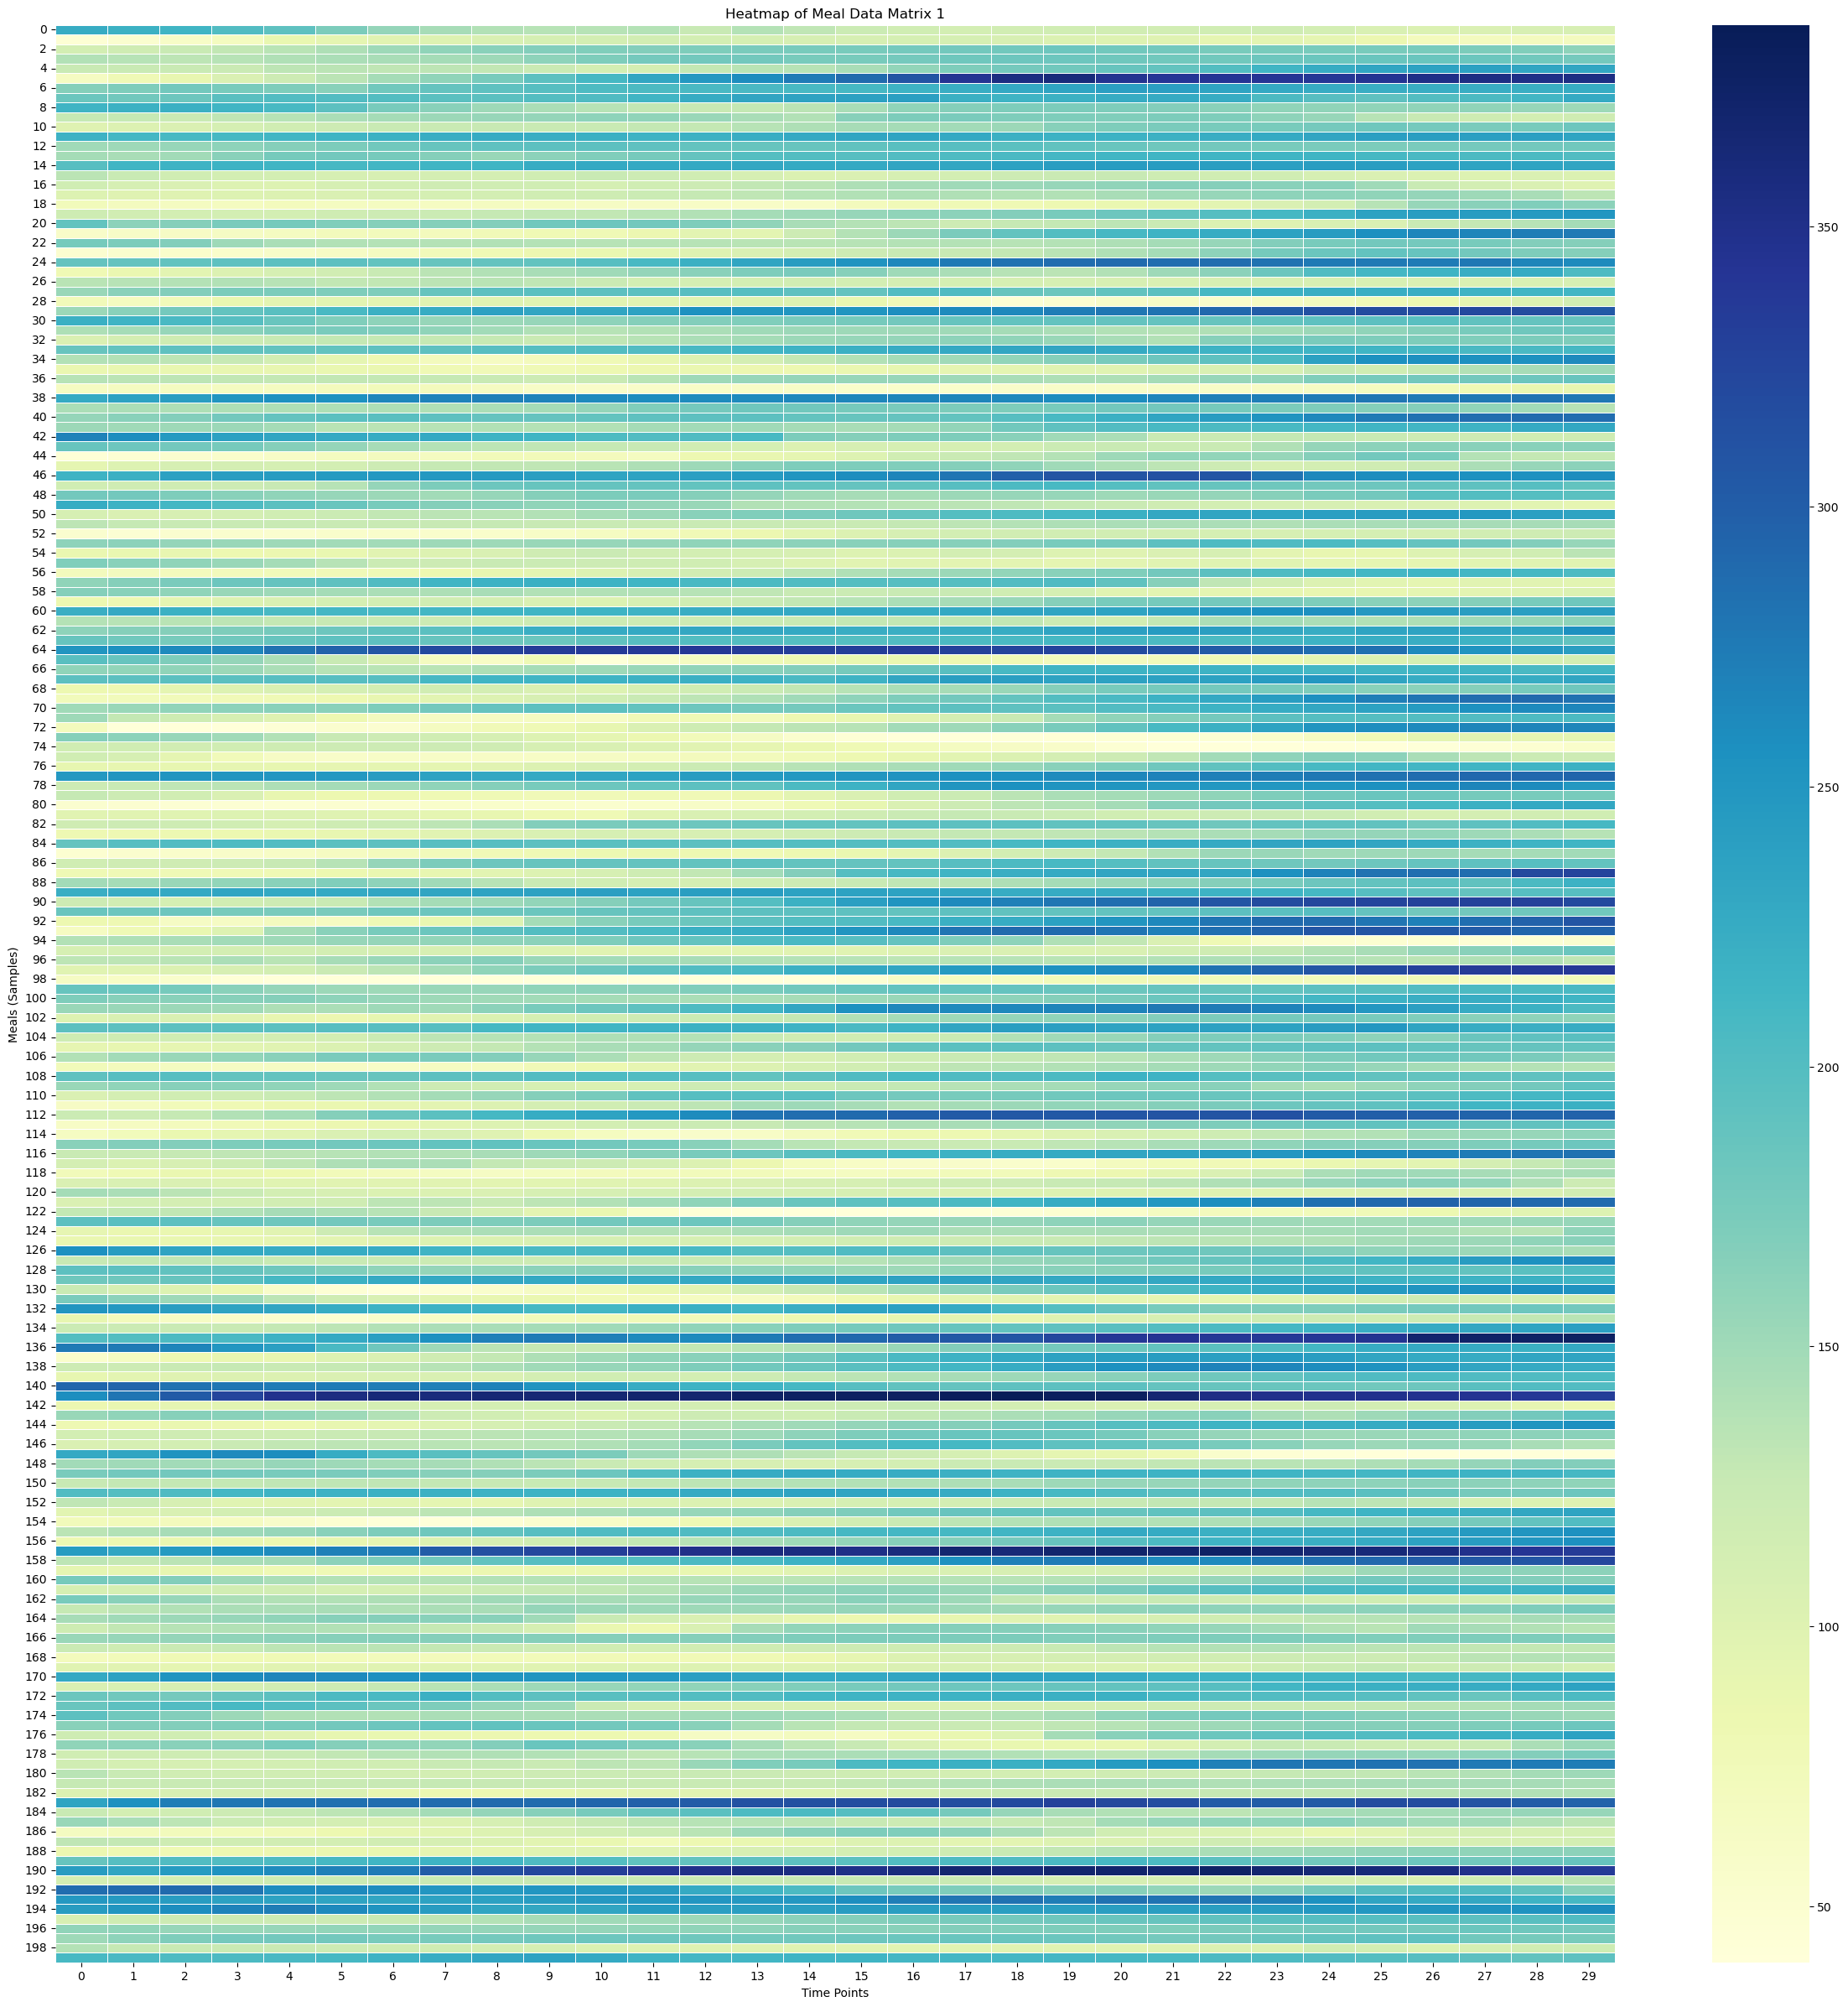
\includegraphics[width=0.7\linewidth]{files/1e0a4d3bdbd027698eb4faf198a9fae8.png}

\subparagraph{Surface Plot of Cleaned Imputed Meal Data Matrix 2}

\begin{verbatim}
# Create X, Y meshgrid
X = np.arange(cleaned_imputed_meal_matrix_2.shape[1])
Y = np.arange(cleaned_imputed_meal_matrix_2.shape[0])
time_points = np.linspace( -30, 120, 30)  # X -axis: from -30 minutes to +120 minutes (30 time points)
meal_numbers = np.arange(1, len(meal_data_2) + 1)
X, Y = np.meshgrid(time_points, Y)
#X, Y = np.meshgrid(time_points, meal_numbers)
\end{verbatim}

\begin{verbatim}
X
\end{verbatim}

\begin{verbatim}
array([[ -30.        , -24.82758621, -19.65517241, ..., 109.65517241,
        114.82758621, 120.        ],
       [ -30.        , -24.82758621, -19.65517241, ..., 109.65517241,
        114.82758621, 120.        ],
       [ -30.        , -24.82758621, -19.65517241, ..., 109.65517241,
        114.82758621, 120.        ],
       ...,
       [ -30.        , -24.82758621, -19.65517241, ..., 109.65517241,
        114.82758621, 120.        ],
       [ -30.        , -24.82758621, -19.65517241, ..., 109.65517241,
        114.82758621, 120.        ],
       [ -30.        , -24.82758621, -19.65517241, ..., 109.65517241,
        114.82758621, 120.        ]])
\end{verbatim}

\begin{verbatim}
X.shape
\end{verbatim}

\begin{verbatim}
(325, 30)
\end{verbatim}

\begin{verbatim}
Y
\end{verbatim}

\begin{verbatim}
array([[  0,   0,   0, ...,   0,   0,   0],
       [  1,   1,   1, ...,   1,   1,   1],
       [  2,   2,   2, ...,   2,   2,   2],
       ...,
       [322, 322, 322, ..., 322, 322, 322],
       [323, 323, 323, ..., 323, 323, 323],
       [324, 324, 324, ..., 324, 324, 324]])
\end{verbatim}

\begin{verbatim}
# Fill NaNs using forward fill, then backward fill
meal_data_matrix_2_df = pd.DataFrame(cleaned_imputed_meal_matrix_2)
meal_data_matrix_2_filled = meal_data_matrix_2_df.ffill().bfill().values
\end{verbatim}

\begin{verbatim}
# Apply a moving average smoothing to each row
window_size = 3  # Choose a window size for smoothing
smoothed_meal_data_matrix_2 = np.array([uniform_filter1d(row, size=window_size) for row in meal_data_matrix_2_filled])
\end{verbatim}

\begin{verbatim}
# Create the plot
fig = plt.figure(figsize=(10, 8))
ax = fig.add_subplot(111, projection='3d')
stride = 100

# Plot the surface
surface_plot = ax.plot_surface(X[::stride], Y[::stride], smoothed_meal_data_matrix_2[::stride], cmap='viridis', edgecolor='none')
ax.set_title('3D Surface Plot of Smoothed Averaged Meal Glucose Levels', y=0.985)
ax.set_xlabel('Time Relative to Start of Meal [minutes]', labelpad=10)
ax.set_ylabel('Meal Samples', labelpad=10)
#ax.set_zlabel('Glucose Level (mg/dL)', labelpad=30)

#ax.set_xticks(np.linspace( -30, 120, 7))

# Adjust axis limits to create a zoom -out effect
#ax.set_xlim( -30, 120)
#ax.set_ylim(0, 800)
#ax.set_zlim(0, 300)

fig.colorbar(surface_plot, ax=ax, shrink=0.5, aspect=10, label='Glucose Level (mg/dL)')

#plt.tight_layout()
fig.subplots_adjust(left=0.01, right=1, top=0.9, bottom=0.1)

ax.view_init(elev=25, azim= -55)

plt.show()
\end{verbatim}

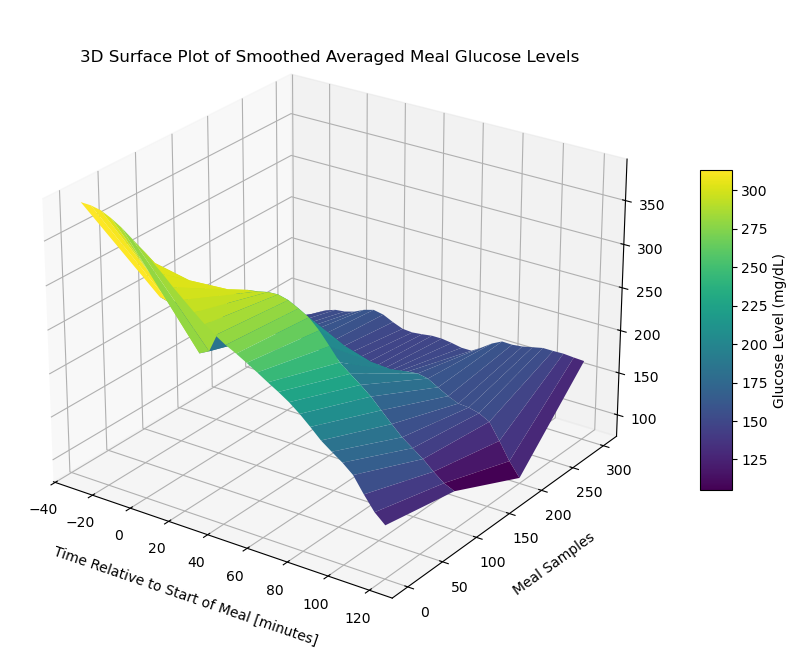
\includegraphics[width=0.7\linewidth]{files/a2c22604216cad76cf0e2eeeb83f600c.png}

\subparagraph{Contour Plot of Cleaned Imputed Meal Data Matrix 2}

\begin{verbatim}
# Create the contour plot
plt.figure(figsize=(15, 10))
plt.contourf(X, Y, meal_data_matrix_2_df, cmap='viridis', levels=30)
plt.colorbar(label='Glucose Level (mg/dL)')
plt.title('Contour Plot of Meal Glucose Levels')
plt.xlabel('Time Points')
plt.ylabel('Meal Samples')
plt.show()
\end{verbatim}

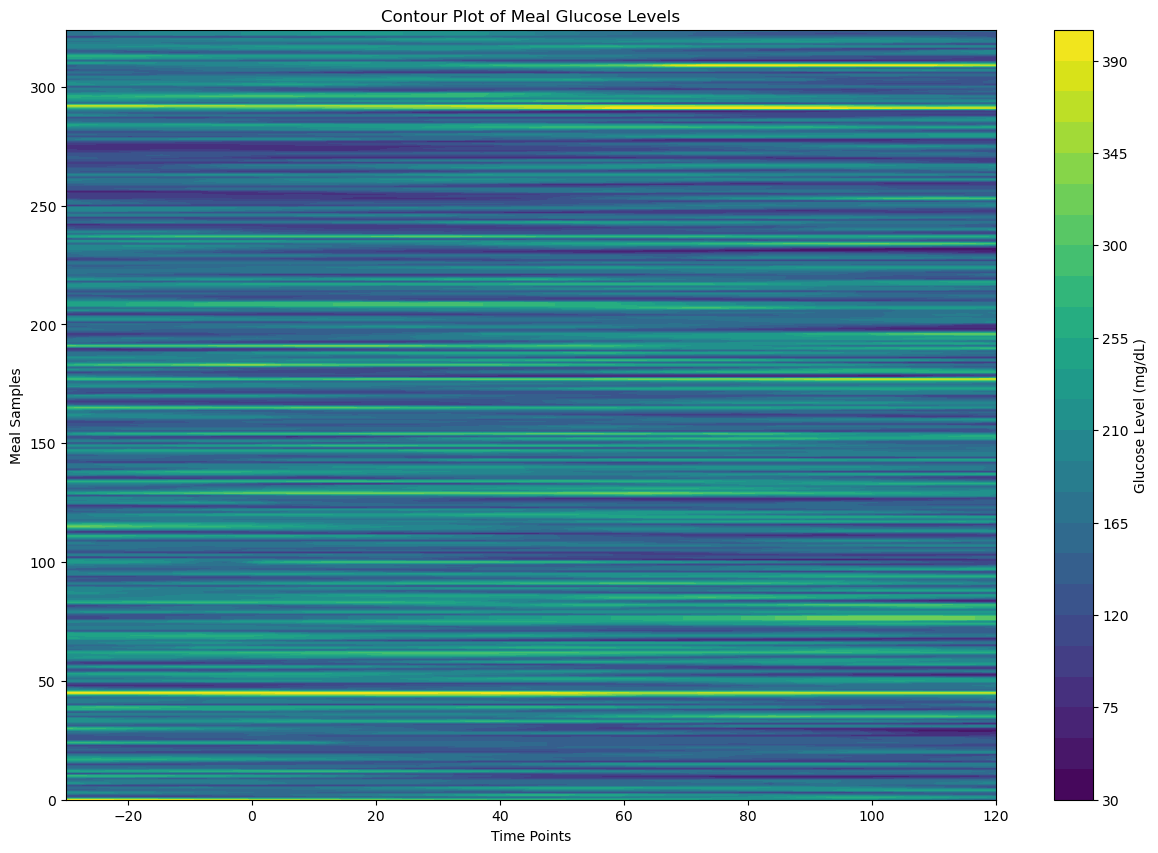
\includegraphics[width=0.7\linewidth]{files/819acd09172e4c3beb5adb998974033c.png}

\subparagraph{Combine Patient 1 and Patient 2 Data}

\begin{verbatim}
cleaned_imputed_meal_matrix = \
    np.vstack((cleaned_imputed_meal_matrix_1, cleaned_imputed_meal_matrix_2))
\end{verbatim}

\begin{verbatim}
cleaned_imputed_no_meal_matrix = \
    np.vstack((cleaned_imputed_no_meal_matrix_1, cleaned_imputed_no_meal_matrix_2))
\end{verbatim}

\subparagraph{Feature Extraction}

\subparagraph{Define Feature Extractor Helper Functions}

\begin{verbatim}
def compute_first_derivative(glucose_data, delta_t=5):
    return np.diff(glucose_data) / delta_t
\end{verbatim}

\begin{verbatim}
def compute_second_derivative(glucose_values, delta_t=5):
    second_derivative = np.zeros(len(glucose_values) - 2)
    for i in range(1, len(glucose_values) - 1):
        second_derivative[i - 1] = \
            (glucose_values[i + 1] - 2 * glucose_values[i] + glucose_values[i - 1]) / (delta_t ** 2)
    return second_derivative
\end{verbatim}

\begin{verbatim}
compute_first_derivative(cleaned_imputed_meal_matrix[0])
\end{verbatim}

\begin{verbatim}
array([ -0.2       , -1.        , -1.        , -0.8       , -0.6       ,
        0.        , -0.4       , -0.25714286,  6.25714286, -4.4       ,
       -5.4       , -1.6       , -1.6       ,  1.4       ,  1.8       ,
        1.        ,  0.6       , -1.4       , -2.        , -4.8       ,
        1.8       ,  2.2       ,  2.        , -0.62857143,  3.42857143,
       -0.2       , -1.2       , -0.4       , -0.8       ])
\end{verbatim}

\begin{verbatim}
compute_second_derivative(cleaned_imputed_meal_matrix[0])
\end{verbatim}

\begin{verbatim}
array([ -0.16      ,  0.        ,  0.04      ,  0.04      ,  0.12      ,
       -0.08      ,  0.02857143,  1.30285714, -2.13142857, -0.2       ,
        0.76      ,  0.        ,  0.6       ,  0.08      , -0.16      ,
       -0.08      , -0.4       , -0.12      , -0.56      ,  1.32      ,
        0.08      , -0.04      , -0.52571429,  0.81142857, -0.72571429,
       -0.2       ,  0.16      , -0.08      ])
\end{verbatim}

\begin{verbatim}
def compute_AUC(glucose_values, delta_t=5):
    return simpson(glucose_values, dx=delta_t)
\end{verbatim}

\subparagraph{Define Feature Extractor Function}

\begin{verbatim}
def feature_extractor(data_matrix):

    features = []

    for row in data_matrix:
        mean_glucose = np.mean(row)
        std_glucose  = np.std(row)
        max_glucose  = np.max(row)
        min_glucose  = np.min(row)
        
        first_derivative = compute_first_derivative(row)
        mean_first_derivate = np.mean(first_derivative)

        if len(row) > 2:
            second_derivative = compute_second_derivative(row)
            mean_second_derivative = np.mean(second_derivative)
        else:
            mean_second_derivative = 0

        AUC = compute_AUC(row)

        time_to_peak = np.argmax(row)

        features_vector = [
            mean_glucose,
            std_glucose,
            max_glucose,
            min_glucose,
            mean_first_derivate,
            mean_second_derivative,
            AUC,
            time_to_peak
        ]

        features.append(features_vector)
    
    return np.array(features)
\end{verbatim}

\subparagraph{Get Feature Matrix for Cleaned Imputed Meal Data}

\begin{verbatim}
meal_features_matrix = feature_extractor(cleaned_imputed_meal_matrix)
meal_features_matrix[0]
\end{verbatim}

\begin{verbatim}
array([ 8.98190476e+01,  1.91175360e+01,  1.31000000e+02,  4.90000000e+01,
       -2.82758621e -01, -4.28571429e -03,  1.30310714e+04,  9.00000000e+00])
\end{verbatim}

\subparagraph{Get Feature Matrix for Clean Imputed No Meal Data}

\begin{verbatim}
no_meal_features_matrix = feature_extractor(cleaned_imputed_no_meal_matrix)
no_meal_features_matrix[0]
\end{verbatim}

\begin{verbatim}
array([ 9.11607143e+01,  2.10808822e+01,  1.31000000e+02,  4.90000000e+01,
       -3.65217391e -01,  2.00000000e -02,  1.04699405e+04,  9.00000000e+00])
\end{verbatim}

\subparagraph{Visualize The Meal Features Matrix}

\subparagraph{Normalize The Data}

\begin{verbatim}
scaler = StandardScaler()
scaled_meal_features_matrix = scaler.fit_transform(meal_features_matrix)
scaled_no_meal_features_matrix = scaler.fit_transform(no_meal_features_matrix)
\end{verbatim}

\begin{verbatim}
scaled_meal_features_matrix[0]
\end{verbatim}

\begin{verbatim}
array([ -1.43931653, -0.6890434 , -1.43186426, -1.35409331, -0.73789252,
       -0.2568468 , -1.42698567, -0.72547238])
\end{verbatim}

\begin{verbatim}
scaled_no_meal_features_matrix[0]
\end{verbatim}

\begin{verbatim}
array([ -1.24861858, -0.24758492, -1.16121642, -1.39218291, -0.66468096,
        1.06439767, -1.24077771, -0.41467362])
\end{verbatim}

\subparagraph{Plot Features for all Rows}

\begin{verbatim}
meal_features_matrix.shape[0]
\end{verbatim}

\begin{verbatim}
944
\end{verbatim}

\begin{verbatim}
X = np.arange(
        start=0,
        stop=meal_features_matrix.shape[0]
    )
\end{verbatim}

\subparagraph{Plot Max, Mean, Min, and Std Dev for All Rows}

\begin{verbatim}
Y_mean = meal_features_matrix[:, 0] # First column
Y_mean_peaks, _ = find_peaks(Y_mean, height=20)

Y_mean_peaks_times = X[Y_mean_peaks]
Y_mean_peaks_values = Y_mean[Y_mean_peaks]

window_size = 3
Y_mean_peaks_moving_avg = np.convolve(Y_mean_peaks_values, np.ones(window_size)/window_size, mode='valid')
\end{verbatim}

\begin{verbatim}
Y_std = meal_features_matrix[:, 1] # Second column
\end{verbatim}

\begin{verbatim}
Y_max = meal_features_matrix[:, 2] # Third column
Y_max_peaks, _ = find_peaks(Y_max, height=20)

Y_max_peaks_times = X[Y_max_peaks]
Y_max_peaks_values = Y_max[Y_max_peaks]

window_size = 3
Y_max_peaks_moving_avg = np.convolve(Y_max_peaks_values, np.ones(window_size)/window_size, mode='valid')
\end{verbatim}

\begin{verbatim}
Y_max_peaks_times.shape
\end{verbatim}

\begin{verbatim}
(289,)
\end{verbatim}

\begin{verbatim}
Y_max_peaks_moving_avg.shape
\end{verbatim}

\begin{verbatim}
(287,)
\end{verbatim}

\begin{verbatim}
Y_min = meal_features_matrix[:, 3] # Fourth column
Y_min_peaks, _ = find_peaks(Y_min, height=20)

Y_min_peaks_times = X[Y_min_peaks]
Y_min_peaks_values = Y_min[Y_min_peaks]

window_size = 3
Y_min_peaks_moving_avg = np.convolve(Y_min_peaks_values, np.ones(window_size)/window_size, mode='valid')
\end{verbatim}

\begin{verbatim}
Y_min_peaks_moving_avg.shape
\end{verbatim}

\begin{verbatim}
(281,)
\end{verbatim}

\begin{verbatim}
# Create the plot
fig = plt.figure(figsize=(18, 6))
ax = fig.add_subplot(111)
stride = 5

# Plot the features
#ax.plot(X[::stride], Y_max[::stride], 'x', label='Max', color='red')
ax.plot(Y_max_peaks_times[:len(Y_max_peaks_moving_avg)], Y_max_peaks_moving_avg, color='red', label='Moving Average of Max', linewidth=2)

#ax.plot(X[::stride], Y_mean[::stride], label='Mean', color='blue')
ax.plot(Y_mean_peaks_times[:len(Y_mean_peaks_moving_avg)], Y_mean_peaks_moving_avg, color='blue', label='Moving Average of Mean', linewidth=2)

#ax.plot(X[::stride], Y_min[::stride], 'x', label='Min')
ax.plot(Y_min_peaks_times[:len(Y_min_peaks_moving_avg)], Y_min_peaks_moving_avg, color='green', label='Moving Average of Min', linewidth=2)

ax.plot(X[::stride], Y_std[::stride], label='Std Dev')

ax.set_title('Meal Glucose Level Features vs Data Row Number', fontsize=20)
ax.set_xlabel('Data Row Number [arbitrary] ', fontsize=16)
ax.set_ylabel('Glucose Level [mg/dL]', fontsize=16)

ax.set_xticks(np.linspace(0, 1000, 11))
ax.set_yticks(np.linspace(0, 400, 7))
ax.set_xlim( -50, 1000)
ax.set_ylim(0, 420)

#ax.text(300, 380, f'Viewing every {stride} rows')

# Adjust axis limits to create a zoom -out effect
#ax.set_xlim( -30, 120)
#ax.set_ylim(0, 800)

#plt.tight_layout()

plt.legend()

plt.show()
\end{verbatim}

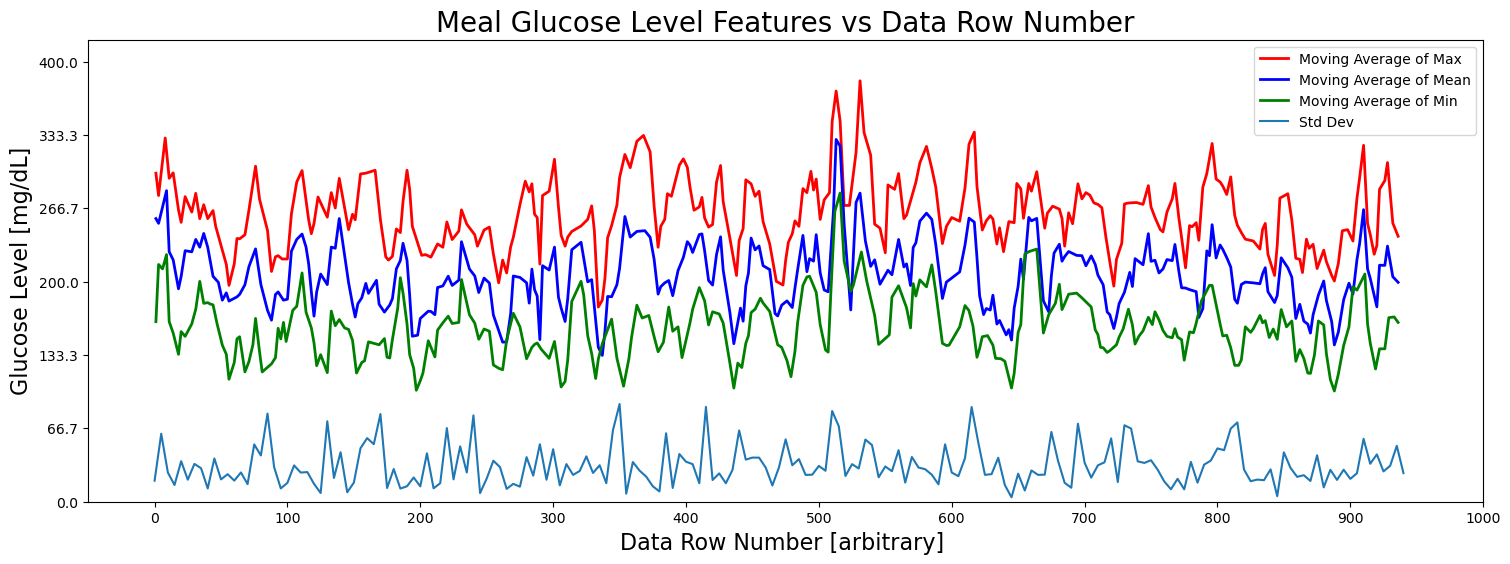
\includegraphics[width=0.7\linewidth]{files/b266108f8706ef7f3388009464603aef.png}

\subparagraph{Plot First and Second Derivatives}

\begin{verbatim}
Y_mean_first_derivative = meal_features_matrix[:, 4] # Fourth column
Y_mean_first_derivative_peaks, _ = find_peaks(Y_mean_first_derivative, height=None)

Y_mean_first_derivative_times = X[Y_mean_first_derivative_peaks]
Y_mean_first_derivative_values = Y_mean_first_derivative[Y_mean_first_derivative_peaks]

window_size = 3
Y_mean_first_derivative_peaks_moving_avg = \
    np.convolve(
        Y_mean_first_derivative_values,
        np.ones(window_size)/window_size, mode='valid'
    )
\end{verbatim}

\begin{verbatim}
Y_mean_2nd_derivative = meal_features_matrix[:, 5] # Fourth column
Y_mean_2nd_derivative_peaks, _ = find_peaks(Y_mean_2nd_derivative, height=None)

Y_mean_2nd_derivative_times = X[Y_mean_2nd_derivative_peaks]
Y_mean_2nd_derivative_values = Y_mean_2nd_derivative[Y_mean_2nd_derivative_peaks]

window_size = 3
Y_mean_2nd_derivative_peaks_moving_avg = \
    np.convolve(
        Y_mean_2nd_derivative_values,
        np.ones(window_size)/window_size, mode='valid'
    )
\end{verbatim}

\begin{verbatim}
# Create the plot
fig = plt.figure(figsize=(18, 6))
ax = fig.add_subplot(111)
stride = 5

# Plot the features
#ax.plot(X[::stride], Y_max[::stride], 'x', label='Max', color='red')
#ax.plot(
#    Y_max_peaks_times[:len(Y_max_peaks_moving_avg)], 
#    Y_max_peaks_moving_avg, 
#    color='red', 
#    label='Moving Average of Max', 
#    linewidth=2)

#ax.plot(X[::stride], Y_mean[::stride], label='Mean', color='blue')
ax.plot(
    Y_mean_peaks_times[:len(Y_mean_peaks_moving_avg)], 
    Y_mean_peaks_moving_avg, 
    color='blue', 
    label='Moving Average of Mean', 
    linewidth=2
)

#ax.plot(X[::stride], Y_min[::stride], 'x', label='Min')
#ax.plot(Y_min_peaks_times[:len(Y_min_peaks_moving_avg)], Y_min_peaks_moving_avg, color='green', label='Moving Average of Min', linewidth=2)

#ax.plot(X[::stride], Y_std[::stride], label='Std Dev')

ax.plot(
    Y_mean_first_derivative_times[:len(Y_mean_first_derivative_peaks_moving_avg)],
    Y_mean_first_derivative_peaks_moving_avg*100,
    color='orange',
    label=r'First Derivative $\times 100$',
    linewidth=2
)

ax.plot(
    Y_mean_2nd_derivative_times[:len(Y_mean_2nd_derivative_peaks_moving_avg)],
    Y_mean_2nd_derivative_peaks_moving_avg*2500,
    color='green',
    label=r'Second Derivative $\times 2500$',
    linewidth=2
)

ax.set_title('Glucose Level Features vs Data Row Number')
ax.set_xlabel('Data Row Number [arbitrary] ')
ax.set_ylabel('Glucose Level [mg/dL]')

#ax.set_xticks(np.linspace(0, 1000, 11))
#ax.set_yticks(np.linspace(0, 400, 7))
#ax.set_xlim( -50, 1000)
#ax.set_ylim(0, 420)

#ax.text(300, 380, f'Viewing every {stride} rows')

# Adjust axis limits to create a zoom -out effect
#ax.set_xlim( -30, 120)
#ax.set_ylim(0, 800)

#plt.tight_layout()

plt.legend()

plt.show()
\end{verbatim}

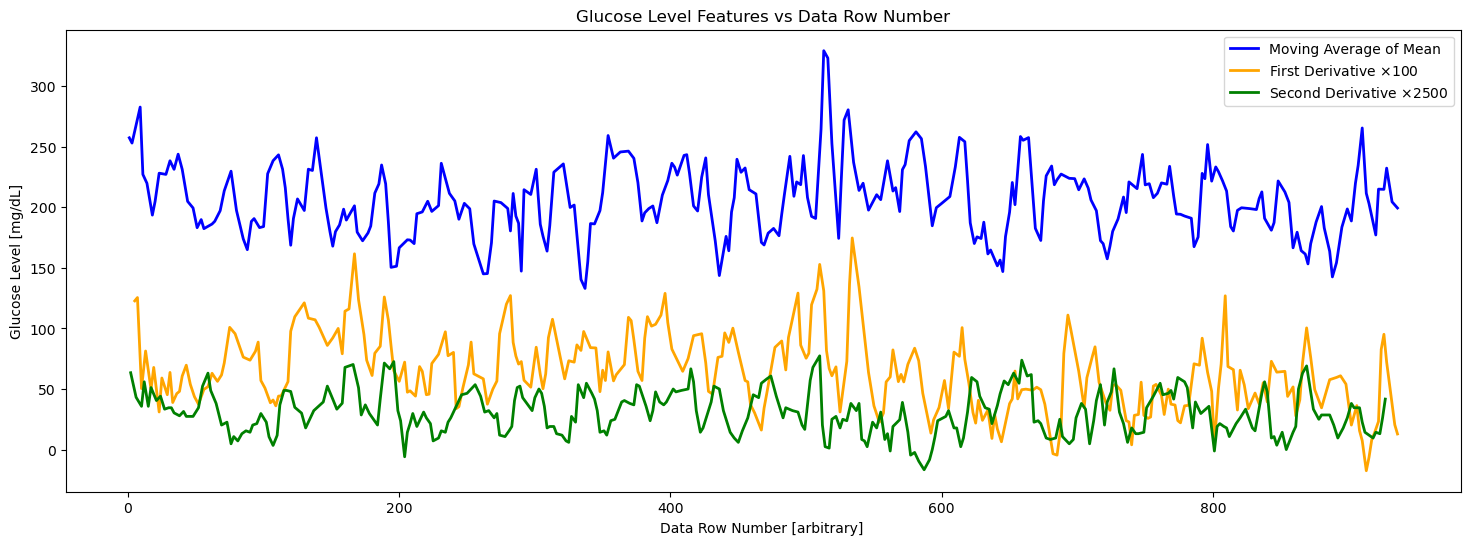
\includegraphics[width=0.7\linewidth]{files/d893bad643ecbad09dc4a751c436cb24.png}

\subparagraph{Pairwise Plot of Meal Features Matrix}

\begin{verbatim}
# Generate column labels for the features
feature_columns = [f'Feature_{i+1}' for i in range(meal_features_matrix.shape[1])]

# Convert the feature matrix to a Pandas DataFrame
df = pd.DataFrame(meal_features_matrix, columns=feature_columns)

# Create a pairwise plot using Seaborn
plt.figure(figsize=(15, 15))  # Adjust figure size as needed
sns.pairplot(df, diag_kind='hist', plot_kws={'alpha': 0.5, 's': 40})

plt.suptitle('Pairwise Plot of Meal Features Matrix', y=1.02, fontsize=30)

# Show the plot
plt.show()
\end{verbatim}

\begin{verbatim}
<Figure size 1500x1500 with 0 Axes>
\end{verbatim}

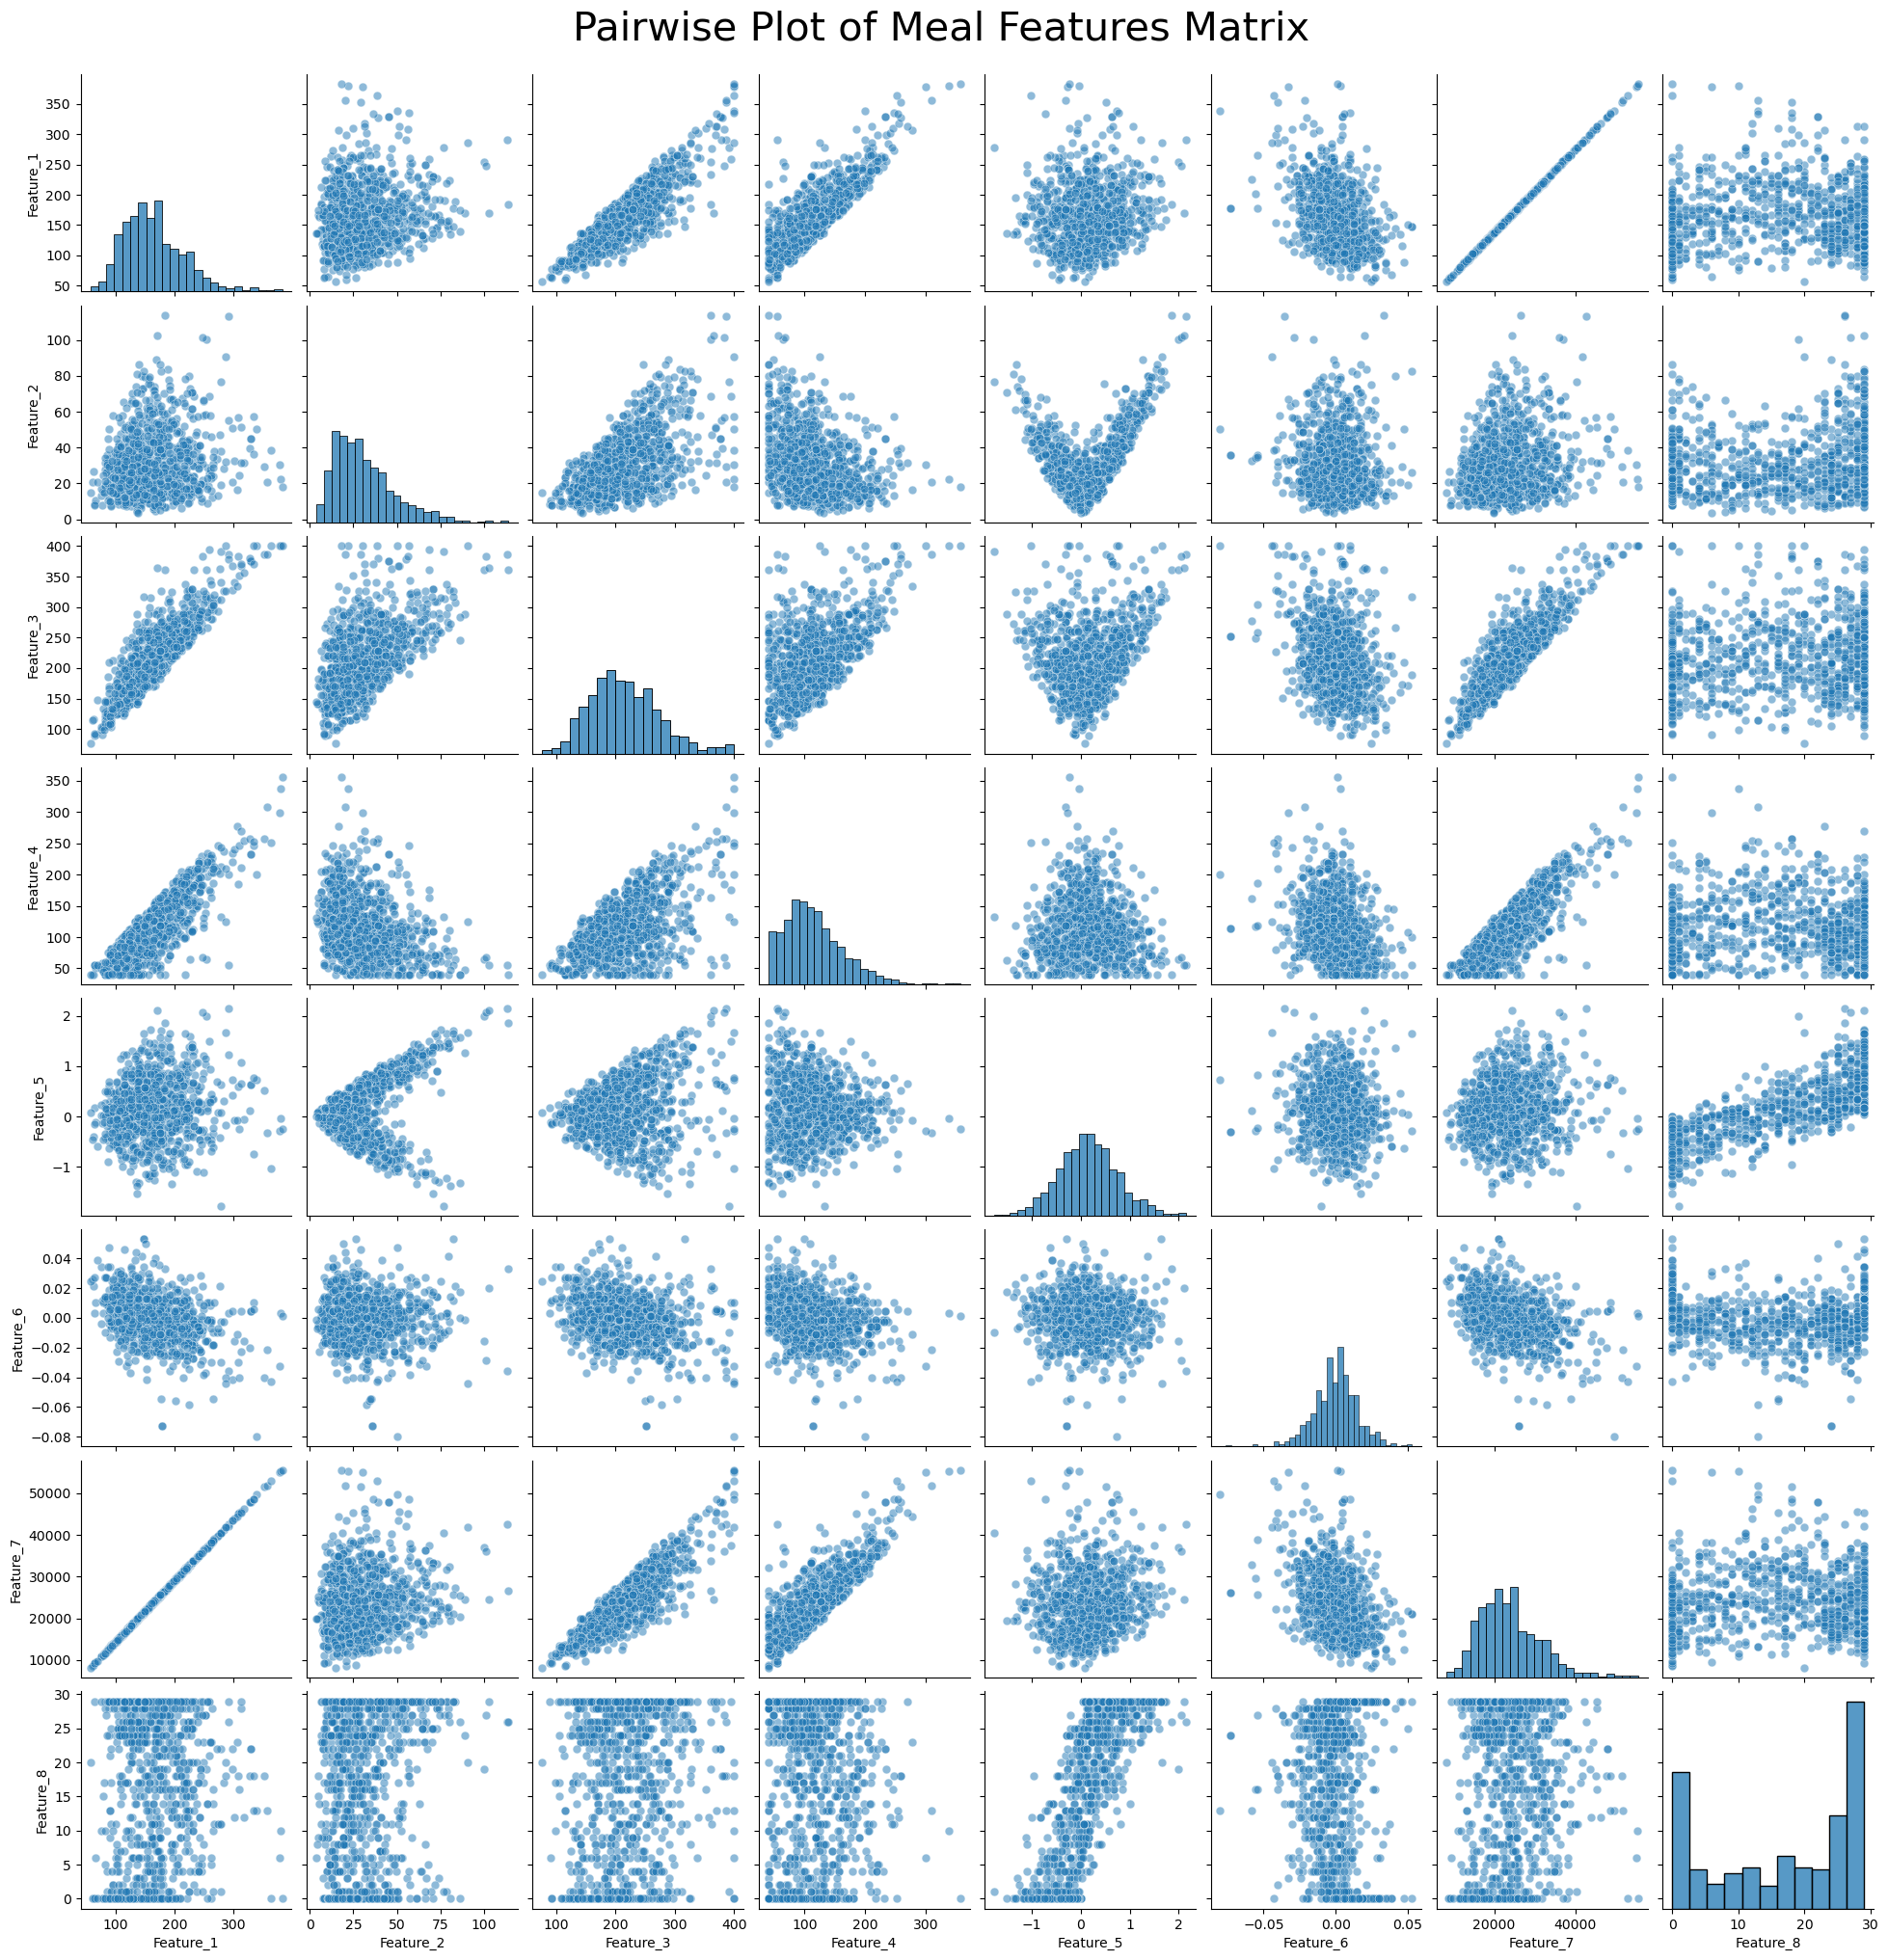
\includegraphics[width=0.7\linewidth]{files/f62ec84e21461b12e74a7631bac6bc54.png}

\subparagraph{Visualize The No Meal Features Matrix}

\subparagraph{Normalize The Data}

\begin{verbatim}
scaler = StandardScaler()
scaled_meal_features_matrix = scaler.fit_transform(meal_features_matrix)
scaled_no_meal_features_matrix = scaler.fit_transform(no_meal_features_matrix)
\end{verbatim}

\begin{verbatim}
scaled_meal_features_matrix[0]
\end{verbatim}

\begin{verbatim}
array([ -1.43931653, -0.6890434 , -1.43186426, -1.35409331, -0.73789252,
       -0.2568468 , -1.42698567, -0.72547238])
\end{verbatim}

\begin{verbatim}
scaled_no_meal_features_matrix[0]
\end{verbatim}

\begin{verbatim}
array([ -1.24861858, -0.24758492, -1.16121642, -1.39218291, -0.66468096,
        1.06439767, -1.24077771, -0.41467362])
\end{verbatim}

\subparagraph{Plot Features for all Rows}

\begin{verbatim}
no_meal_features_matrix.shape[0]
\end{verbatim}

\begin{verbatim}
752
\end{verbatim}

\begin{verbatim}
X = np.arange(
        start=0,
        stop=no_meal_features_matrix.shape[0]
    )
\end{verbatim}

\subparagraph{Plot Max, Mean, Min, and Std Dev for All Rows}

\begin{verbatim}
Y_mean = no_meal_features_matrix[:, 0] # First column
Y_mean_peaks, _ = find_peaks(Y_mean, height=20)

Y_mean_peaks_times = X[Y_mean_peaks]
Y_mean_peaks_values = Y_mean[Y_mean_peaks]

window_size = 3
Y_mean_peaks_moving_avg = np.convolve(Y_mean_peaks_values, np.ones(window_size)/window_size, mode='valid')
\end{verbatim}

\begin{verbatim}
Y_std = no_meal_features_matrix[:, 1] # Second column
\end{verbatim}

\begin{verbatim}
Y_max = no_meal_features_matrix[:, 2] # Third column
Y_max_peaks, _ = find_peaks(Y_max, height=20)

Y_max_peaks_times = X[Y_max_peaks]
Y_max_peaks_values = Y_max[Y_max_peaks]

window_size = 3
Y_max_peaks_moving_avg = np.convolve(Y_max_peaks_values, np.ones(window_size)/window_size, mode='valid')
\end{verbatim}

\begin{verbatim}
Y_max_peaks_times.shape
\end{verbatim}

\begin{verbatim}
(238,)
\end{verbatim}

\begin{verbatim}
Y_max_peaks_moving_avg.shape
\end{verbatim}

\begin{verbatim}
(236,)
\end{verbatim}

\begin{verbatim}
Y_min = no_meal_features_matrix[:, 3] # Fourth column
Y_min_peaks, _ = find_peaks(Y_min, height=20)

Y_min_peaks_times = X[Y_min_peaks]
Y_min_peaks_values = Y_min[Y_min_peaks]

window_size = 3
Y_min_peaks_moving_avg = np.convolve(Y_min_peaks_values, np.ones(window_size)/window_size, mode='valid')
\end{verbatim}

\begin{verbatim}
Y_min_peaks_moving_avg.shape
\end{verbatim}

\begin{verbatim}
(238,)
\end{verbatim}

\begin{verbatim}
# Create the plot
fig = plt.figure(figsize=(18, 6))
ax = fig.add_subplot(111)
stride = 5

# Plot the features
#ax.plot(X[::stride], Y_max[::stride], 'x', label='Max', color='red')
ax.plot(Y_max_peaks_times[:len(Y_max_peaks_moving_avg)], Y_max_peaks_moving_avg, color='red', label='Moving Average of Max', linewidth=2)

#ax.plot(X[::stride], Y_mean[::stride], label='Mean', color='blue')
ax.plot(Y_mean_peaks_times[:len(Y_mean_peaks_moving_avg)], Y_mean_peaks_moving_avg, color='blue', label='Moving Average of Mean', linewidth=2)

#ax.plot(X[::stride], Y_min[::stride], 'x', label='Min')
ax.plot(Y_min_peaks_times[:len(Y_min_peaks_moving_avg)], Y_min_peaks_moving_avg, color='green', label='Moving Average of Min', linewidth=2)

ax.plot(X[::stride], Y_std[::stride], label='Std Dev')

ax.set_title('No Meal Glucose Level Features vs Data Row Number', fontsize=20)
ax.set_xlabel('Data Row Number [arbitrary] ', fontsize=16)
ax.set_ylabel('Glucose Level [mg/dL]', fontsize=16)

ax.set_xticks(np.linspace(0, 800, 11))
ax.set_yticks(np.linspace(0, 400, 7))
ax.set_xlim( -50, 800)
ax.set_ylim(0, 420)

#ax.text(300, 380, f'Viewing every {stride} rows')

# Adjust axis limits to create a zoom -out effect
#ax.set_xlim( -30, 120)
#ax.set_ylim(0, 800)

#plt.tight_layout()

plt.legend()

plt.show()
\end{verbatim}

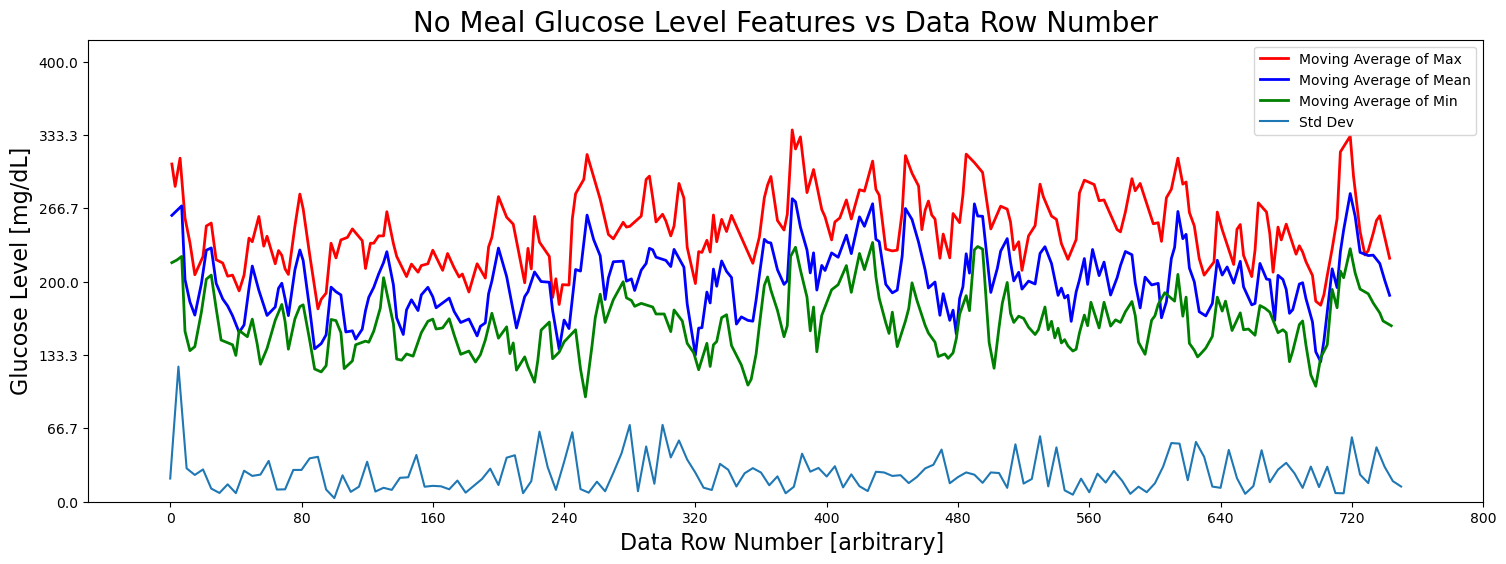
\includegraphics[width=0.7\linewidth]{files/adf7d67e6568598c773363d6a6979d27.png}

\subparagraph{Pairwise Plot of No Meal Features Matrix}

\begin{verbatim}
# Generate column labels for the features
feature_columns = [f'Feature_{i+1}' for i in range(meal_features_matrix.shape[1])]

# Convert the feature matrix to a Pandas DataFrame
df = pd.DataFrame(no_meal_features_matrix, columns=feature_columns)

# Create a pairwise plot using Seaborn
plt.figure(figsize=(15, 15))  # Adjust figure size as needed
sns.pairplot(df, diag_kind='hist', plot_kws={'alpha': 0.5, 's': 40})

plt.suptitle('Pairwise Plot of No Meal Features Matrix', y=1.02, fontsize=30)

# Show the plot
plt.show()
\end{verbatim}

\begin{verbatim}
<Figure size 1500x1500 with 0 Axes>
\end{verbatim}

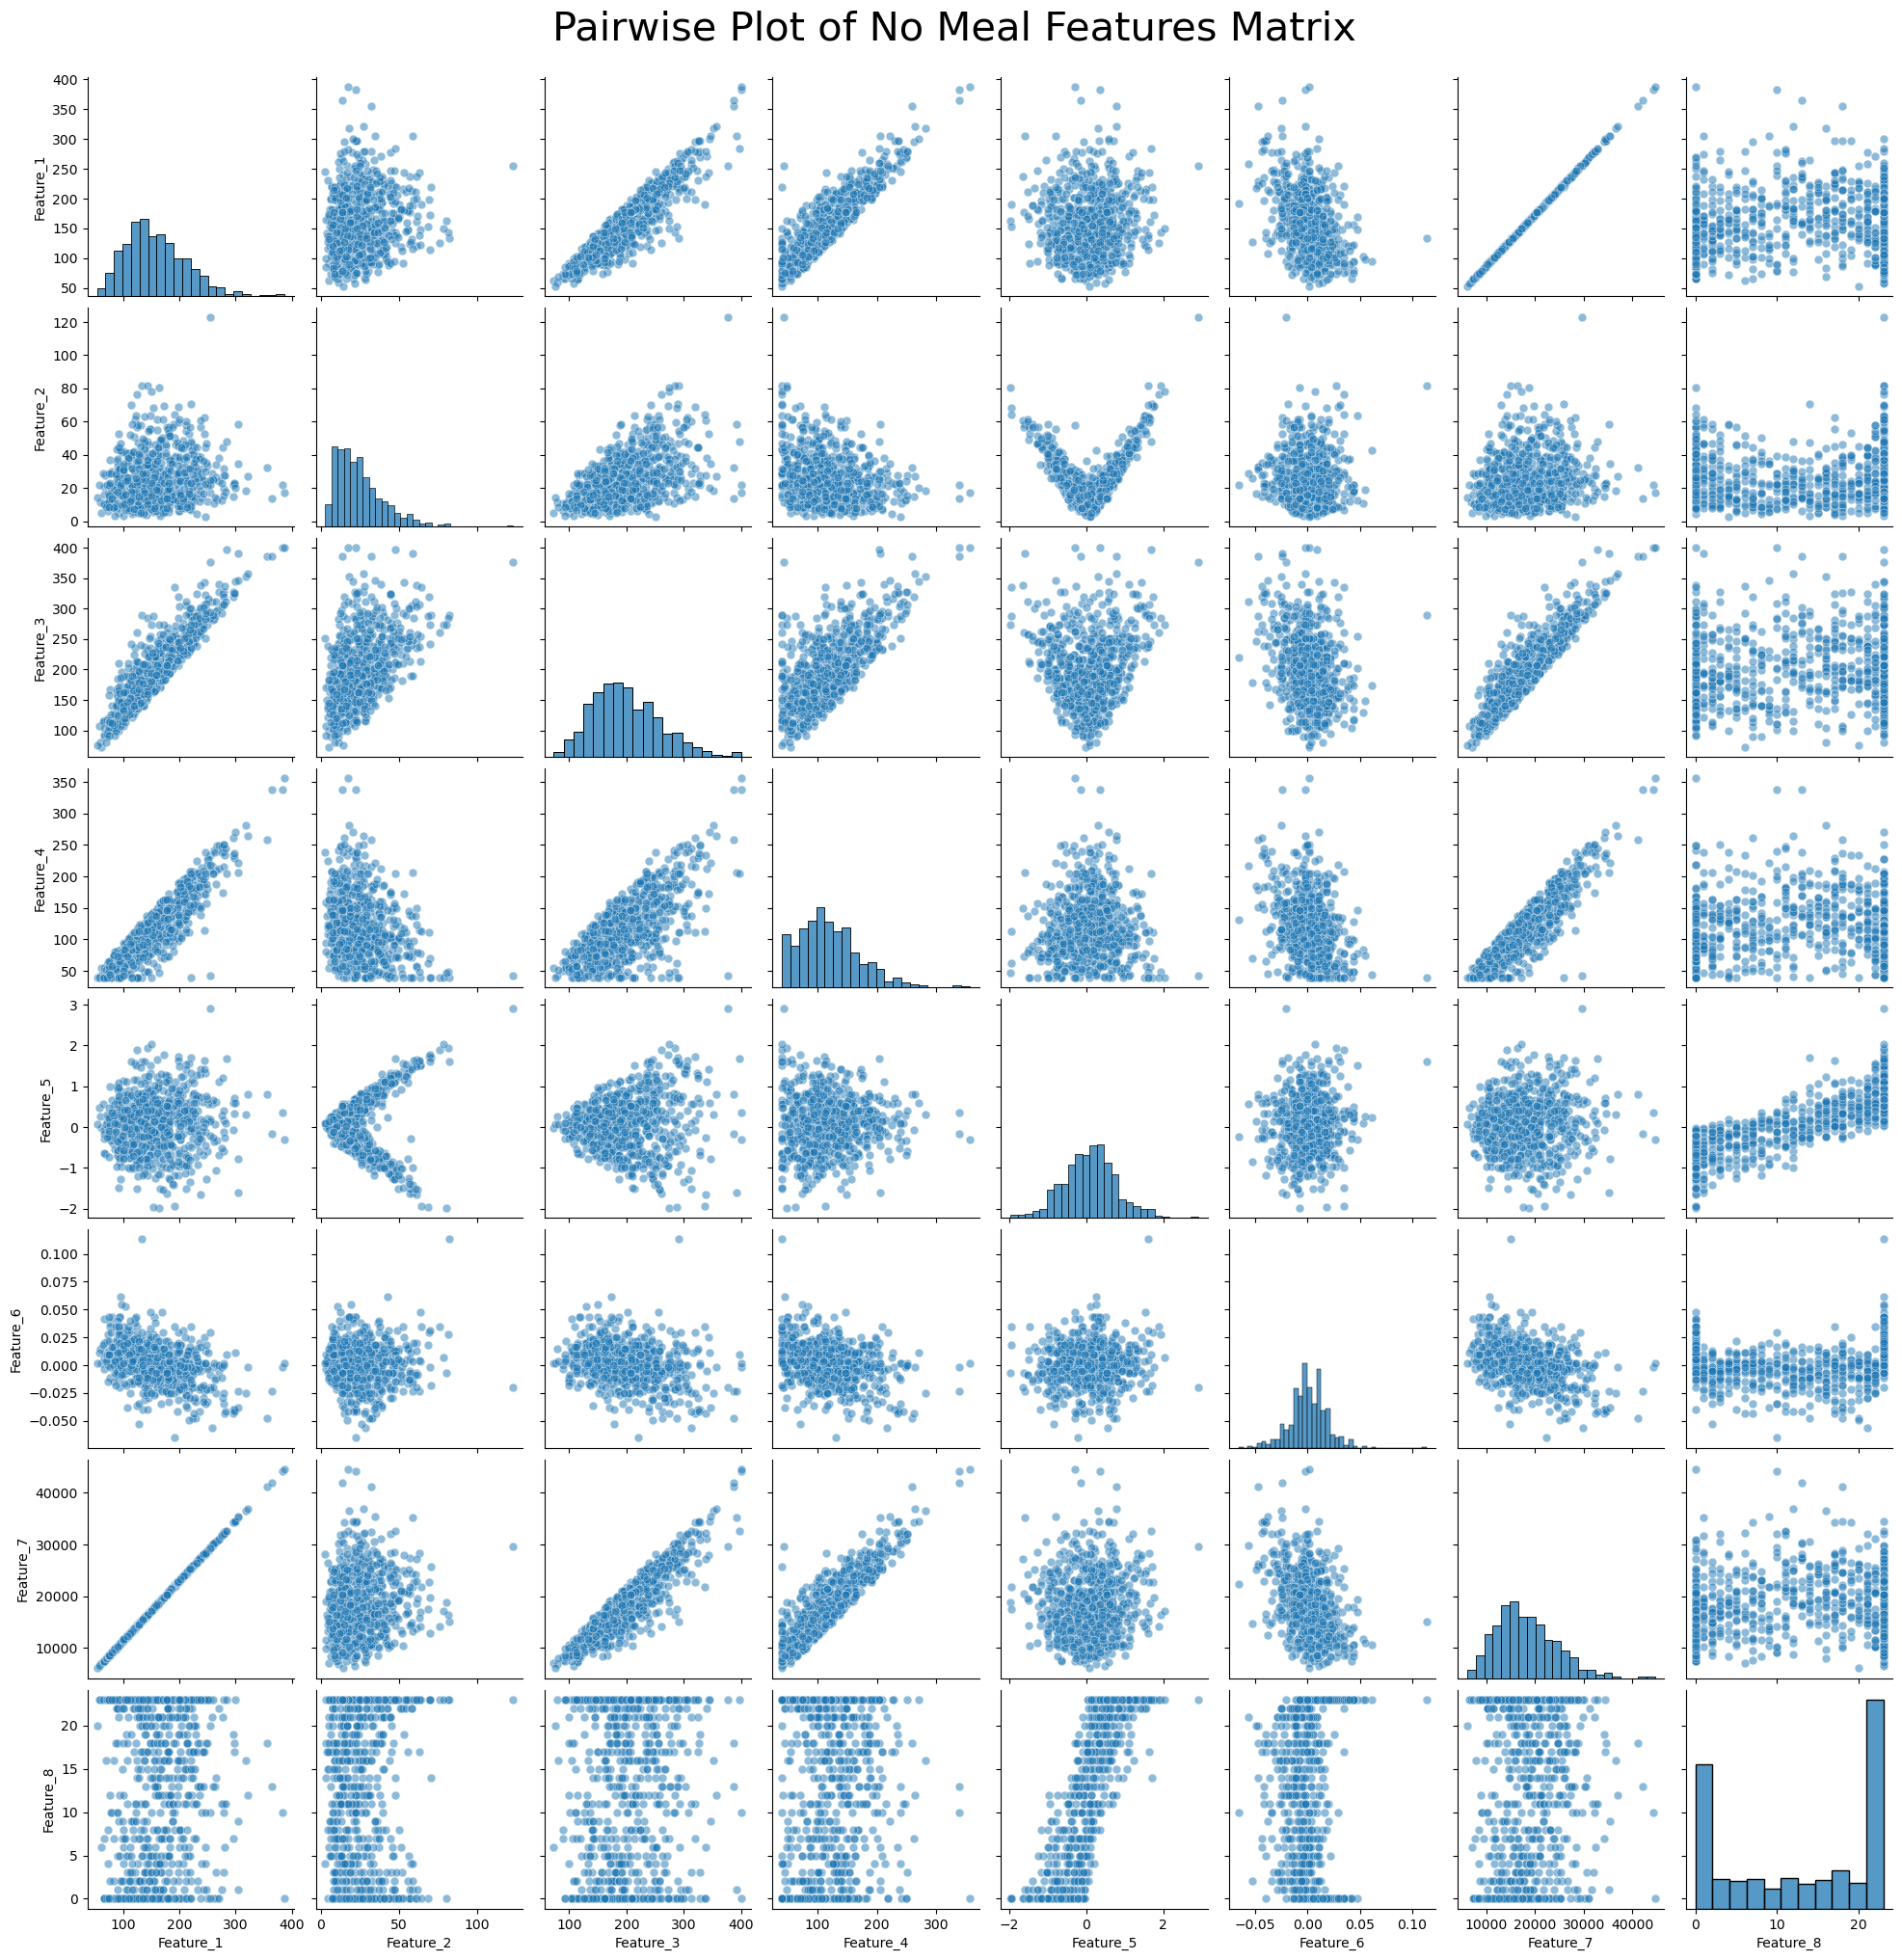
\includegraphics[width=0.7\linewidth]{files/fdede4157f769963ff3d36f16540e6ad.png}

\subparagraph{Concatenate Feature Matrices and Add Class Labels}

\begin{verbatim}
meal_labels = np.ones((meal_features_matrix.shape[0], 1))
len(meal_labels)
\end{verbatim}

\begin{verbatim}
944
\end{verbatim}

\begin{verbatim}
meal_features_matrix_with_labels = \
    np.hstack((meal_features_matrix, meal_labels))
#meal_features_matrix_with_labels[1]
\end{verbatim}

\begin{verbatim}
no_meal_labels = np.zeros((no_meal_features_matrix.shape[0], 1))
len(no_meal_labels)
\end{verbatim}

\begin{verbatim}
752
\end{verbatim}

\begin{verbatim}
no_meal_features_matrix_with_labels = \
    np.hstack((no_meal_features_matrix, no_meal_labels))
#no_meal_features_matrix_with_labels[1]
\end{verbatim}

\begin{verbatim}
concat_features = \
    np.vstack((meal_features_matrix_with_labels, no_meal_features_matrix_with_labels))
len(concat_features)
\end{verbatim}

\begin{verbatim}
1696
\end{verbatim}

\subparagraph{Train Support Vector Machine}

\subparagraph{Use Standard Variable Names for Features and Class Label}

\begin{verbatim}
X = concat_features[:, : -1]
y = concat_features[:, -1]
\end{verbatim}

\begin{verbatim}
X[0]
\end{verbatim}

\begin{verbatim}
array([ 8.98190476e+01,  1.91175360e+01,  1.31000000e+02,  4.90000000e+01,
       -2.82758621e -01, -4.28571429e -03,  1.30310714e+04,  9.00000000e+00])
\end{verbatim}

\begin{verbatim}
y[0]
\end{verbatim}

\begin{verbatim}
np.float64(1.0)
\end{verbatim}

\subparagraph{Train / Test Split}

\begin{verbatim}
X_train, X_test, y_train, y_test = \
    train_test_split(X, y, test_size = 0.2, random_state=40)
\end{verbatim}

\subparagraph{Normalize The Data}

\begin{verbatim}
scaler = StandardScaler()
X_train_scaled = scaler.fit_transform(X_train)
X_test_scaled = scaler.fit_transform(X_test)
\end{verbatim}

\subparagraph{Train SVM Model}

\begin{verbatim}
svm_model = SVC(kernel='linear', C=0.1)
svm_model.fit(X_train_scaled, y_train)
\end{verbatim}

\begin{verbatim}
SVC(C=0.1, kernel='linear')
\end{verbatim}

\textbf{In a Jupyter environment, please rerun this cell to show the HTML representation or trust the notebook. \newline
On GitHub, the HTML representation is unable to render, please try loading this page with nbviewer.org.}

[x]~~SVC\href{https://scikit-learn.org/1.5/modules/generated/sklearn.svm.SVC.html}{?Documentation for SVC}iFitted\begin{verbatim}
SVC(C=0.1, kernel='linear')
\end{verbatim}

\subparagraph{Test SVM Model}

\begin{verbatim}
y_pred = svm_model.predict(X_test_scaled)
\end{verbatim}

\subparagraph{Obtain Accuracy of SVM Model}

\begin{verbatim}
accuracy = accuracy_score(y_test, y_pred)
print(f"Accuracy: {accuracy * 100:.2f}%")
\end{verbatim}

\begin{verbatim}
Accuracy: 99.71%
\end{verbatim}

\subparagraph{Obtain Training and Test Accuracy of SVM Model}

\begin{verbatim}
train_accuracy = svm_model.score(X_train_scaled, y_train)
test_accuracy = svm_model.score(X_test_scaled, y_test)
print(f"Training Accuracy: {train_accuracy * 100:.2f}%")
print(f"Test Accuracy: {test_accuracy * 100:.2f}%")
\end{verbatim}

\begin{verbatim}
Training Accuracy: 100.00%
Test Accuracy: 99.71%
\end{verbatim}

\subparagraph{Obtain F1 Score of SVM Model}

\begin{verbatim}
f1 = f1_score(y_test, y_pred)
print(f"F1 Score: {f1:.2f}")
\end{verbatim}

\begin{verbatim}
F1 Score: 1.00
\end{verbatim}

\subparagraph{Cross Validate SVM Model}

\begin{verbatim}
scores = cross_val_score(svm_model, X_train_scaled, y_train, cv=5, scoring='accuracy')
print(f"Cross -Validation Accuracy: {scores.mean():.2f} (+/ - {scores.std():.2f})")
\end{verbatim}

\begin{verbatim}
Cross -Validation Accuracy: 1.00 (+/ - 0.00)
\end{verbatim}

\subparagraph{Visualize Results of SVM Model}

\subparagraph{Scatter Plot with PCA}

\begin{verbatim}
# Reduce dimensions using PCA
pca = PCA(n_components=2)

X_reduced = pca.fit_transform(X_test_scaled)

components = pca.components_
print(components)

# Get the predicted labels
predicted_labels = svm_model.predict(X_test_scaled)

# Create boolean masks for correct and incorrect predictions
correct_mask = (predicted_labels == y_test)
incorrect_mask = ~correct_mask

# Create a figure
plt.figure(figsize=(10, 6))

# Plot correct predictions in green
plt.scatter(X_reduced[correct_mask, 0], X_reduced[correct_mask, 1], color='green',
            marker='o', alpha=0.7, s=60, label='Correct Prediction')

# Plot incorrect predictions in red
plt.scatter(X_reduced[incorrect_mask, 0], X_reduced[incorrect_mask, 1], color='red',
            marker='x', alpha=0.7, s=60, label='Incorrect Prediction')

# Set labels and title
plt.xlabel('PCA Component 1', fontsize=20)
plt.ylabel('PCA Component 2', fontsize=20)
plt.title('SVM Classification Results: Correct vs Incorrect Predictions on Test Data', fontsize=18)

# Add a legend
plt.legend()

# Display the plot
plt.tight_layout()
plt.show()
\end{verbatim}

\begin{verbatim}
[[ 0.51111341  0.13118439  0.47327076  0.4251986   0.00643744 -0.257121
   0.50031459  0.01753109]
 [ -0.03692307  0.31993471  0.1095569  -0.19047139  0.66528982  0.06390289
   0.01416038  0.63332595]]
\end{verbatim}

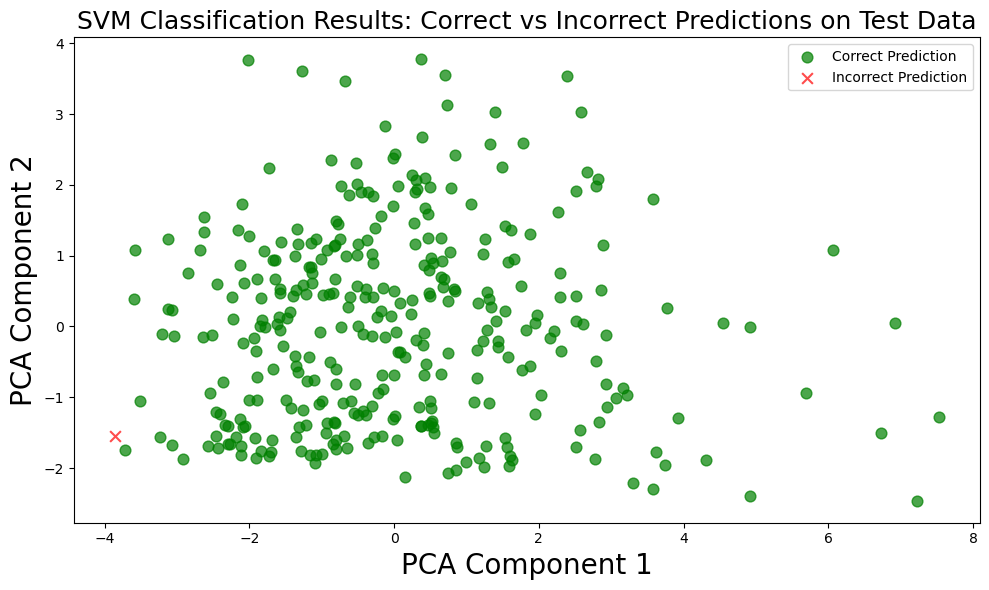
\includegraphics[width=0.7\linewidth]{files/5c63e3d289033a639c6b7a782c09b34c.png}

\subparagraph{Pairwise Plotting of Feature vs Feature}

\begin{verbatim}
df = pd.DataFrame(X_test_scaled, columns=[f'Feature {i+1}' for i in range(X_test_scaled.shape[1])])
df['Predicted Class'] = svm_model.predict(X_test_scaled)

# Plot pairwise relationships
sns.pairplot(df, hue='Predicted Class', palette='viridis')
plt.suptitle('Pair Plot of SVM Classification Results', y=1.02, fontsize=30)
plt.show()
\end{verbatim}

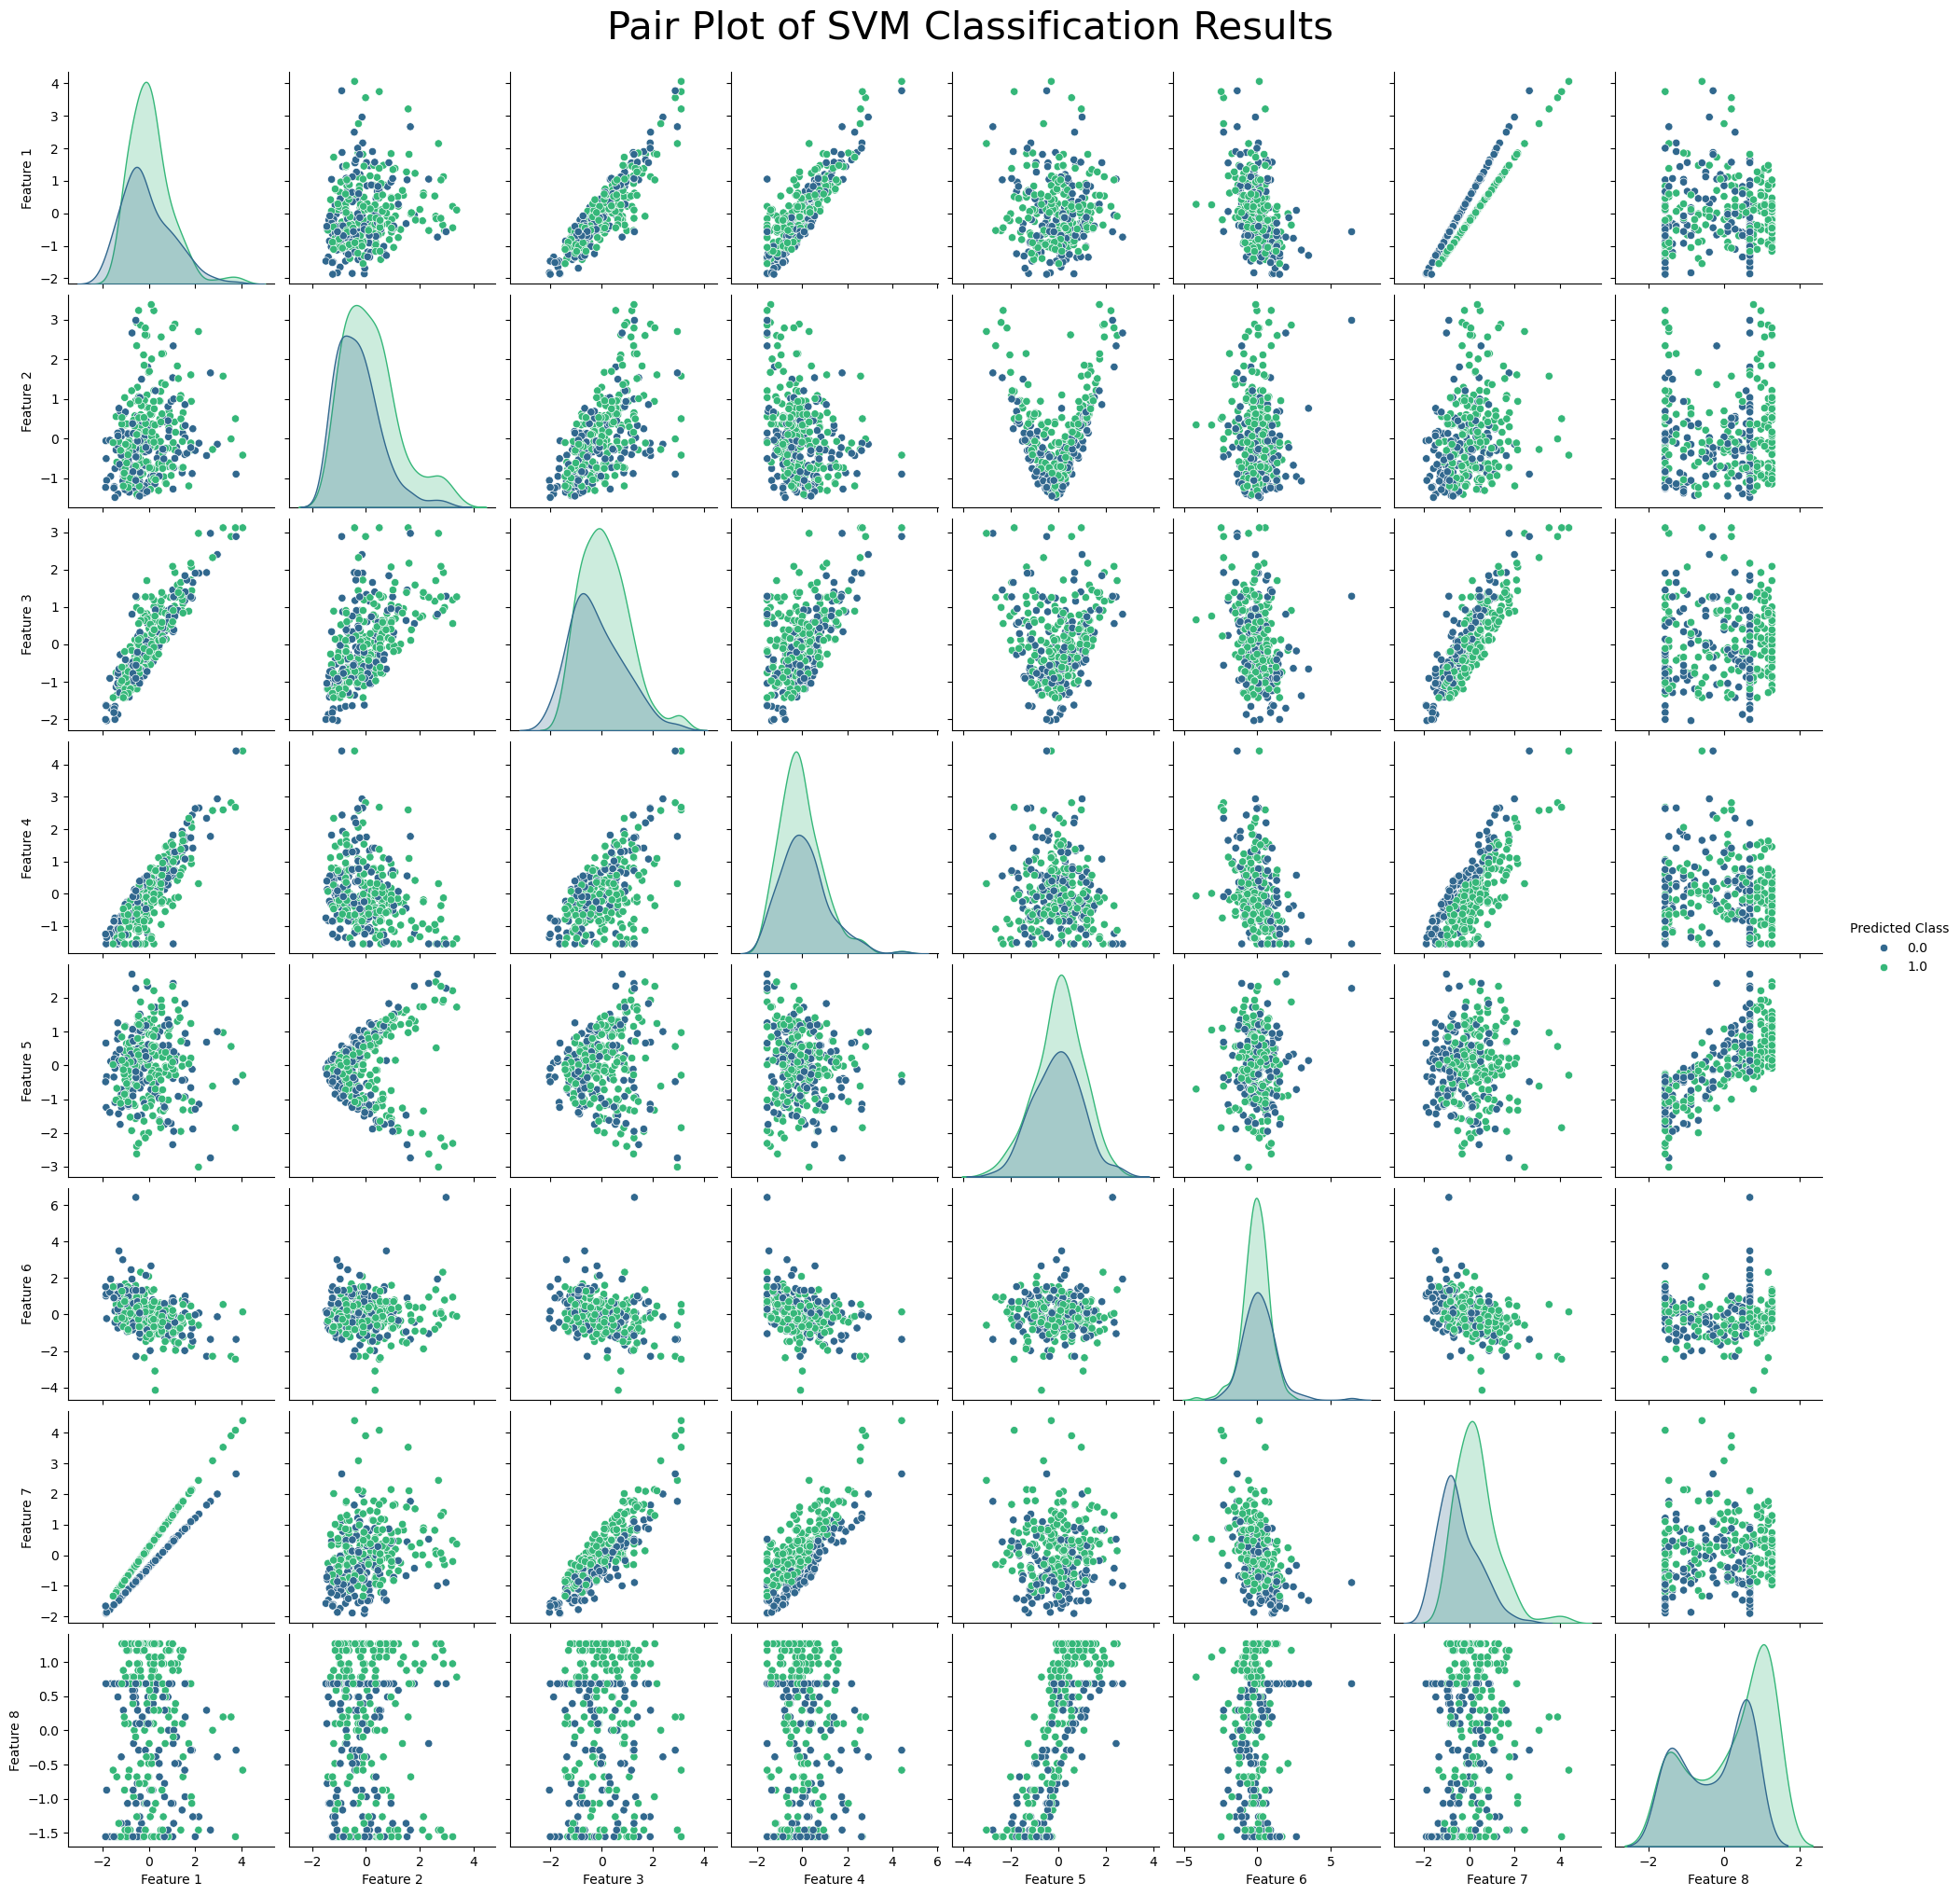
\includegraphics[width=0.7\linewidth]{files/8b4b5acb8b0d4a6b5b3f8937e7b09d1b.png}

\subparagraph{Heatmaps of Confusion Matrix}

\begin{verbatim}
# Get the predicted classes
y_pred = svm_model.predict(X_test_scaled)

# Create the confusion matrix
cm = confusion_matrix(y_test, y_pred)

# Plot the heatmap of the confusion matrix
sns.heatmap(cm, annot=True, cmap='Blues', fmt='d')
plt.xlabel('Predicted')
plt.ylabel('Actual')
plt.title('Confusion Matrix Heatmap of Test Data')
plt.show()


# Print accuracy, recall, precision, and F1 score
accuracy = accuracy_score(y_test, y_pred)
recall = recall_score(y_test, y_pred)
precision = precision_score(y_test, y_pred)
f1 = f1_score(y_test, y_pred)

print(f'Accuracy: {accuracy:.4f}')
print(f'Recall: {recall:.4f}')
print(f'Precision: {precision:.4f}')
print(f'F1 Score: {f1:.4f}')
\end{verbatim}

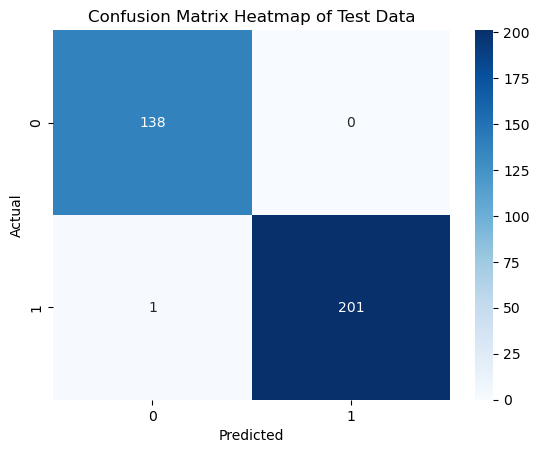
\includegraphics[width=0.7\linewidth]{files/316fae2de0eebc02e06b1573c013a345.png}

\begin{verbatim}
Accuracy: 0.9971
Recall: 0.9950
Precision: 1.0000
F1 Score: 0.9975
\end{verbatim}

\subparagraph{Dump Model to Pickle File}

\begin{verbatim}
with open('svm_model.pkl', 'wb') as f:
    pickle.dump(svm_model, f)
\end{verbatim}